\documentclass{ucbthesis}

\usepackage[usenames, dvipsnames]{color}
\usepackage{hyperref}
\hypersetup{
  colorlinks=true,
  urlcolor=MidnightBlue,
  linkcolor=MidnightBlue,
  citecolor=ForestGreen,
  pdfinfo={
    CreationDate={D:20180629134841},
    ModDate={D:20180629134841},
  },
}

%% % Double spacing, if you want it.
%% \def\dsp{\def\baselinestretch{2.0}\large\normalsize}
%% \dsp

% If the Grad. Division insists that the first paragraph of a section
% be indented (like the others), then include this line:
\usepackage{indentfirst}

\usepackage{amsthm,amssymb,amsmath}
\allowdisplaybreaks
\usepackage{textcomp}
%% H/T: https://tex.stackexchange.com/a/56877/32270
\usepackage{algorithm}
\usepackage{algpseudocode}
%% H/T: https://tex.stackexchange.com/a/244805
\usepackage{booktabs,siunitx}
%% H/T: https://tex.stackexchange.com/a/4217/32270
\usepackage{mathtools}
%% H/T: https://tex.stackexchange.com/a/33869/32270
\makeatletter
\newenvironment{breakablealgorithm}
  {% \begin{breakablealgorithm}
   \begin{center}
     \refstepcounter{algorithm}% New algorithm
     \hrule height.8pt depth0pt \kern2pt% \@fs@pre for \@fs@ruled
     \renewcommand{\caption}[2][\relax]{% Make a new \caption
       {\raggedright\textbf{\ALG@name~\thealgorithm} ##2\par}%
       \ifx\relax##1\relax % #1 is \relax
         \addcontentsline{loa}{algorithm}{\protect\numberline{\thealgorithm}##2}%
       \else % #1 is not \relax
         \addcontentsline{loa}{algorithm}{\protect\numberline{\thealgorithm}##1}%
       \fi
       \kern2pt\hrule\kern2pt
     }
  }{% \end{breakablealgorithm}
     \kern2pt\hrule\relax% \@fs@post for \@fs@ruled
   \end{center}
  }
\makeatother
%% H/T: https://tex.stackexchange.com/a/28334/32270
\usepackage{chngcntr}
\counterwithin{figure}{chapter}
\counterwithin{table}{chapter}
\counterwithin{equation}{chapter}
\counterwithin{algorithm}{chapter}
%% H/T: https://tex.stackexchange.com/a/202047/32270
%%      https://tex.stackexchange.com/a/32463/32270
\usepackage[labelfont=bf]{caption}
%% H/T: https://tex.stackexchange.com/a/163250/32270
\usepackage{adjustbox}

\theoremstyle{definition}
\newtheorem{theorem}{Theorem}[section]
\newtheorem{lemma}{Lemma}[section]
\counterwithin{theorem}{chapter}
\counterwithin{lemma}{chapter}

\renewcommand{\qed}{\(\blacksquare\)}
\newcommand{\eps}{\varepsilon}
\newcommand{\cond}[1]{\operatorname{cond}\left(#1\right)}
\newcommand{\fl}[1]{\operatorname{fl}\left(#1\right)}
\newcommand{\bigO}[1]{\mathcal{O}\left(#1\right)}
\newcommand{\mach}{\mathbf{u}}
\newcommand{\utri}{\mathcal{U}}
%% db == ``delta'' b
\newcommand{\db}[1]{
  \ifthenelse{\equal{#1}{1}}
             {\partial b}
             {\partial^{#1} b}
}
%% cdb == computed ``delta'' b
\newcommand{\cdb}[1]{
  \ifthenelse{\equal{#1}{1}}
             {\widehat{\partial b}}
             {\widehat{\partial^{#1} b}}
}

\hyphenation{mar-gin-al-ia}
%% H/T: https://latex.org/forum/viewtopic.php?t=2351
\setcounter{secnumdepth}{3}
\setcounter{tocdepth}{3}
%% H/T: https://tex.stackexchange.com/a/26348/32270
\renewcommand*{\appendixname}{}

\begin{document}

% Declarations for Front Matter

\title{High-order Lagrangian Methods and Computations on Curved Elements}
\author{Danny Hermes}
\degreesemester{Summer}
\degreeyear{2018}
\degree{Doctor of Philosophy}
\chair{Professor Per-Olof Persson}
\othermembers{Professor John Strain \\ Professor TODO}
\numberofmembers{3}
\prevdegrees{B.S. (University of Michigan) 2010}
\field{Applied Mathematics}
\campus{Berkeley}

\maketitle
\approvalpage
\copyrightpage

\begin{abstract}
In computer aided geometric design a polynomial is usually represented in
Bernstein form. This paper presents a family of compensated algorithms to
accurately evaluate a polynomial in Bernstein form with floating point
coefficients. The principle is to apply error-free transformations to
improve the traditional de Casteljau algorithm. At each stage of computation,
round-off error is passed on to first order errors, then to second order
errors, and so on. After the computation has been ``filtered'' \((K - 1)\)
times via this process, the resulting output is as accurate as the de Casteljau
algorithm performed in \(K\) times the working precision. Forward error
analysis and numerical experiments illustrate the accuracy of this family
of algorithms.
\end{abstract}


\begin{frontmatter}

\begin{dedication}
\null\vfil
\begin{center}
To my wife Sharona and my sons Jack and Max.
\end{center}
\vfil\null
\end{dedication}

\tableofcontents
\clearpage
\listoffigures
\clearpage
\listoftables

\begin{acknowledgements}
I want to thank my advisor for his patience and guidance.
\end{acknowledgements}

\end{frontmatter}

\pagestyle{headings}

\chapter{Introduction}

This is a work in two parts, each in a different subfield of mathematics.
The first part is a general-purpose tool for computational physics problems.
The tool enables data transfer across two curved meshes.
Since the tool requires a significant amount of computational geometry, the
second half focuses on computational geometry. In particular, it considers
cases where the geometric methods used have seriously degraded accuracy due to
ill-conditioning.

\section{Computational Physics}

In computational physics, the problem of data transfer between meshes
occurs in several applications. For example, by allowing the underyling
computational domain to change during a simulation, computational
effort can be focused dynamically to resolve sensitive features
of a numerical solution. Mesh adaptivity (see, for example,
\cite{Dukowicz1987, Babuska1978}), this in-flight change in the mesh,
requires translating the numerical solution from the old mesh to the new,
i.e. data transfer. As another example, Lagrangian or particle-based methods
treat each node in mesh as a particle and so with each timestep the mesh
travels \textbf{with} the fluid (see, for example, \cite{Hirt1974}).
However, over (typically limited) time the mesh
becomes distorted and suffers a loss in element quality which causes
catastrophic loss in the accuracy of computation. To overcome this, the
domain must be remeshed or rezoned and the solution must be
transferred (remapped) onto the new mesh configuration.

When pointwise interpolation is used to transfer a solution, quantities with
physical meaning (e.g. mass, concentration, energy) may not be conserved.
To address this, there have been many explorations (for example,
\cite{Jiao2004, Farrell2009, Farrell2011}) of
\textbf{conservative interpolation} (typically using Galerkin or
\(L_2\)-minimizing methods). In this work, the author introduces a
conservative interpolation method for data transfer between high-order
meshes. These high-order meshes are typically curved, but not necessarily
all elements or at all timesteps.

The existing work on data transfer has considered straight-sided meshes,
which use shape functions that have degree \(p = 1\) to represent solutions
on each element. However, both to allow for greater geometric flexibility
and for high-order of convergence, this work will consider the case
of curved isoparametric\footnote{I.e. the degree of the discrete field on the
mesh is same as the degree of the shape functions that determine the
mesh.} meshes. Allowing curved geometries is useful since many practical
problems involve geometries that change over time, such as flapping flight
or fluid-structure interactions. In addition, high-order CFD methods
(\cite{Wang2013}) have the ability to produce highly accurate solutions
with low dissipation and low dispersion error.

\section{Computational Geometry}

For a function in Bernstein form, the condition number of evaluation
becomes infinite as the input approaches a root. Similarly,
as a (transversal) intersection of two B\'{e}zier curves approaches a
point of tangency, the condition number of intersection becomes
infinite. These breakdowns in accuracy cause problems when evaluating
integrals on elements of a curved mesh or on the intersections of two
elements. For example, consider the problem of data transfer from
one mesh to another. As both meshes are refined simultaneously, the
probability of an ``almost tangent'' pair of curved edges increases
towards unity. Tangent curves correspond to the case of a double root
of a polynomial. Though they are unlikely for a random mesh pair
``double roots, though rare, are overwhelmingly more common in practice
than are roots of higher multiplicity'' (\cite{Kahan1972}, page 6).

Two approaches will be described that can help recover this lost accuracy
in the presence of ill-conditioning. The first allows for greater
accuracy when performing the de Casteljau algorithm to evaluate
a function in Bernstein form. This \textbf{compensated algorithm}
(Chapter~\ref{chap:k-compensated}) produces results that are as accurate as if
the computations were done in \(K\) times the working precision
and then rounded back to the working precision. By just using a
more precise evaluation of the residual function,
\cite{Tisseur2001} showed that the accuracy of Newton's method can
be improved. So as a natural extension, the second approach
explores the improvement in Newton's method applied both to
root-finding and B\'{e}zier curve intersection
(Chapter~\ref{chap:compensated-newton}).

\section{Organization}

This work is organized as follows. Chapter~\ref{chap:preliminaries}
establishes common notation and reviews basic results relevant to the
topics at hand. Chapter~\ref{chap:bezier-intersection} is an
in-depth discussion of the computational geometry methods needed
to implement to enable data transfer. Chapter~\ref{chap:data-transfer}
describes the data transfer process and gives results of some
numerical experiments confirming the rate of convergence.
Chapter~\ref{chap:k-compensated} describes a compensated algorithm for
evaluating functions in Bernstein form (such as B\'{e}zier curves);
this algorithm produces results that are as accurate as if
the computations were done in \(K\) times the working precision
and then rounded back to the working precision.
Chapter~\ref{chap:compensated-newton} describes two modified Newton's
methods which allow for greater accuracy in the presence of
ill-conditioning; one is used for computing simple zeros
of polynomials in Bernstein form and the other for computing
B\'{e}zier curve intersections.

\chapter{Preliminaries}\label{chap:preliminaries}

\section{General Notation}

We'll refer to \(\reals\) for the reals, \(\utri\) represents
the unit triangle (or unit simplex) in \(\reals^2\):
\(\utri = \left\{(s, t) \mid 0 \leq s, t, s + t \leq 1\right\}\).
When dealing with sequences with multiple indices, e.g.
\(s_{m, n} = m + n\), we'll use bold symbols to represent
a multi-index: \(\bm{i} = (m, n)\). We'll use \(\left|\bm{i}\right|\) to
represent the sum of the components in a multi-index.
The binomial coefficient
\(\binom{n}{k}\) is equal to \(\frac{n!}{k! (n - k)!}\) and the trinomial
coefficient \(\binom{n}{i, j, k}\) is equal to \(\frac{n!}{i! j! k!}\)
(where \(i + j + k = n\)). The notation \(\delta_{ij}\) represents the
Kronecker delta, a value which is \(1\) when \(i = j\) and \(0\)
otherwise.

\section{Floating Point and Forward Error Analysis}

We assume all floating point operations obey
\begin{equation}
  a \star b = \fl{a \circ b} = (a \circ b)(1 + \delta_1) =
  (a \circ b) / (1 + \delta_2)
\end{equation}
where \(\star \in \left\{\oplus, \ominus, \otimes, \oslash\right\}\), \(\circ
\in \left\{+, -, \times, \div\right\}\) and \(\left|\delta_1\right|,
\left|\delta_2\right| \leq \mach\). The symbol \(\mach\) is the unit round-off
and \(\star\) is a floating point operation, e.g.
\(a \oplus b = \fl{a + b}\). (For IEEE-754 floating point double precision,
\(\mach = 2^{-53}\).) We denote the computed result of
\(\alpha \in \reals\) in floating point arithmetic by
\(\widehat{\alpha}\) or \(\fl{\alpha}\) and use \(\floats\) as the set of
all floating point numbers (see \cite{Higham2002} for more details).
Following \cite{Higham2002}, we will use the following classic properties in
error analysis.

\begin{enumerate}
  \item If \(\delta_i \leq \mach\), \(\rho_i = \pm 1\), then
      \(\prod_{i = 1}^n (1 + \delta_i)^{\rho_i} = 1 + \theta_n\),
  \item \(\left|\theta_n\right| \leq \gamma_n \coloneqq
      n \mach / (1 - n \mach)\),
  \item \((1 + \theta_k)(1 + \theta_j) = 1 + \theta_{k + j}\),
  \item \(\gamma_k + \gamma_j + \gamma_k \gamma_j \leq \gamma_{k + j}
    \Longleftrightarrow (1 + \gamma_k)(1 + \gamma_j) \leq 1 + \gamma_{k + j}\),
  \item \((1 + \mach)^j \leq 1 / (1 - j \mach) \Longleftrightarrow
  (1 + \mach)^j - 1 \leq \gamma_j\).
\end{enumerate}

\section{B\'{e}zier Curves}

A \textbf{B\'{e}zier curve} is a mapping from the unit interval
that is determined by a set of control points
\(\left\{\bm{p}_j\right\}_{j = 0}^n \subset \reals^d\).
For a parameter \(s \in \left[0, 1\right]\), there is a corresponding
point on the curve:
\begin{equation}
b(s) = \sum_{j = 0}^n \binom{n}{j} (1 - s)^{n - j} s^j \bm{p}_j \in
  \reals^d.
\end{equation}
This is a combination of the control points weighted by
each Bernstein basis function
\(B_{j, n}(s) = \binom{n}{j} (1 - s)^{n - j} s^j\).
Due to the binomial expansion
\(1 = (s + (1 - s))^n = \sum_{j = 0}^n B_{j, n}(s)\),
a Bernstein basis function is in
\(\left[0, 1\right]\) when \(s\) is as well. Due to this fact, the
curve must be contained in the convex hull of it's control points.

\subsection{de Casteljau Algorithm}

Next, we recall\footnote{We have used slightly non-standard notation for the
terms produced by the de Casteljau algorithm: we start the superscript at
\(n\) and count down to \(0\) as is typically done when describing Horner's
algorithm. For example, we use \(b_j^{(n - 2)}\) instead of
\(b_j^{(2)}\).} the de Casteljau algorithm:

\begin{breakablealgorithm}
  \caption{\textit{de Casteljau algorithm for polynomial evaluation.}}
  \label{alg:de-casteljau}

  \begin{algorithmic}
    \Function{\(\mathtt{result} = \mathtt{DeCasteljau}\)}{$b, s$}
      \State \(n = \texttt{length}(b) - 1\)
      \State \(\widehat{r} = 1 \ominus s\)
      \\
      \For{\(j = 0, \ldots, n\)}
        \State \(\widehat{b}_j^{(n)} = b_j\)
      \EndFor
      \\
      \For{\(k = n - 1, \ldots, 0\)}
        \For{\(j = 0, \ldots, k\)}
          \State \(\widehat{b}_j^{(k)} = \left(
              \widehat{r} \otimes \widehat{b}_j^{(k + 1)}\right) \oplus
              \left(s \otimes \widehat{b}_{j + 1}^{(k + 1)}\right)\)
        \EndFor
      \EndFor
      \\
      \State \(\mathtt{result} = \widehat{b}_0^{(0)}\)
    \EndFunction
  \end{algorithmic}
\end{breakablealgorithm}

\begin{theorem}[\cite{Mainar1999}, Corollary 3.2]
If \(p(s) = \sum_{j = 0}^n b_j B_{j, n}(s)\) and \(\mathtt{DeCasteljau}(p, s)\)
is the value computed by the de Casteljau algorithm then\footnote{In the
original paper the factor on \(\widetilde{p}(s)\) is \(\gamma_{2n}\),
but the authors did not consider round-off when computing
\(1 \ominus s\).}
\begin{equation}
\left|p(s) - \mathtt{DeCasteljau}(p, s)\right| \leq \gamma_{3n}
\sum_{j = 0}^n \left|b_j\right| B_{j, n}(s).
\end{equation}
\end{theorem}

The relative condition number of the evaluation of \(p(s) = \sum_{j = 0}^n
b_j B_{j, n}(s)\) in Bernstein form used in this work is (see
\cite{Mainar1999, Farouki1987}):
\begin{equation}
\cond{p, s} = \frac{\widetilde{p}(s)}{\left|p(s)\right|},
\end{equation}
where
\(\widetilde{p}(s) \coloneqq \sum_{j = 0}^n \left|b_j\right| B_{j, n}(s)\).

To be able to express the algorithm in matrix form, we define
the vectors
\begin{equation}
b^{(k)} = \left[\begin{array}{c c c} b_0^{(k)} & \cdots &
b_k^{(k)}\end{array}\right]^T, \quad
\widehat{b}^{(k)} = \left[\begin{array}{c c c} \widehat{b}_0^{(k)} & \cdots &
    \widehat{b}_k^{(k)}\end{array}\right]^T
\end{equation}
and the reduction matrices:
\begin{equation}
U_k = U_k(s) = \left[\begin{array}{c c c c c c}
    1 - s  & s      & 0      & \cdots & \cdots & 0      \\
    0      & 1 - s  & s      & \ddots &        & \vdots \\
    \vdots & \ddots & \ddots & \ddots & \ddots & \vdots \\
    \vdots &        & \ddots & \ddots & \ddots & 0 \\
    0      & \cdots & \cdots & 0      & 1 - s  & s
\end{array}\right] \in \reals^{k \times (k + 1)}.
\end{equation}
With this, we can express (\cite{Mainar1999}) the de Casteljau algorithm as
\begin{equation}\label{eq:matrix-de-casteljau}
b^{(k)} = U_{k + 1} b^{(k + 1)}
\Longrightarrow b^{(0)} = U_1 \cdots U_n b^{(n)}.
\end{equation}

In general, for a sequence \(v_0, \ldots, v_n\) we'll refer to \(v\)
as the vector containing all of the values:
\(v = \left[\begin{array}{c c c} v_0 & \cdots &
    v_n\end{array}\right]^T.\)

\section{B\'{e}zier Triangles}

A \textbf{B\'{e}zier triangle} (\cite[Chapter~17]{Farin2001}) is a
mapping from the unit triangle
\(\utri\) and is determined by a control net
\(\left\{\bm{p}_{i, j, k}\right\}_{i + j + k = n} \subset \reals^d\).
A B\'{e}zier triangle is a particular kind of B\'{e}zier surface, i.e. one
in which there are two cartesian or three barycentric input parameters.
Often the term B\'{e}zier surface is used to refer to a tensor product or
rectangular patch.
For \((s, t) \in \utri\) we can define barycentric weights
\(\lambda_1 = 1 - s - t, \lambda_2 = s, \lambda_3 = t\) so that
\begin{equation}
1 = \left(\lambda_1 + \lambda_2 + \lambda_3\right)^n =
  \sum_{\substack{i + j + k = n \\ i, j, k \geq 0}} \binom{n}{i, j, k}
  \lambda_1^i \lambda_2^j \lambda_3^k.
\end{equation}
Using this we can similarly define a (triangular) Bernstein basis
\begin{equation}
B_{i, j, k}(s, t) = \binom{n}{i, j, k} (1 - s - t)^i s^j t^k
  = \binom{n}{i, j, k} \lambda_1^i \lambda_2^j \lambda_3^k
\end{equation}
that is in \(\left[0, 1\right]\) when \((s, t)\) is in \(\utri\).
Using this, we define points on the B\'{e}zier triangle as a
convex combination of the control net:
\begin{equation}
b(s, t) = \sum_{i + j + k = n} \binom{n}{i, j, k}
  \lambda_1^i \lambda_2^j \lambda_3^k
  \bm{p}_{i, j, k} \in \reals^d.
\end{equation}

\begin{figure}
  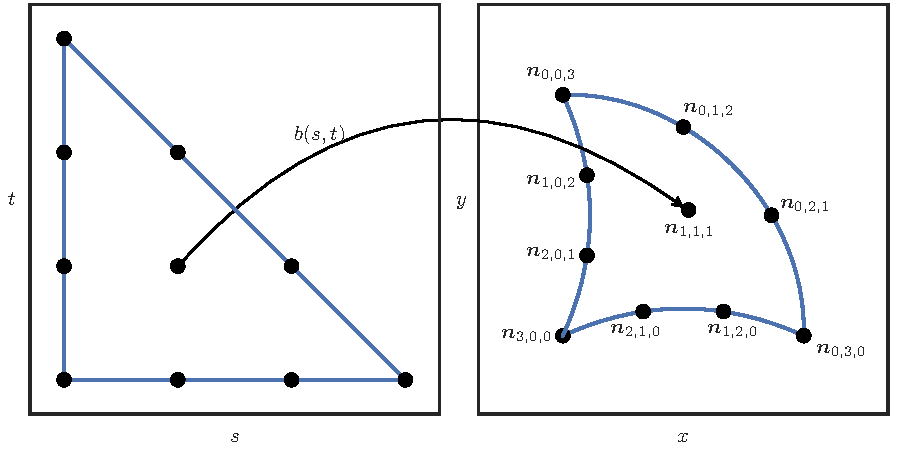
\includegraphics{../images/curved-mesh/main_figure01.pdf}
  \centering
  \captionsetup{width=.75\linewidth}
  \caption{Cubic B\'{e}zier triangle}
  \label{fig:cubic-bezier-example}
\end{figure}

\noindent Rather than defining a B\'{e}zier triangle by the control net, it can
also be uniquely determined by the image of a standard lattice of
points in \(\utri\): \(b\left(j/n, k/n\right) = \bm{n}_{i, j, k}\);
we'll refer to these as \textbf{standard nodes}.
Figure~\ref{fig:cubic-bezier-example} shows these standard nodes for
a cubic triangle in \(\reals^2\). To see the correspondence,
when \(p = 1\) the standard nodes \textbf{are} the control net
\begin{equation}
b(s, t) = \lambda_1 \bm{n}_{1, 0, 0} +
\lambda_2 \bm{n}_{0, 1, 0} + \lambda_3 \bm{n}_{0, 0, 1}
\end{equation}
and when \(p = 2\)
\begin{multline}
b(s, t) = \lambda_1\left(2 \lambda_1 - 1\right) \bm{n}_{2, 0, 0} +
\lambda_2\left(2 \lambda_2 - 1\right) \bm{n}_{0, 2, 0} +
\lambda_3\left(2 \lambda_3 - 1\right) \bm{n}_{0, 0, 2} + \\
4 \lambda_1 \lambda_2 \bm{n}_{1, 1, 0} +
4 \lambda_2 \lambda_3 \bm{n}_{0, 1, 1} +
4 \lambda_3 \lambda_1 \bm{n}_{1, 0, 1}.
\end{multline}
However, it's worth noting that the transformation between
the control net and the standard nodes has condition
number that grows exponentially with \(n\) (see~\cite{Farouki1991}, which
is related but does not directly show this).
This may make working with
higher degree triangles prohibitively unstable.

A \textbf{valid} B\'{e}zier triangle is one which is
diffeomorphic to \(\utri\), i.e. \(b(s, t)\) is bijective and has
an everywhere invertible Jacobian. We must also have the orientation
preserved, i.e. the Jacobian must have positive determinant. For example, in
Figure~\ref{fig:inverted-element}, the image of \(\utri\) under
the map \(b(s, t) = \left[\begin{array}{c c} (1 - s - t)^2 + s^2 & s^2 + t^2
\end{array}\right]^T\) is not valid because the Jacobian is zero along
the curve \(s^2 - st - t^2 - s + t = 0\) (the dashed line). Elements that
are not valid are called \textbf{inverted} because they have regions with
``negative area''. For the example, the image \(b\left(\utri\right)\)
leaves the boundary determined by the edge curves: \(b(r, 0)\),
\(b(1 - r, r)\) and \(b(0, 1 - r)\) when \(r \in \left[0, 1\right]\).
This region outside the boundary is traced twice, once with
a positive Jacobian and once with a negative Jacobian.
\begin{figure}
  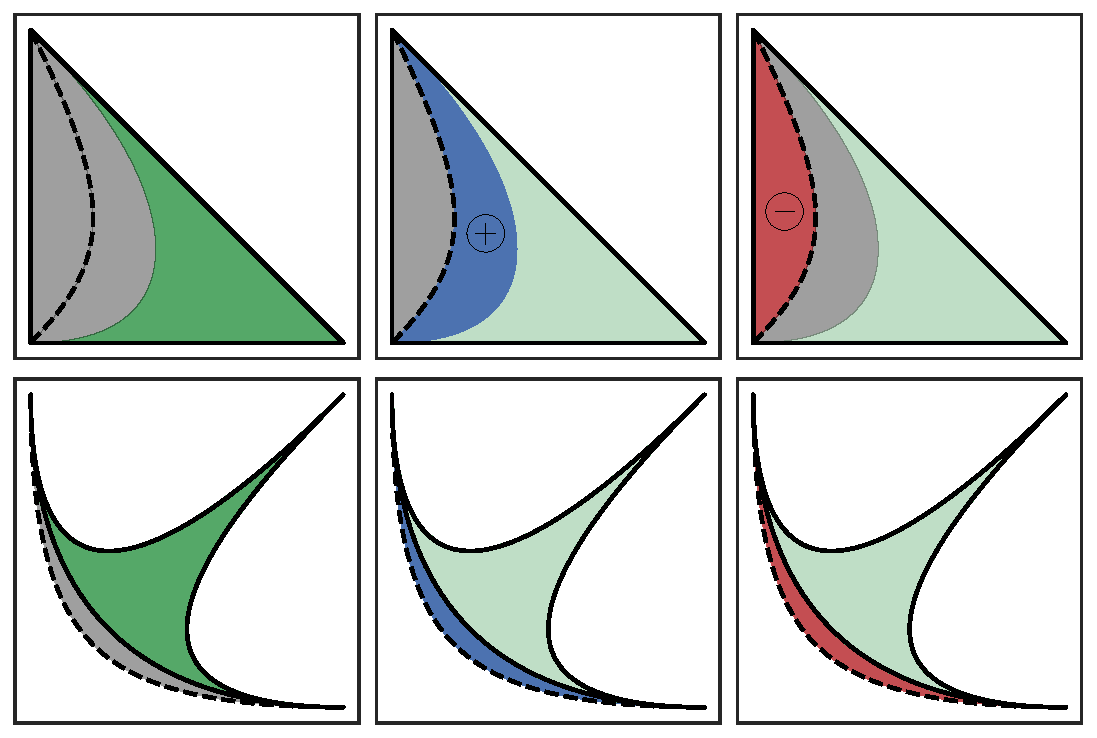
\includegraphics{../images/curved-mesh/inverted_element.pdf}
  \centering
  \captionsetup{width=.75\linewidth}
  \caption{The B\'{e}zier triangle given by \(b(s, t) = \left[
    (1 - s - t)^2 + s^2 \; \; s^2 + t^2 \right]^T\) produces an
    inverted element. It traces the same region twice, once with
    a positive Jacobian (the middle column) and once with a negative
    Jacobian (the right column).}
  \label{fig:inverted-element}
\end{figure}

\section{Curved Elements}\label{sec:curved-elements}

We define a curved mesh element \(\mathcal{T}\) of degree \(p\)
to be a B\'{e}zier triangle in \(\reals^2\) of the same degree.
We refer to the component functions of \(b(s, t)\) (the map that
gives \(\mathcal{T} = b\left(\utri\right)\)) as \(x(s, t)\) and \(y(s, t)\).

This fits a typical definition (\cite[Chapter~12]{FEM-ClaesJohnson})
of a curved element, but gives a special meaning to the mapping from
the reference triangle. Interpreting elements as B\'{e}zier triangles
has been used for Lagrangian methods where
mesh adaptivity is needed (e.g. ~\cite{CardozeMOP04}). Typically curved
elements only have one curved side (\cite{McLeod1972}) since they are used
to resolve geometric features of a boundary. See also
\cite{Zlmal1973, Zlmal1974}.
B\'{e}zier curves and triangles have a number of mathematical properties
(e.g. the convex hull property) that lead to elegant geometric
descriptions and algorithms.

Note that a B\'{e}zier triangle can be
determined from many different sources of data (for example the control net
or the standard nodes). The choice of this data may be changed to suit the
underlying physical problem without changing the actual mapping. Conversely,
the data can be fixed (e.g. as the control net) to avoid costly basis
conversion; once fixed, the equations of motion and other PDE terms can
be recast relative to the new basis (for an example, see \cite{Persson2009},
where the domain varies with time but the problem is reduced to
solving a transformed conservation law in a fixed reference configuration).

\subsection{Shape Functions}\label{subsec:shape-functions}

When defining shape functions (i.e. a basis with geometric meaning) on a
curved element there are (at least) two choices. When the degree of the
shape functions is the same as the degree of the function being
represented on the B\'{e}zier triangle,
we say the element \(\mathcal{T}\) is \textbf{isoparametric}.
For the multi-index
\(\bm{i} = (i, j , k)\), we define \(\bm{u}_{\bm{i}} =
\left(j/n, k/n\right)\) and the corresponding standard node
\(\bm{n}_{\bm{i}} = b\left(\bm{u}_{\bm{i}}\right)\).
Given these points, two choices for shape functions present
themselves:
\begin{itemize}
  \itemsep 0em
  \item \textbf{Pre-Image Basis}:
    \(\phi_{\bm{j}}\left(\bm{n}_{\bm{i}}\right) =
      \widehat{\phi}_{\bm{j}}\left(\bm{u}_{\bm{i}}\right) =
      \widehat{\phi}_{\bm{j}}\left(b^{-1}\left(
      \bm{n}_{\bm{i}}\right)\right)\)
    where \(\widehat{\phi}_{\bm{j}}\) is a canonical basis function
    on \(\utri\), i.e.
    \(\widehat{\phi}_{\bm{j}}\) a degree \(p\) bivariate polynomial and
    \(\widehat{\phi}_{\bm{j}}\left(\bm{u}_{\bm{i}}\right) =
    \delta_{\bm{i} \bm{j}}\)
  \item \textbf{Global Coordinates Basis}:
    \(\phi_{\bm{j}}\left(\bm{n}_{\bm{i}}\right) =
    \delta_{\bm{i} \bm{j}}\), i.e. a canonical basis function
    on the standard nodes \(\left\{\bm{n}_{\bm{i}}\right\}\).
\end{itemize}

\noindent For example, consider a quadratic B\'{e}zier triangle:
\begin{gather}
b(s, t) = \left[ \begin{array}{c c}
    4 (s t + s + t) & 4 (s t + t + 1)
  \end{array}\right]^T \\
\Longrightarrow
\left[ \begin{array}{c c c c c c}
    \bm{n}_{2, 0, 0} &
    \bm{n}_{1, 1, 0} &
    \bm{n}_{0, 2, 0} &
    \bm{n}_{1, 0, 1} &
    \bm{n}_{0, 1, 1} &
    \bm{n}_{0, 0, 2}
  \end{array}\right] = \left[ \begin{array}{c c c c c c}
    0 & 2 & 4 & 2 & 5 & 4 \\
    4 & 4 & 4 & 6 & 7 & 8
  \end{array}\right].
\end{gather}
In the \textbf{Global Coordinates Basis}, we have
\begin{equation}
\phi^{G}_{0, 1, 1}(x, y) = \frac{(y - 4) (x - y + 4)}{6}.
\end{equation}
For the \textbf{Pre-Image Basis}, we need the inverse
and the canonical basis
\begin{equation}
b^{-1}(x, y) = \left[ \begin{array}{c c}
    \frac{x - y + 4}{4} & \frac{y - 4}{x - y + 8}
  \end{array}\right] \quad \text{and} \quad
\widehat{\phi}_{0, 1, 1}(s, t) = 4 s t
\end{equation}
and together they give
\begin{equation}
\phi^{P}_{0, 1, 1}(x, y) = \frac{(y - 4) (x - y + 4)}{x - y + 8}.
\end{equation}
In general \(\phi_{\bm{j}}^P\) may not even be a rational bivariate
function; due to composition with \(b^{-1}\) we can only guarantee that
it is algebraic (i.e. it can be defined as the zero set of polynomials).

\subsection{Curved Polygons}\label{subsec:curved-polygons}

\begin{figure}
  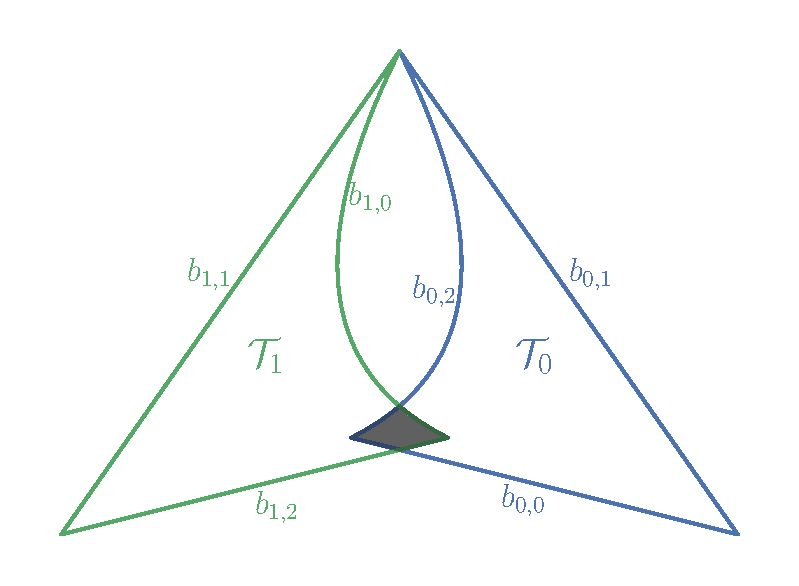
\includegraphics{../images/curved-mesh/main_figure26.pdf}
  \centering
  \captionsetup{width=.75\linewidth}
  \caption{Intersection of B\'{e}zier triangles form a curved polygon.}
  \label{fig:bezier-triangle-intersect}
\end{figure}

When intersecting two curved elements, the resulting surface(s) will
be defined by the boundary, alternating between edges of each
element.
For example, in Figure~\ref{fig:bezier-triangle-intersect}, a
``curved quadrilateral'' is formed when two B\'{e}zier triangles
\(\mathcal{T}_0\) and \(\mathcal{T}_1\) are intersected.

A \textbf{curved polygon} is defined by a collection of B\'{e}zier curves
in \(\reals^2\) that determine the boundary. In order to be
a valid polygon, none of the boundary curves may cross, the
ends of consecutive edge curves must meet and the curves must be right-hand
oriented. For our example in
Figure~\ref{fig:bezier-triangle-intersect}, the triangles
have boundaries formed by three B\'{e}zier curves:
\(\partial \mathcal{T}_0 = b_{0, 0} \cup b_{0, 1} \cup b_{0, 2}\) and
\(\partial \mathcal{T}_1 = b_{1, 0} \cup b_{1, 1} \cup b_{1, 2}\).
The intersection \(\mathcal{P}\) is defined by four boundary
curves: \(\partial \mathcal{P} =
C_1 \cup C_2 \cup C_3 \cup C_4\). Each boundary
curve is itself a B\'{e}zier curve\footnote{A specialization of a
B\'{e}zier curve \(b\left(\left[a_1, a_2\right]\right)\)
is also a B\'{e}zier curve.}:
\(C_1 = b_{0, 0}\left(\left[0, 1/8\right]\right)\),
\(C_2 = b_{1, 2}\left(\left[7/8, 1\right]\right)\),
\(C_3 = b_{1, 0}\left(\left[0, 1/7\right]\right)\) and
\(C_4 = b_{0, 2}\left(\left[6/7, 1\right]\right)\).

Though an intersection can be described in terms of the B\'{e}zier triangles,
the structure of the control net will be lost. The region will not in general
be able to be described by a mapping from a simple space like
\(\utri\).

\section{Error-Free Transformation}

An error-free transformation is a computational method where both
the computed result and the round-off error are returned. It
is considered ``free'' of error if the round-off can be represented
exactly as an element or elements of \(\floats\).
The error-free transformations used in this work are
the \texttt{TwoSum} algorithm by Knuth (\cite{Knuth1997}) and
\texttt{TwoProd} algorithm by Dekker (\cite{Dekker1971}, Section 5),
respectively.

\begin{theorem}[\cite{Ogita2005}, Theorem 3.4]\label{thm:eft}
For \(a, b \in \floats\) and \(P, \pi, S, \sigma \in \floats\),
\texttt{TwoSum} and \texttt{TwoProd} satisfy
\begin{alignat}{4}
\left[S, \sigma\right] &= \mathtt{TwoSum}(a, b), & \, S &= \fl{a + b},
  S + \sigma &= a + b, \sigma &\leq \mach \left|S\right|,
  & \, \sigma &\leq \mach \left|a + b\right| \\
\left[P, \pi\right] &= \mathtt{TwoProd}(a, b),
  & \, P &= \fl{a \times b}, P + \pi &= a \times b,
  \pi &\leq \mach \left|P\right|,
  & \, \pi &\leq \mach \left|a \times b\right|.
\end{alignat}
The letters \(\sigma\) and \(\pi\) are used to indicate that the
errors came from sum and product, respectively. See
Appendix~\ref{chap:appendix-algo} for implementation details.
\end{theorem}

\chapter{B\'{e}zier Intersection Problems}

\section{Intersecting B\'{e}zier Curves}

The problem of intersecting two B\'{e}zier curves is a core building
block for intersecting two B\'{e}zier triangles in \(\mathbf{R}^2\).
Since a curve is a degree one object, the intersections will either
be a curve segment common to both curves (if they coincide) or a finite
set of points.
Many algorithsm have been described in the literature, both
geometric (\cite{Sederberg1986, Sederberg1990, Kim1998}) and
algebraic (\cite{Manocha:CSD-92-698}).

In the implementation for this paper, the B\'{e}zier subdivision
algorithm is used.
In the case of a transversal intersection (i.e. one where the
tangents to each curve are not parallel and both are non-zero),
this algorithm performs very well. However, when curves are tangent,
a large number of (false) candidate intersections are detected and
convergence of Newton's method slows once in a neighborhood of an
actual intersection. Non-transversal intersections
have infinite condition number, but transversal intersections with
very high condition number can also cause convergence problems.

\begin{figure}
  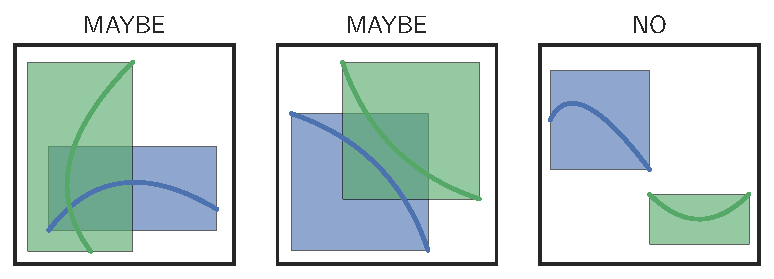
\includegraphics[width=0.9375\textwidth]{../images/curved-mesh/bbox_check.pdf}
  \centering
  \caption{Bounding box check.}
  \label{fig:bounding-box-check}
\end{figure}

In the the B\'{e}zier subdivision algorithm, we first check if the
bounding boxes for the curves are disjoint
(Figure~\ref{fig:bounding-box-check}). We use the bounding boxes
rather than the convex hulls since they are easier to compute and
the intersections of boxes are easier to check.
If they are disjoint, the pair can be rejected. If not, each curve
\(\mathcal{C} = b\left(\left[0, 1\right]\right)\) is split into two halves
by splitting the unit interval \(b\left(\left[0, \frac{1}{2}\right]\right)\)
and \(b\left(\left[\frac{1}{2}, 1\right]\right)\)
(Figure~\ref{fig:bezier-curve-subdivision}). As the subdivision continues,
some pairs of curve segments may be kept around that won't lead to an
intersection (Figure~\ref{fig:bezier-subdivision-process}).
Once the curve segments are close to linear within a given tolerance
(Figure~\ref{fig:bezier-subdivision-linearized}), the process
terminates.

\begin{figure}
  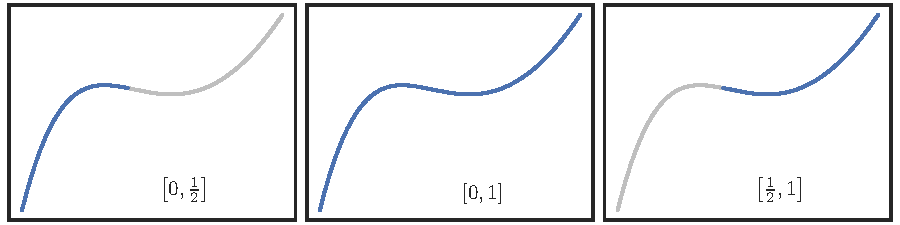
\includegraphics[width=0.9375\textwidth]{../images/curved-mesh/subdivide_curve.pdf}
  \centering
  \caption{B\'{e}zier curve subdivision.}
  \label{fig:bezier-curve-subdivision}
\end{figure}

\begin{figure}
  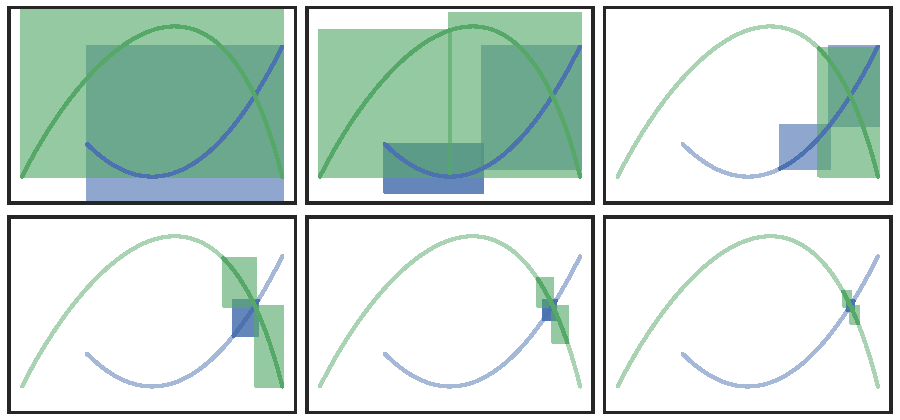
\includegraphics[width=0.9375\textwidth]{../images/curved-mesh/subdivision_process.pdf}
  \centering
  \caption{B\'{e}zier subdivision algorithm.}
  \label{fig:bezier-subdivision-process}
\end{figure}

\begin{figure}
  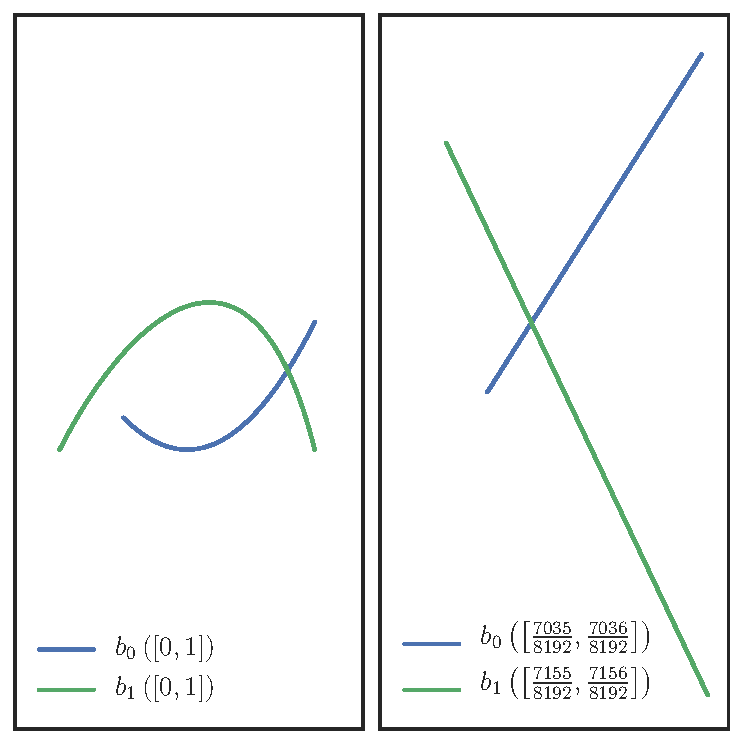
\includegraphics[width=0.96875\textwidth]{../images/curved-mesh/subdivision_linearized.pdf}
  \centering
  \caption{Subdividing until linear within tolerance.}
  \label{fig:bezier-subdivision-linearized}
\end{figure}

\section{Intersecting B\'{e}zier Triangles}

Content.

\section{B\'{e}zier Triangle Inverse}

The problem of determining the parameters \((s, t)\) given a point
\((x, y)\) in a B\'{e}zier triangle...

\chapter{Data Transfer}\label{chap:data-transfer}

\section{Introduction}

In this chapter, an algorithm for conservative data transfer between curved
meshes will be described. This has practical applications to many methods in
computational physics. Data transfer is needed when a solution (approximated
by a discrete field) is known on a \textbf{donor} mesh and must be transferred
to a \textbf{target} mesh. In many applications, the field must be conserved
for physical reasons, e.g. mass or energy cannot leave or enter the system,
hence the focus on \textbf{conservative} data transfer. A few
scenarios where data transfer is necessary will be considered below to
motivate the ``black box'' data transfer algorithm.

Since data transfer is so commonly needed in physical applications, this
problem of conservative interpolation has been considered already for
straight sided meshes. The \textbf{common refinement} approach in
\cite{Jiao2004} is used to compare several methods for data transfer across two
meshes. However, the problem of constructing a common refinement is
not discussed there. The problem of constructing such a refinement is
considered in \cite{Farrell2009, Farrell2011} (called a supermesh by
the authors).
However, the data transfer becomes considerably more challenging for curved
meshes. For a sense of the difference between the straight sided and curved
cases, consider the problem of intersecting an element from the donor mesh
with an element from the target mesh. If the elements are triangles, the
intersection is either a convex polygon or has measure zero. If the elements
are curved, the intersection can be non-convex and can even split into
multiple disjoint regions.

\subsection{Lagrangian Methods}

\begin{figure}
  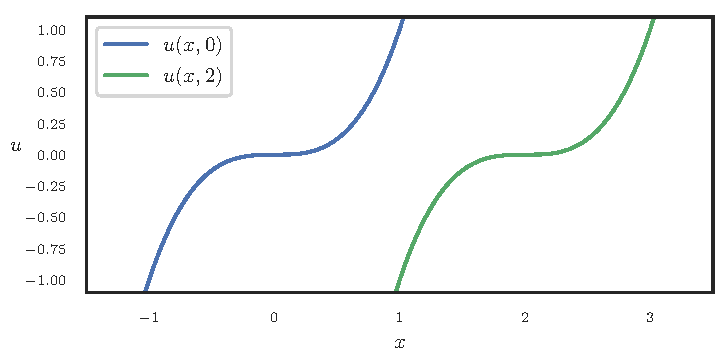
\includegraphics{../images/curved-mesh/simple_transport.pdf}
  \centering
  \captionsetup{width=.75\linewidth}
  \caption{The solution to \(u_t + u_x = 0, \; u(x, 0) = x^3\) plotted in
    the \(xu\)-plane. Demonstrates simple transport of
    the solution.}
  \label{fig:simple-transport}
\end{figure}

The method of characteristics helps transform partial differential equations
into ordinary differential equations by dividing the physical domain into
a family of curves. For example, the simple transport equation
\begin{equation}\label{eq:simple-transport}
u_t + c u_x = 0
\end{equation}
can be transformed when restricting to the family of lines
\(x(t) = x_0 + c t\). On these lines \(u(x(t), t)\) is constant, by
construction, and so the solution is ``transported'' from \(u(x_0, 0)\)
along each characteristic line (Figure~\ref{fig:simple-transport}).

Motivated by this, \textbf{Lagrangian methods} treat each point in the
physical domain as a ``particle'' which moves along a characteristic curve
over time and then monitor values associated with the particle (heat / energy,
velocity, pressure, density, concentration, etc.). They are an effective way
to solve PDEs, even with higher order or non-linear terms.
For example, if a viscosity term is added to~\eqref{eq:simple-transport}
\begin{equation}
u_t + c u_x - \eps u_{xx} = 0
\end{equation}
then the same characteristics can be used, but the value
along each characteristic is no longer constant; instead it satisfies the
ODE \(\frac{d}{dt} u(x(t), t) = \eps u_{xx}\).

This approach transforms the numerical solution of PDEs into a family of
numerical solutions to many independent ODEs. It allows the use of familiar
and well understood ODE solvers. In addition, Lagrangian methods often
have less restrictive conditions on time steps than Eulerian
methods\footnote{In Eulerian methods, the mesh is fixed.}.
When solving PDEs on unstructured meshes
with Lagrangian methods, the nodes move (since they
are treated like particles) and the mesh ``travels''.

\subsection{Remeshing and Adaptivity}

\begin{figure}
  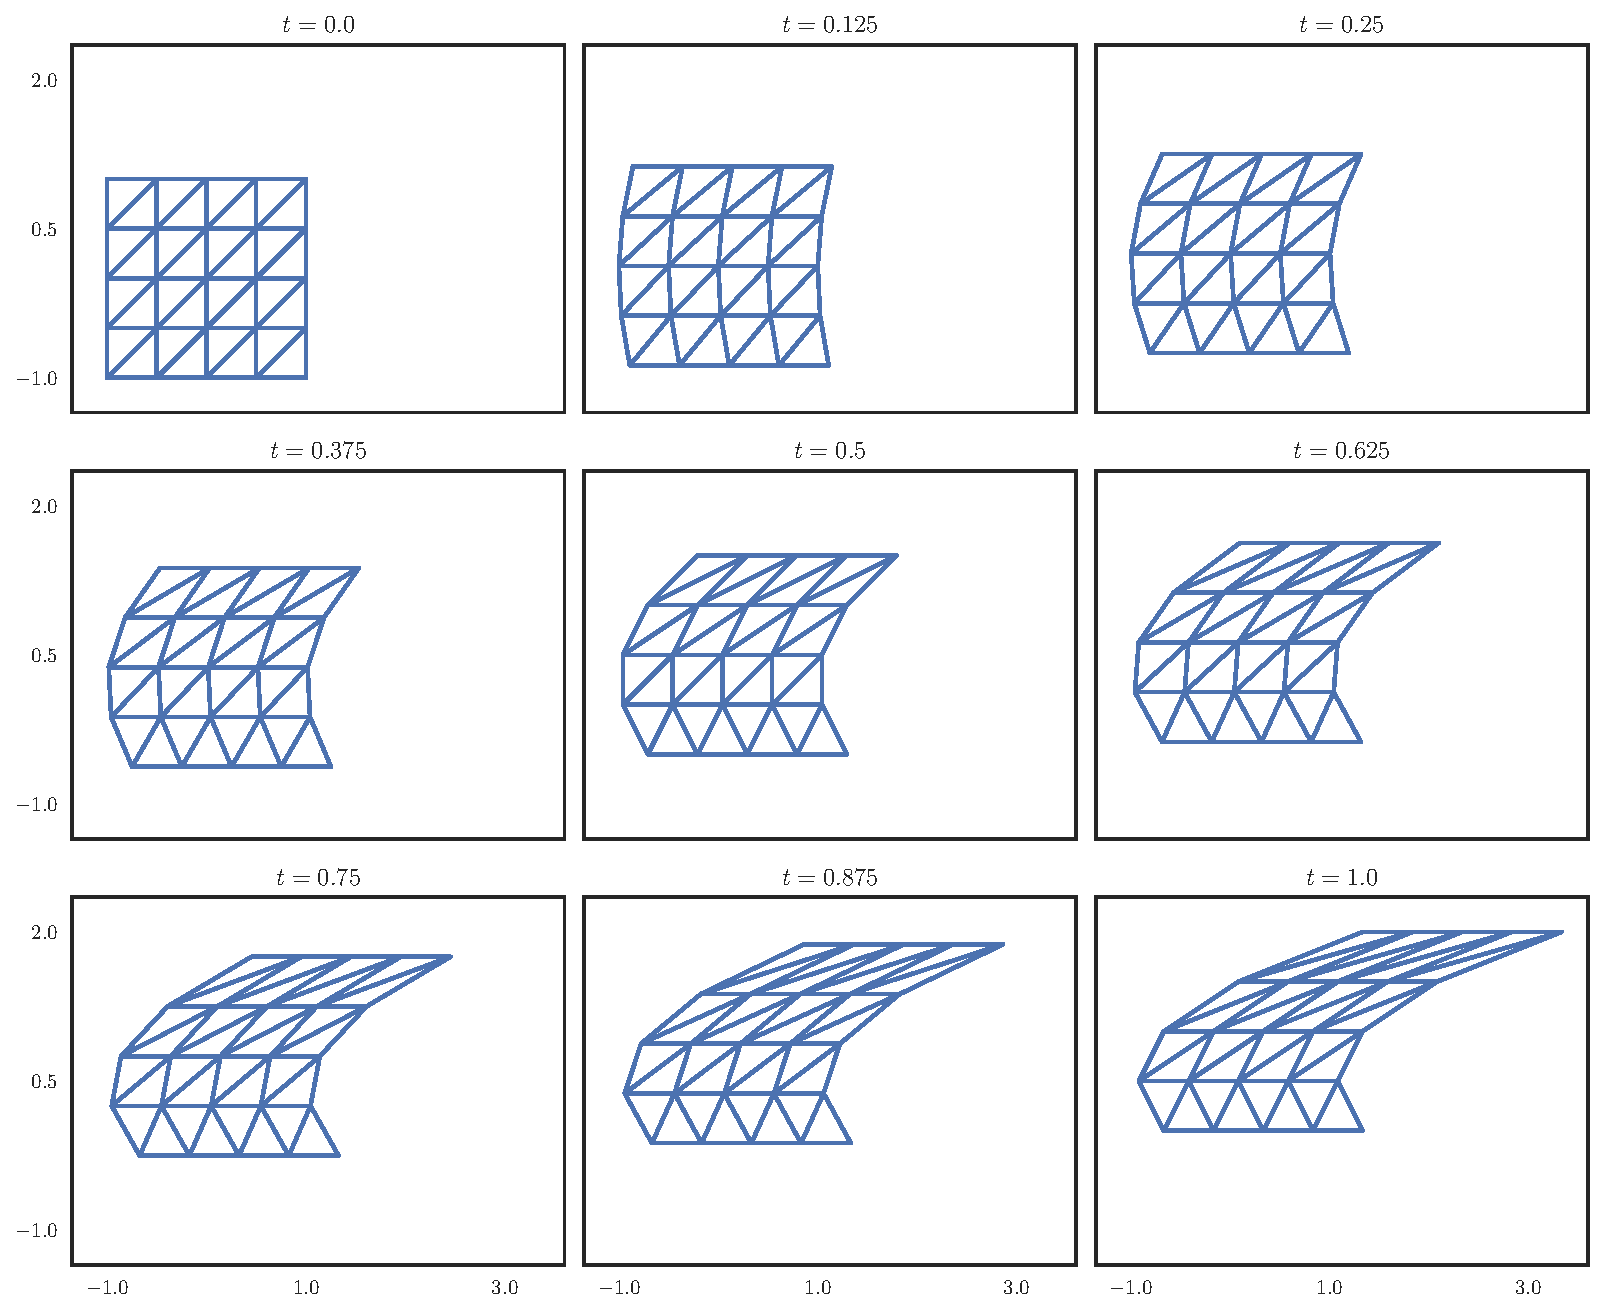
\includegraphics{../images/curved-mesh/mesh_distortion.pdf}
  \centering
  \captionsetup{width=.75\linewidth}
  \caption{Distortion of a regular mesh caused by particle motion along
    the velocity field \(\left[ y^2 \; 1 \right]^T\) from \(t = 0\)
    to \(t = 1\) with \(\Delta t = 1/4\).}
  \label{fig:mesh-distortion}
\end{figure}

A flow-based change to a mesh can cause problems if it causes the mesh to
leave the domain being analyzed or if it distorts the mesh until the element
quality is too low in some mesh elements. Over enough time, the mesh can
even tangle (i.e. elements begin to overlap).
For an example of such distortion (Figure~\ref{fig:mesh-distortion}),
consider a PDE of the form
\begin{equation}\label{eq:non-rigid-characteristics}
u_t + \left[ \begin{array}{c} y^2 \\ 1 \end{array}\right] \cdot \nabla u +
  F\left(u, \nabla u\right) = 0.
\end{equation}
The characteristics \(y(t) = y_0 + t, x(t) = x_0 +
\left(y(t)^3 - y_0^3\right)/3\)
distort the mesh considerably after just one second.

\begin{figure}
  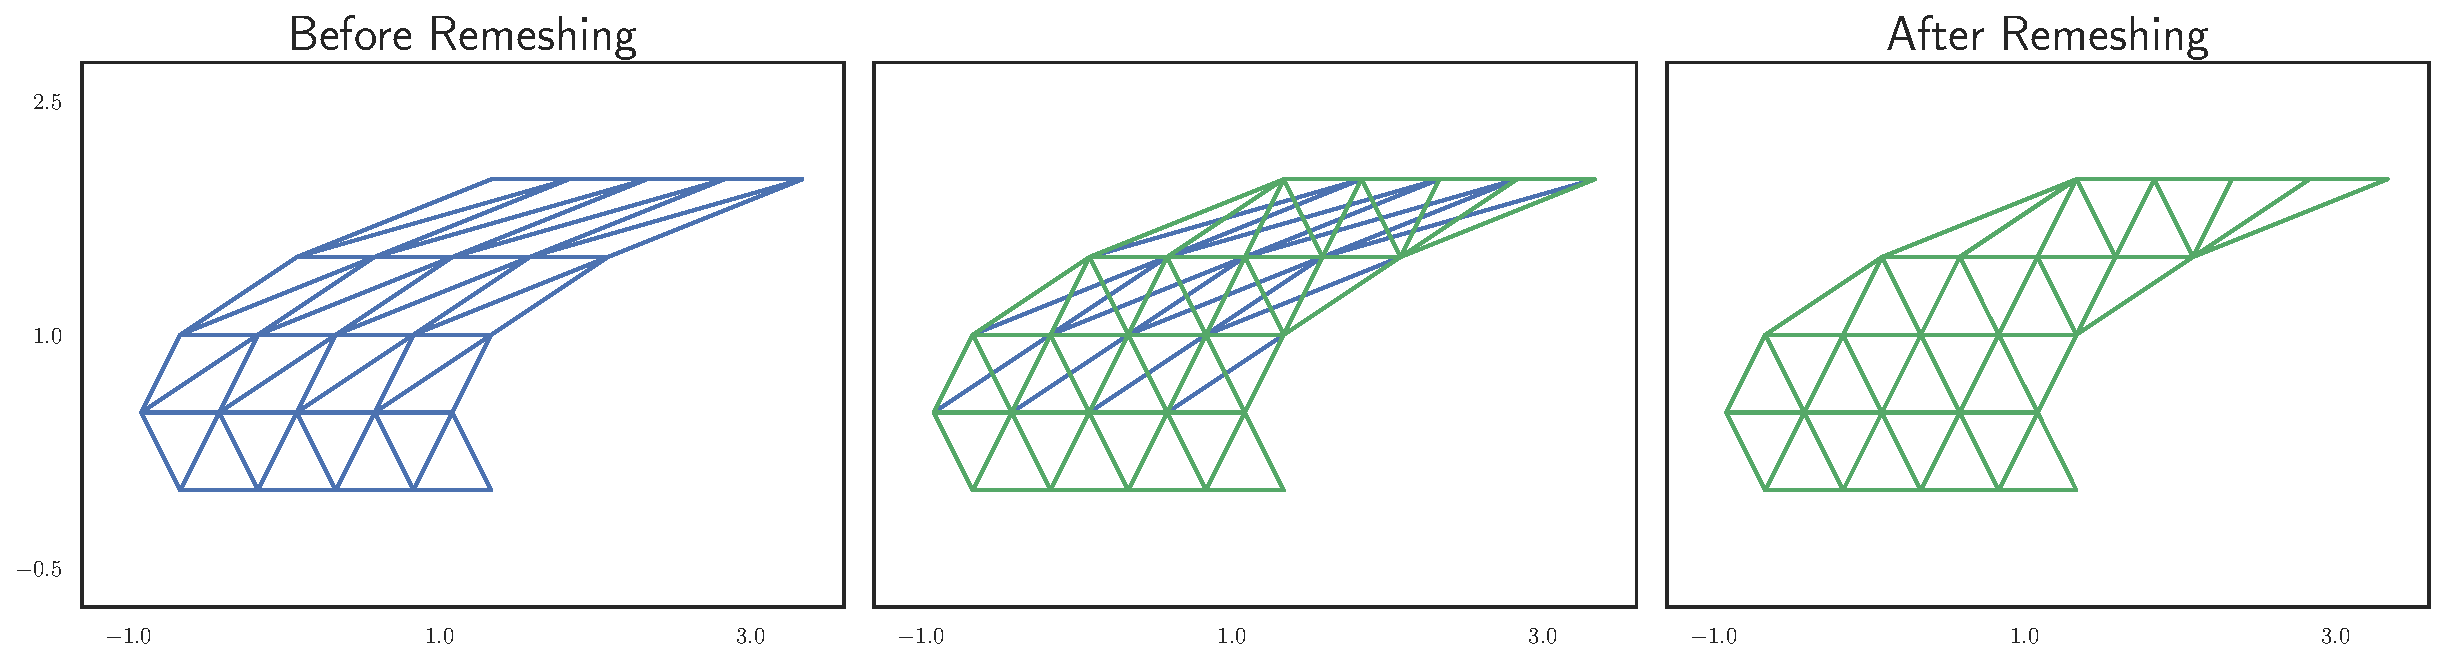
\includegraphics[width=0.9375\textwidth]
                  {../images/curved-mesh/distortion_remesh.pdf}
  \centering
  \captionsetup{width=.75\linewidth}
  \caption{Remeshing a domain after distortion caused by particle motion
    along the velocity field \(\left[ y^2 \; 1 \right]^T\) from \(t = 0\)
    to \(t = 1\).}
  \label{fig:distortion-remesh}
\end{figure}

To deal with distortion, one can allow the mesh to adapt in between time
steps. For example, Figure~\ref{fig:distortion-remesh} shows an example
remeshing of the domain.
In addition to improving mesh quality, mesh
adaptivity can be used to dynamically focus computational effort to resolve
sensitive features of a numerical solution. From~\cite{Iske2004}
\begin{quote}
{\small In order to balance the method's approximation quality and its
computational costs effectively, adaptivity is an essential requirement,
especially when modelling multiscale phenomena.}
\end{quote}
For more on mesh adaptivity, see \cite{Babuska1978, Peraire1987, Pain2001}.

In either case, the change in the
mesh between time steps requires transferring a known solution on the
discarded mesh to the mesh produced by the remeshing process. Without
the ability to change the mesh, Lagrangian methods (or, more generally,
ALE~\cite{Hirt1974}) would not be useful, since after a limited time the
mesh will distort.

\subsection{High-order Meshes}

\begin{figure}
  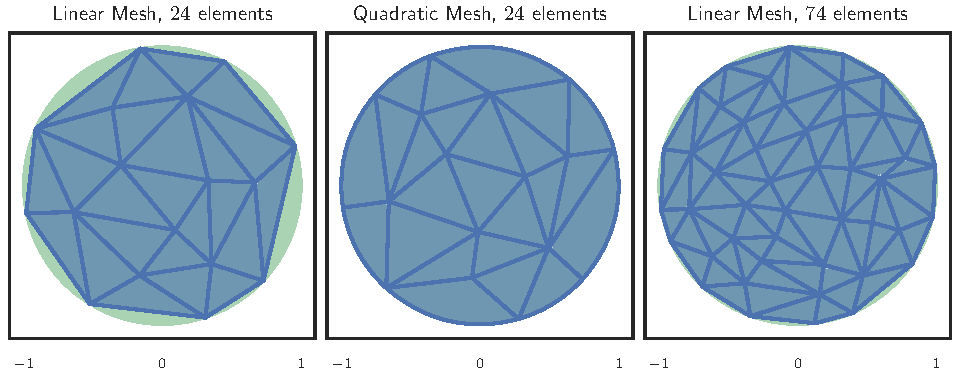
\includegraphics[width=0.9375\textwidth]
                  {../images/curved-mesh/main_figure27.pdf}
  \centering
  \captionsetup{width=.75\linewidth}
  \caption{Comparing straight sided meshes to a curved mesh when approximating
    the unit disc in \(\reals^2\).}
  \label{fig:curved-vs-straight-mesh}
\end{figure}

To allow for greater geometric flexibility and for high order of convergence,
curved mesh elements can be used in the finite element method. Though the
complexity of a method can steeply rise when allowing curved elements, the
trade for high-order convergence can be worth it. (See~\cite{Wang2013} for
more on high-order CFD methods.) Curved meshes can typically
represent a given geometry with far fewer elements than a straight sided mesh
(for example, Figure~\ref{fig:curved-vs-straight-mesh}).
The increase in accuracy also allows for the use of fewer elements, which
in turn can also facilitate a reduction in the overall computation time.

\begin{figure}
  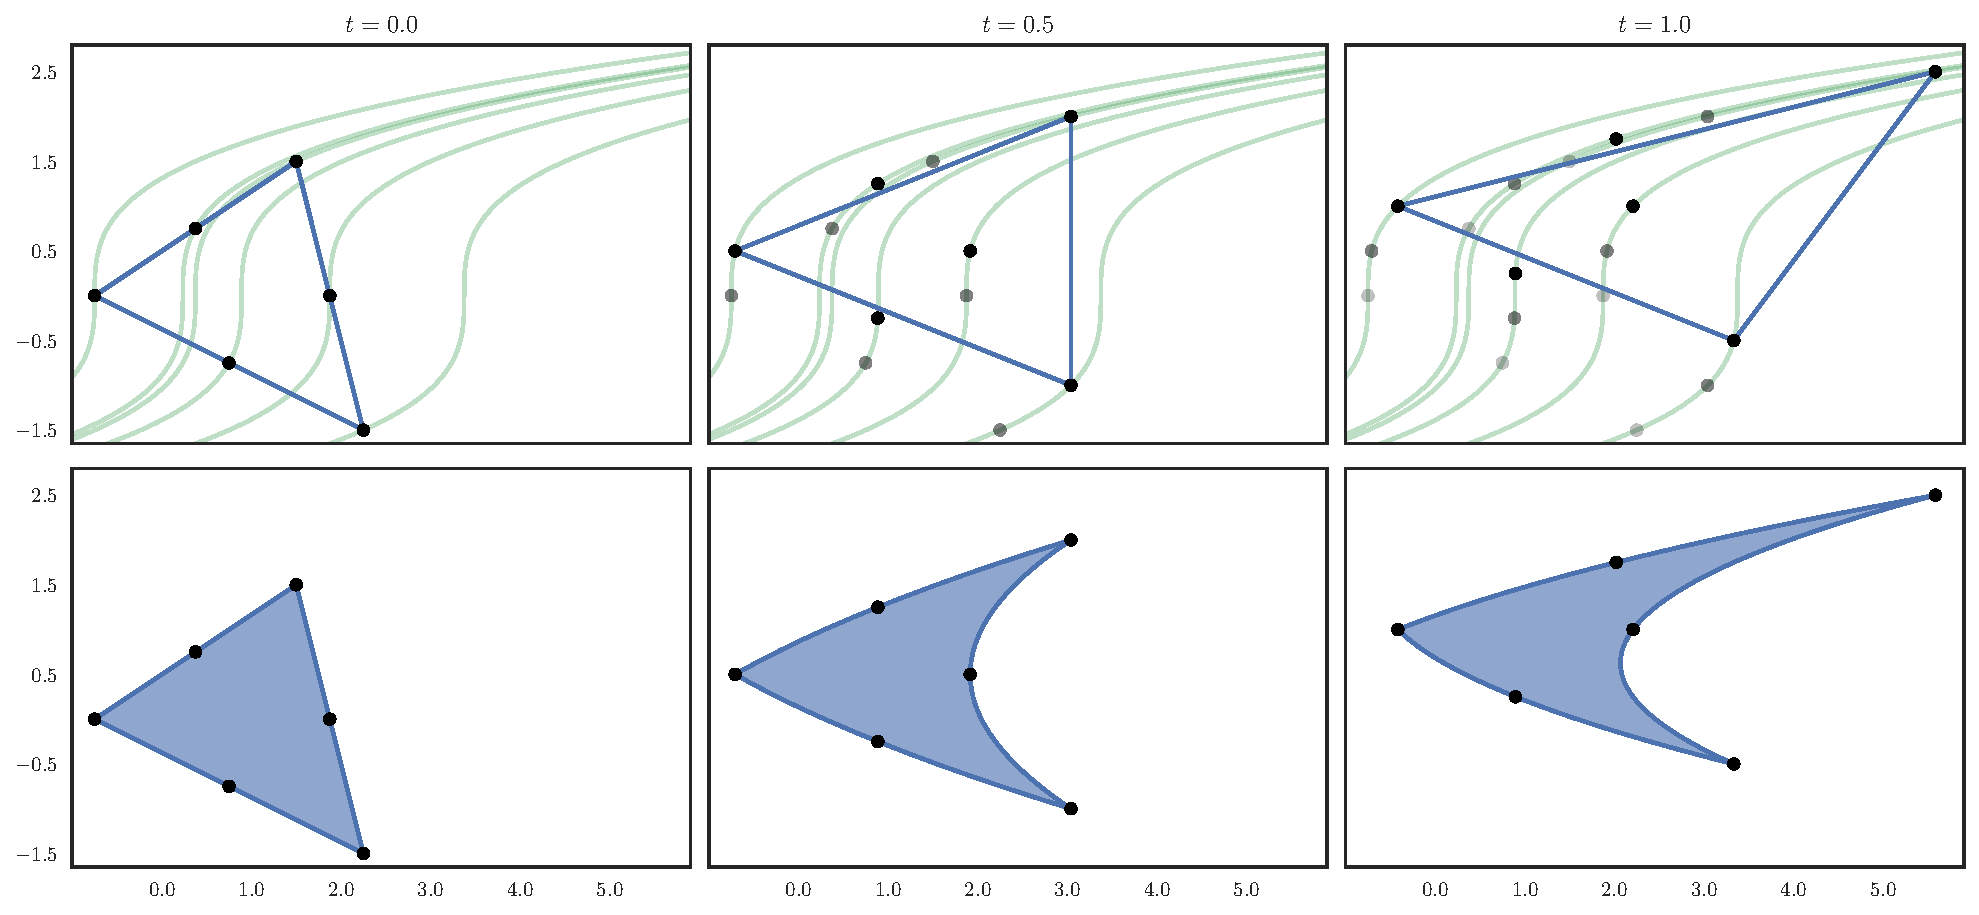
\includegraphics{../images/curved-mesh/element_distortion.pdf}
  \centering
  \captionsetup{width=.75\linewidth}
  \caption{Movement of nodes in a quadratic element under distortion caused
    by particle motion along the velocity field \(\left[ y^2 \; 1 \right]^T\)
    from \(t = 0\) to \(t = 1\) with \(\Delta t = 1/2\). The green curves
    represent the characteristics that each node travels along.}
  \label{fig:element-distortion}
\end{figure}

Even if the domain has no inherent curvature, high-order (degree \(p\)) shape
functions allow for order \(p + 1\) convergence, which is desirable in
it's own right. However, even in such cases, a Lagrangian method must either
curve the mesh or information about the flow of the geometry will be lost.
Figure~\ref{fig:element-distortion} shows what happens to a given
quadratic element as the nodes move along the
characteristics from~\eqref{eq:non-rigid-characteristics}.
This element uses the triangle vertices and edge
midpoints to determine the shape functions. However, as the nodes move
with the flow, the midpoints are no longer on the lines connecting
the vertex nodes. To allow the mesh to more accurately represent the
solution, the edges can instead curve so that the midpoint nodes remain
halfway between (i.e. half of the parameter space) the vertex nodes along
an edge.

%% However, the basis functions of the donor mesh
%% are (in general) discontinuous piecewise polynomials over any given
%% element of the target mesh, which are very difficult to integrate
%% by numerical quadrature schemes.

%% B\'{e}zier curves and triangles were selected for defining
%% mesh elements for two main reasons...
%% Secondly, B\'{e}zier curves and triangles have a
%% number of mathematical properties leading to elegant
%% algorithms.

%% Since adapting the mesh changes the domain for \(\bm{f}\), we
%% must project \(\bm{f}\) onto the new mesh domain. This is
%% accomplished by making local projections of \(\bm{f}\) whenever
%% local mesh modifications are made, and then computing
%% the local reinterpolation error. The choice of a
%% relevant error norm and projection is problem dependent,
%% but the computations are generally easy, since
%% they are done in a local setting with few degrees of
%% freedom. If the calculated re-interpolation error due
%% to a mesh modification is too great, then the modification
%% can be aborted and can be replaced with a mesh
%% refinement.

\subsection{Multiphysics and Comparing Methods}

In multiphysics simulations, a problem is partitioned into physical components.
This partitioning can apply to both the physical domain (e.g. separating a
solid and fluid at an interface) and the simulation data itself (e.g. solving
for pressure on one mesh and velocity on another). Each (multi-)physics
component is solved for on its own mesh. When the components interact, the
simulation data must be transferred between those meshes.

In a similar category of application, data transfer enables the comparison
of solutions defined on different meshes. For example, if a reference
solution is known on a very fine special-purpose mesh, the error can be
computed for a coarse mesh by transferring the solution from the fine
mesh and taking the difference. Or, if the same method is used on
different meshes of the same domain, the resulting computed solutions can
be compared via data transfer. Or, if two different methods use two
different meshes of the same domain.

\subsection{Local versus Global Transfer}

Conservative data transfer has been around since the advent of ALE,
and as a result much of the existing literature focuses on mesh-mesh
pairs that will occur during an ALE-based simulation. When flow-based
mesh distortion occurs, elements are typically ``flipped'' (e.g. a
diagonal is switched in a pair of elements) or elements are subdivided
or combined. These operations are inherently local, hence the data
transfer can be done locally across known neighbors. Typically, this
locality is crucial to data transfer methods. In \cite{Margolin2003},
the transfer is based on partitioning cells of the updated mesh into
components of elements from the old mesh and ``swept regions'' from
neighbouring elements. In \cite{Kucharik2008}, the (locally) changing
connectivity of the mesh is addressed. In \cite{Garimella2007}, the
local transfer is done on polyhedral meshes.

Global data transfer instead seeks to conserve the solution across
the whole mesh. It makes no assumptions about the relationship between
the donor and target meshes. The loss in local information makes
the mesh intersection problem more computationally expensive, but the
added flexibility reduces timestep restrictions since it allows remeshing
to be done less often. In \cite{Dukowicz1984, Dukowicz1987}, a global
transfer is enabled by transforming volume integrals to surface integrals
via the divergence theorem to reduce the complexity of the problem.

\subsection{Limitations}

\begin{figure}
  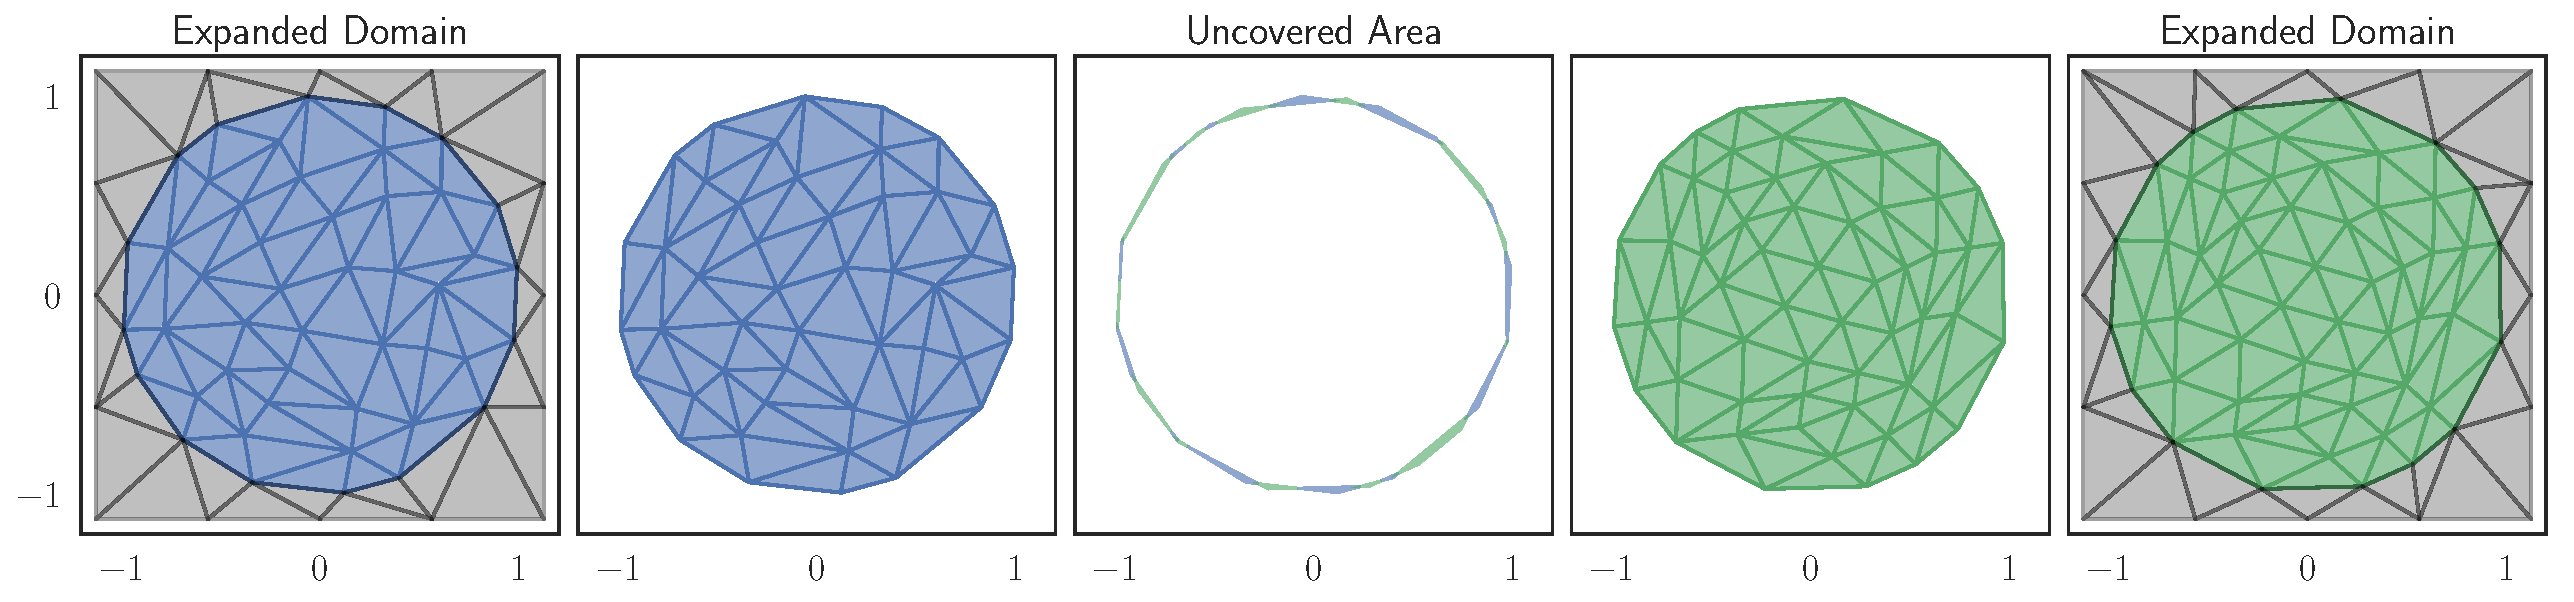
\includegraphics[width=0.96875\textwidth]
                  {../images/curved-mesh/main_figure29.pdf}
  \centering
  \captionsetup{width=.75\linewidth}
  \caption{Partially overlapping meshes on a near identical domain. Both are
    linear meshes that approximate the unit disc in \(\reals^2\). The outermost
    columns show how the domain of each mesh can be expanded so they agree.}
  \label{fig:partially-overlapping}
\end{figure}

The method described in this work only applies to meshes in \(\reals^2\).
Application to meshes in \(\reals^3\) is a direction for future research,
though the geometric kernels (see Chapter~\ref{chap:bezier-intersection})
become significantly more challenging to describe and implement. In
addition, the method will assume that every element in the
target mesh is contained in the donor mesh. This ensures that the data
transfer is \textit{interpolation}. In the case where all target elements are
partially covered, \textit{extrapolation} could be used to extend a solution
outside the domain, but for totally uncovered elements there is no clear
correspondence to elements in the donor mesh.

The case of partially overlapping meshes can be addressed in particular
cases (i.e. with more information). For example, consider a problem
defined on \(\Omega = \reals^2\) and solution
that tends towards zero as points tend to infinity. A typical approach
may be to compute the solution on a circle of large enough radius and
consider the numerical solution to be zero outside the circle.
Figure~\ref{fig:partially-overlapping} shows how data transfer could be
performed in such cases when the meshes partially overlap: construct a
simple region containing both computational domains and then mesh the
newly introduced area. However, the assumption that the numerical solution
is zero in the newly introduced area is very specific and
a similar approach may not apply in other cases of partial overlap.

Some attempts (\cite{Berger1987, Chesshire1994, Cai1999}) have been
made to interpolate fluxes between overlapping meshes. These perform
an interpolation on the region common to both meshes and then numerically
solve the PDE to determine the values on the uncovered elements.

\section{Galerkin Projection}

\begin{figure}
  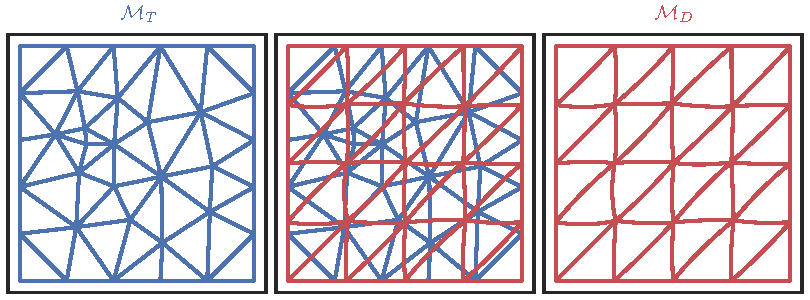
\includegraphics[width=0.8125\textwidth]
                  {../images/curved-mesh/main_figure00.pdf}
  \centering
  \captionsetup{width=.75\linewidth}
  \caption{Mesh pair: donor mesh \(\mathcal{M}_D\) and
    target mesh \(\mathcal{M}_T\).}
  \label{fig:donor-target-pair}
\end{figure}

Consider a donor mesh \(\mathcal{M}_D\) with shape function basis
\(\phi_D^{(j)}\) and a known field \(\bm{q}_D = \sum_j d_j \phi_D^{(j)}\) and a
target mesh \(\mathcal{M}_T\) with shape function basis \(\phi_T^{(j)}\)
(Figure~\ref{fig:donor-target-pair}).
Each shape function \(\phi\) corresponds to a
given isoparametric curved element (see Section~\ref{sec:curved-elements})
\(\mathcal{T}\) in one of these meshes and has
\(\operatorname{supp}(\phi) = \mathcal{T}\).
Additionally, the shape functions are polynomial degree \(p\) (see
Section~\ref{subsec:shape-functions} for a discussion of shape functions),
but the degree of the donor mesh need not be the same as that of the
target mesh. We assume that both meshes cover the same domain \(\Omega \subset
\reals^2\), however we really only require the donor mesh to cover the
target mesh.

We seek the \(L_2\)-optimal interpolant \(\bm{q}_T = \sum_j t_j \phi_T^{(j)}\):
\begin{equation}
\left \lVert \bm{q}_T - \bm{q}_D \right \rVert_2 =
\min_{\bm{q} \in \mathcal{V}_T}
\left \lVert \bm{q} - \bm{q}_D \right \rVert_2
\end{equation}
where \(\mathcal{V}_T = \operatorname{Span}_j\left\{\phi_T^{(j)}\right\}\)
is the function space defined on the target mesh. Since this is optimal in
the \(L_2\) sense, by differentiating with respect to each \(t_j\) in
\(\bm{q}_T\) we find the weak form:
\begin{equation}
\int_{\Omega} \bm{q}_D \phi_T^{(j)} \, dV =
  \int_{\Omega} \bm{q}_T \phi_T^{(j)} \, dV, \qquad \text{for all} j.
\end{equation}
If the constant function \(1\) is contained in \(\mathcal{V}_T\),
conservation follows from the weak form and linearity of the integral
\begin{equation}
\int_{\Omega} \bm{q}_D \, dV =
  \int_{\Omega} \bm{q}_T \, dV.
\end{equation}
Expanding \(\bm{q}_D\) and \(\bm{q}_T\) with respect to their coefficients
\(\bm{d}\) and \(\bm{t}\), the weak form gives rise to a linear system
\begin{equation}\label{eq:weak-form-system}
M_T \bm{t} = M_{TD} \bm{d}.
\end{equation}
Here \(M_T\) is the mass matrix for
\(\mathcal{M}_T\) given by
\begin{equation}
\left(M_T\right)_{ij} = \int_{\Omega} \phi_T^{(i)} \phi_T^{(j)} \, dV.
\end{equation}
In the discontinuous Galerkin case, \(M_T\) is block diagonal with blocks
that correspond to each element, so \eqref{eq:weak-form-system} can be
solved locally on each element \(\mathcal{T}\) in the target mesh. By
construction, \(M_T\) is symmetric and sparse since \(\left(M_T\right)_{ij}\)
will be \(0\) unless \(\phi_T^{(i)}\) and \(\phi_T^{(j)}\) are supported
on the same element \(\mathcal{T}\). In the continuous case, \(M_T\) is
globally coupled since coefficients corresponding to boundary nodes interact
with multiple elements. The matrix \(M_{TD}\) is a ``mixed'' mass matrix
between the target and donor meshes:
\begin{equation}
\left(M_{TD}\right)_{ij} = \int_{\Omega} \phi_T^{(i)} \phi_D^{(j)} \, dV.
\end{equation}
Though boundary conditions can be imposed on the system by fixing boundary
values, this is equivalent to removing some of the basis functions which may
in term make the projection non-conservative. This is because the removed
basis functions may have been used in \(1 = \sum_j u_j \phi_{T}^{(j)}\).

Computing \(M_T\) is fairly straightforward since the (bidirectional) mapping
from elements \(\mathcal{T}\) to basis functions \(\phi_T^{(j)}\) supported
on those elements is known. When using shape functions in the
global coordinates basis (see Section~\ref{subsec:shape-functions}), the
integrand \(F = \phi_T^{(i)} \phi_T^{(j)}\) will be a polynomial of degree
\(2p\) on \(\reals^2\). The domain of integration \(\mathcal{T}
= b\left(\utri\right)\) is the image of a (degree \(p\)) map \(b(s, t)\)
from the unit triangle. Using substitution
\begin{equation}
\int_{b\left(\utri\right)} F(x, y) \, dx \, dy =
  \int_{\utri} \det(Db) F\left(x(s, t), y(s, t)\right) \, ds \, dt
\end{equation}
(we know the map preserves orientation, i.e. \(\det(Db)\) is positive).
Once transformed this way, a quadrature rule on the unit
triangle (\cite{Dunavant1985}) can be used.

On the other hand, computing \(M_{TD}\) is significantly more
challenging. This requires solving both a geometric problem ---
finding the region to integrate over --- and an analytic
problem --- computing the integrals. The integration can be done with
a quadrature rule, though finding this region is significantly
more difficult.

\section{Common Refinement}

\begin{figure}
  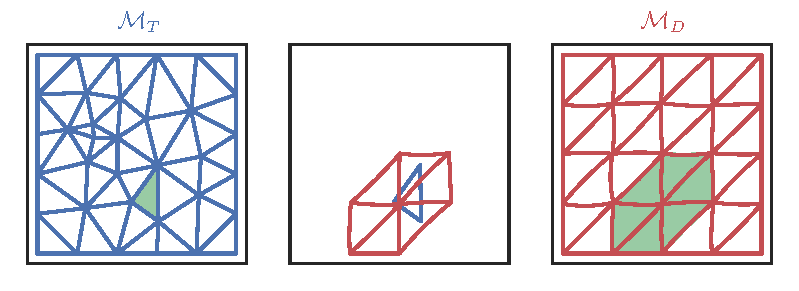
\includegraphics[width=0.8125\textwidth]
                  {../images/curved-mesh/main_figure02.pdf}
  \centering
  \captionsetup{width=.75\linewidth}
  \caption{All donor elements that cover a target element}
  \label{fig:target-elt-all-matching}
\end{figure}

Rather than computing \(M_{TD}\), the right-hand side
of~\eqref{eq:weak-form-system} can be computed directly via
\begin{equation}\label{eq:lumped-mixed-mass-matrix}
\left(M_{TD} \bm{d}\right)_j = \int_{\Omega} \phi_T^{(j)} \bm{q}_D \, dV.
\end{equation}
Any given \(\phi\) is supported on an element \(\mathcal{T}\) in the
target mesh. Since \(\bm{q}_D\) is piecewise defined over each element
\(\mathcal{T}'\) in the donor mesh, the
integral~\eqref{eq:lumped-mixed-mass-matrix} may be problematic.
In the continuous Galerkin case, \(\bm{q}_D\) need not be differentiable
across \(\mathcal{T}\) and in the discontinuous Galerkin case,
\(\bm{q}_D\) need not even be continuous. This necessitates a
partitioning of the domain:
\begin{equation}
\int_{\Omega} \phi \, \bm{q}_D \, dV =
  \int_{\mathcal{T}} \phi \, \bm{q}_D \, dV =
  \sum_{\mathcal{T}' \in \mathcal{M}_D} \int_{\mathcal{T} \cap \mathcal{T}'}
    \phi \left.\bm{q}_D\right|_{\mathcal{T}'} \, dV.
\end{equation}
In other words, the integral over \(\mathcal{T}\) splits into integrals
over intersections \(\mathcal{T} \cap \mathcal{T}'\) for all
\(\mathcal{T}'\) in the donor mesh that intersect \(\mathcal{T}\)
(Figure~\ref{fig:target-elt-all-matching}).

\subsection{Curved versus Polygonal Computing}

\begin{figure}
  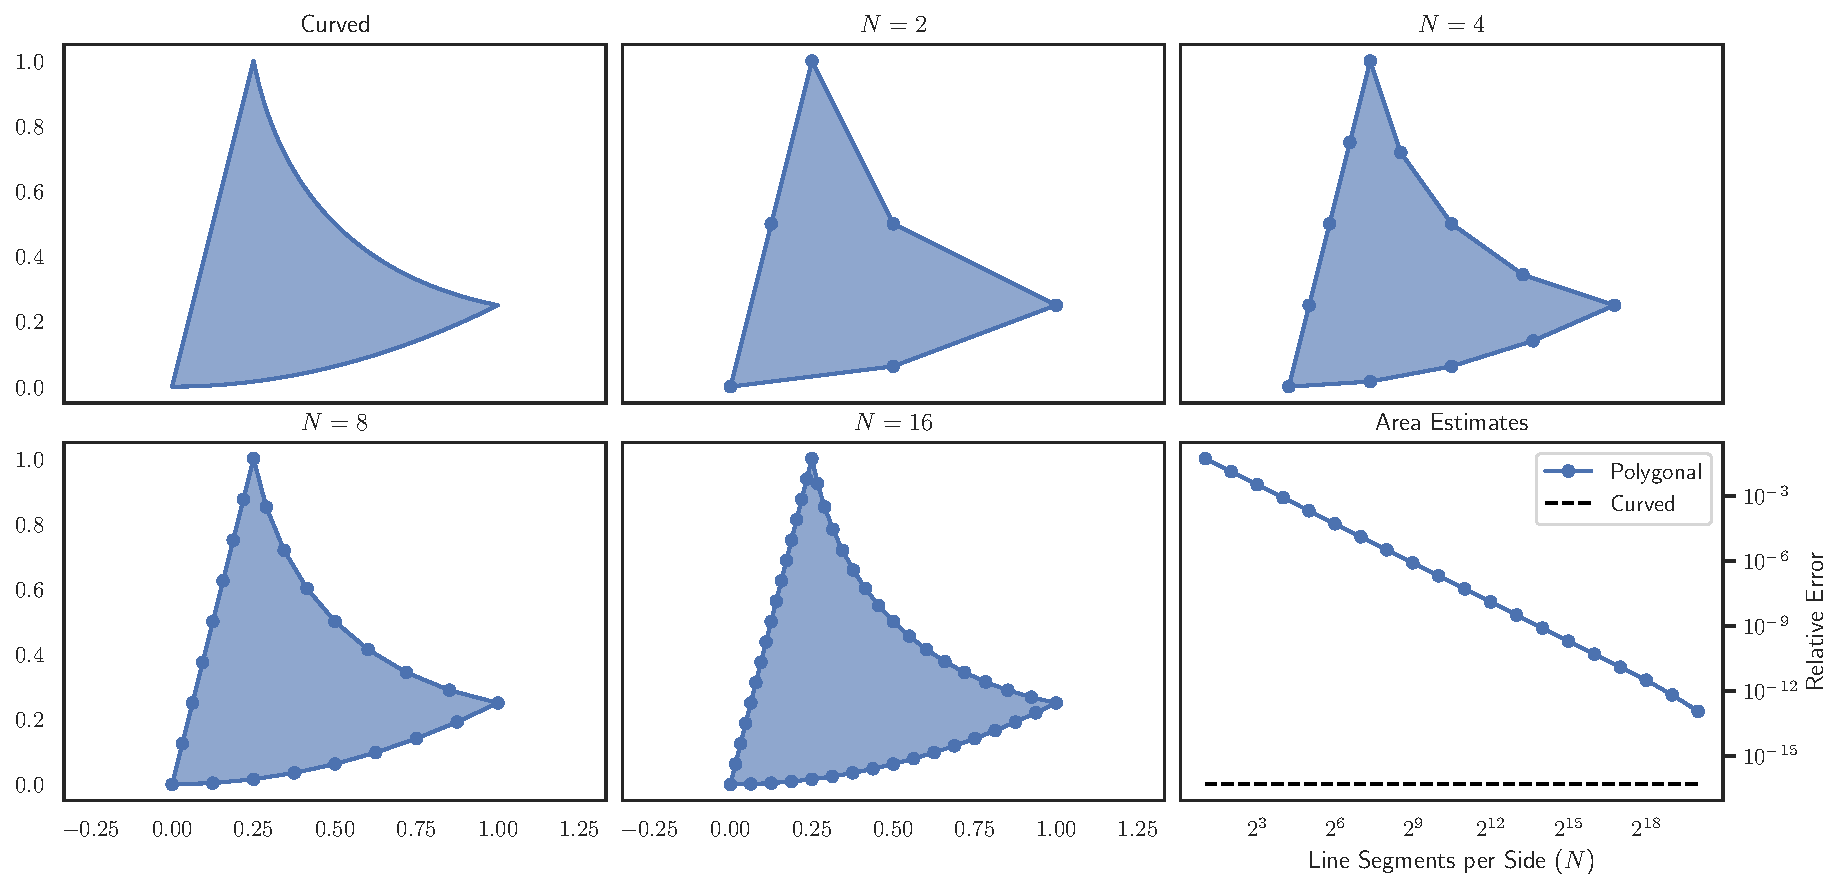
\includegraphics[width=0.9375\textwidth]
                  {../images/curved-mesh/polygon_vs_curved.pdf}
  \centering
  \captionsetup{width=.75\linewidth}
  \caption{Comparing the relative error for the computed area of a quadratic
    B\'{e}zier triangle. In one method, the curved boundary is used with
    Green's method and it is correct to machine precision. In the other,
    the curved edges are approximated by polygonal paths. These paths are
    generated from equally spaced parameters, for example a B\'{e}zier curve
    \(b(s)\) with \(N = 4\) would be approximated by a line connecting
    \(b(0), b(1/4), b(1/2), b(3/4)\) and \(b(1)\).}
  \label{fig:polygon-vs-curved}
\end{figure}

\begin{figure}
  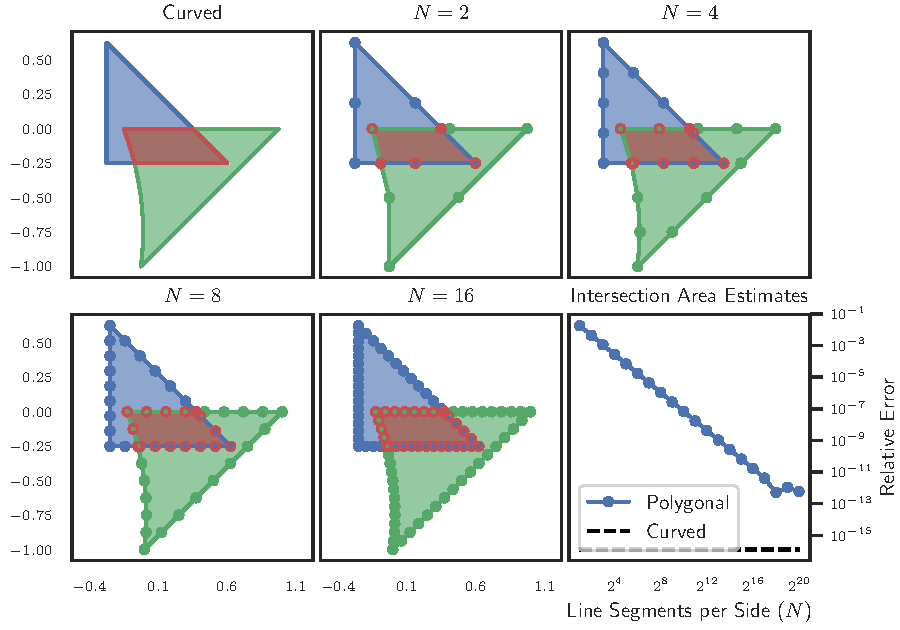
\includegraphics[width=0.9375\textwidth]
                  {../images/curved-mesh/polygon_vs_curved_intersection.pdf}
  \centering
  \captionsetup{width=.75\linewidth}
  \caption{Comparing the relative error for the computed area of the
    intersection of two quadratic B\'{e}zier triangles. In one method, the
    intersection boundary is fully specified as the union of B\'{e}zier curve
    segments and the area is found via Green's method. This method is correct
    to machine precision. In the other, the curved edges are approximated by
    polygonal paths and the intersection of the resulting polygons is computed.
    These paths are generated from equally spaced parameters, for example a
    B\'{e}zier curve \(b(s)\) with \(N = 4\) would be approximated by a line
    connecting \(b(0), b(1/4), b(1/2), b(3/4)\) and \(b(1)\).}
  \label{fig:polygon-vs-curved-intersection}
\end{figure}

\chapter{Compensated de Casteljau algorithm in \(K\) times the
  working precision}

\section{Introduction}

In computer aided geometric design, polynomials are usually expressed in
Bernstein form. Polynomials in this form are usually evaluated by the
de Casteljau algorithm. This algorithm has a round-off error bound
which grows only linearly with degree, even though the number of
arithmetic operations grows quadratically. The Bernstein basis is
optimally suited (\cite{Farouki1987, Delgado2015, Mainar2005})
for polynomial evaluation; it is
typically more accurate than the monomial basis, for example in
Figure~\ref{fig:horner-inferior} evaluation via Horner's method produces
a jagged curve for points near a triple root, but the de Casteljau algorithm
produces a smooth curve. Nevertheless the de Casteljau
algorithm returns results arbitrarily less accurate than the working
precision \(\mach\) when evaluating \(p(s)\) is ill-conditioned.
The relative accuracy of the computed
evaluation with the de Casteljau algorithm (\texttt{DeCasteljau}) satisfies
(\cite{Mainar1999}) the following a priori bound:
\begin{equation}\label{de-casteljau-error}
  \frac{\left|p(s) - \mathtt{DeCasteljau}(p, s)\right|}{\left|p(s)\right|} \leq
  \cond{p, s} \times \bigO{\mach}.
\end{equation}
In the right-hand side of this inequality, \(\mach\) is the computing
precision and the condition number \(\cond{p, s} \geq 1\) only depends
on \(s\) and the Bernstein coefficients of \(p\) --- its expression will
be given further.

\begin{figure}
  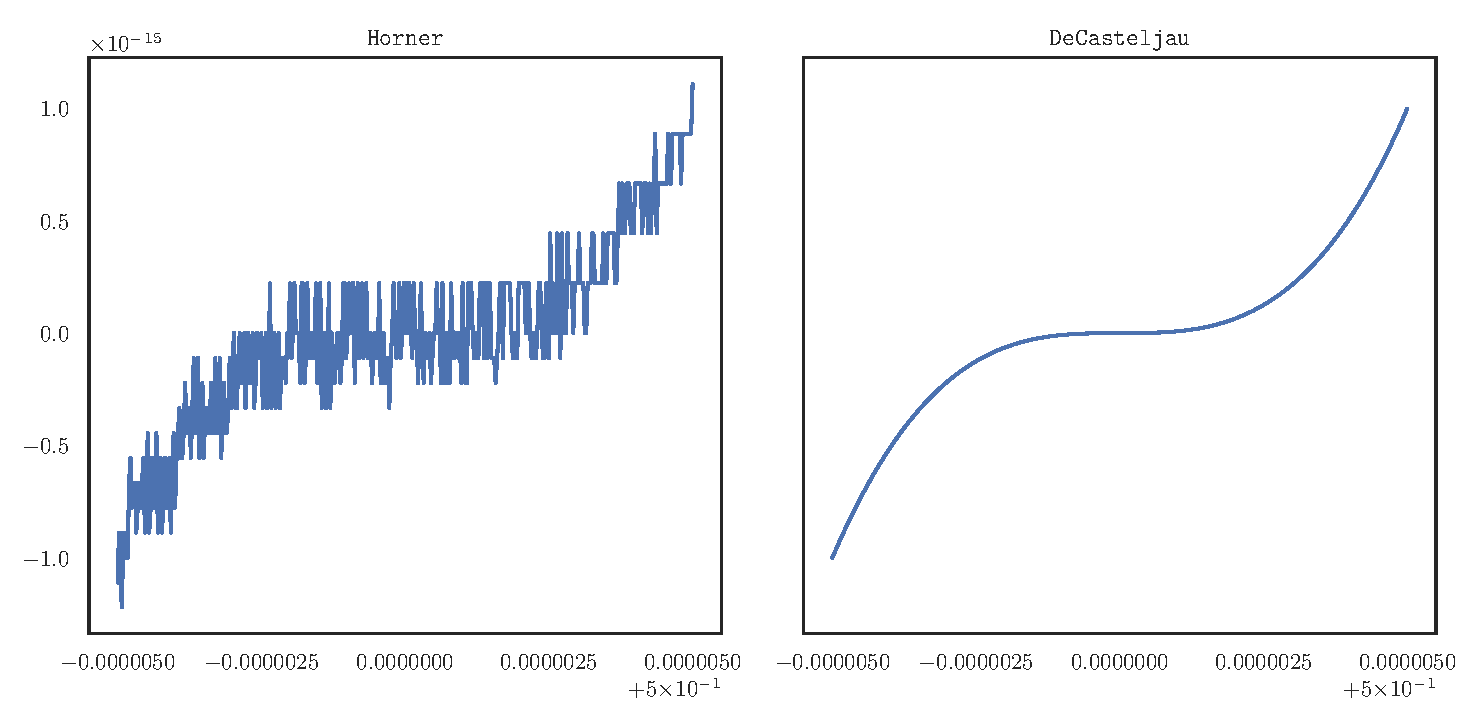
\includegraphics[width=0.9375\textwidth]{../images/k-compensated/horner_inferior.pdf}
  \centering
  \captionsetup{width=.75\linewidth}
  \caption{Comparing Horner's method to the de Casteljau method for
    evaluating \(p(s) = (2s - 1)^3\) in the neighborhood of its
    multiple root \(1/2\).}
  \label{fig:horner-inferior}
\end{figure}

For ill-conditioned problems, such as evaluating \(p(s)\) near a
multiple root, the condition number may be arbitrarily large, i.e.
\(\cond{p, s} > 1 / \mach\), in
which case most or all of the computed digits will be incorrect.
In some cases, even the order of magnitude of the computed value
of \(p(s)\) can be incorrect.

To address ill-conditioned problems, error-free transformations (EFT) can
be applied in \textit{compensated algorithms} to account for round-off.
Error-free transformations were studied in great detail in \cite{Ogita2005}
and open a large number of applications.
In \cite{langlois_et_al:DSP:2006:442}, a compensated Horner's algorithm was
described to evaluate a polynomial in the monomial basis. In \cite{Jiang2010},
a similar method was described to perform a compensated version of the de
Casteljau algorithm. In both cases, the \(\cond{p, s}\) factor is moved
from \(\mach\) to \(\mach^2\) and the computed value is as accurate
as if the computations were done in twice the working precision. For example,
the compensated de Casteljau algorithm (\texttt{CompDeCasteljau}) satisfies
\begin{equation}\label{de-casteljau-2-error}
  \frac{\left|p(s) - \mathtt{CompDeCasteljau}(p, s)\right|}{
    \left|p(s)\right|} \leq \mach + \cond{p, s} \times
    \bigO{\mach^2}.
\end{equation}
For problems with \(\cond{p, s} < 1 / \mach^2\), the relative error
is \(\mach\), i.e. accurate to full precision, aside from rounding to the
nearest floating point number. Figure~\ref{fig:jlcs-10} shows this shift
in relative error from \texttt{DeCasteljau} to \texttt{CompDeCasteljau}.

\begin{figure}
  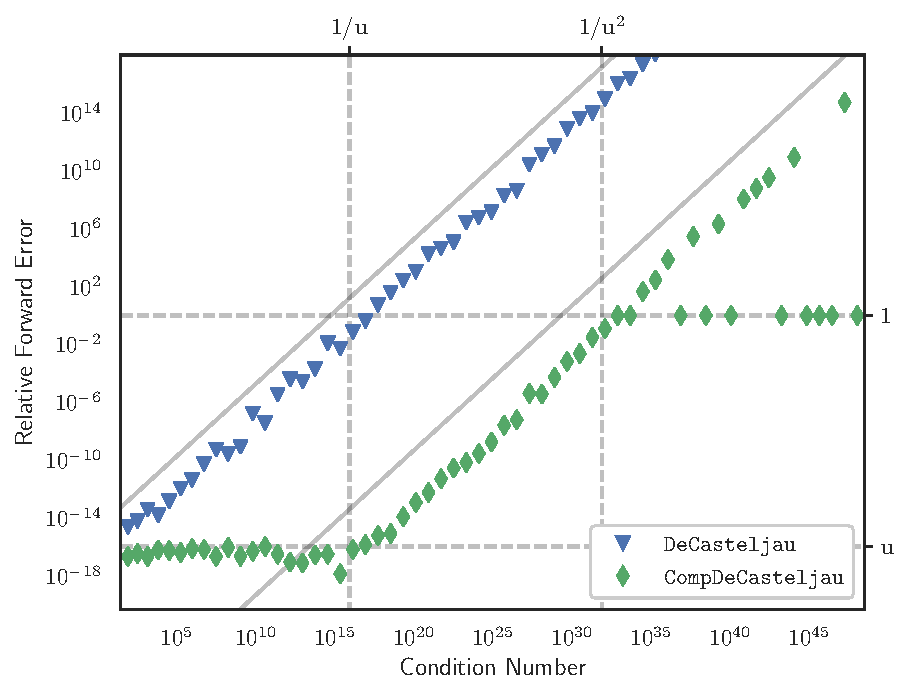
\includegraphics[width=0.8125\textwidth]{../images/k-compensated/jlcs10_plot.pdf}
  \centering
  \captionsetup{width=.75\linewidth}
  \caption{Evaluation of \(p(s) = (s - 1)\left(s - 3/4\right)^7\)
    represented in Bernstein form.}
  \label{fig:jlcs-10}
\end{figure}

In \cite{Graillat2009}, the authors generalized the compensated Horner's
algorithm to produce a method for evaluating a polynomial as if
the computations were done in \(K\) times the working precision for
any \(K \geq 2\). This result motivates this paper, though the
approach there is somewhat different than ours. They perform each computation
with error-free transformations and interpret the errors as coefficients of new
polynomials. They then evaluate the error polynomials, which (recursively)
generate second order error polynomials and so on. This recursive property
causes the number of operations to grow exponentially in \(K\). Here, we
instead have a fixed number of error groups, each corresponding to round-off
from the group above it. For example, when
\((1 - s) b_j^{(n)} + s b_{j + 1}^{(n)}\) is computed in floating point, any
error is filtered down to the error group below it.

As in~\eqref{de-casteljau-error}, the accuracy of the compensated
result~\eqref{de-casteljau-2-error} may be arbitrarily bad for ill-conditioned
polynomial evaluations. For example, as the condition number grows in
Figure~\ref{fig:jlcs-10}, some points have relative error exactly equal to
\(1\); this indicates that \(\mathtt{CompDeCasteljau}(p, s) = 0\), which is
a complete failure to evaluate the order of magnitude of \(p(s)\). For
root-finding problems \(\mathtt{CompDeCasteljau}(p, s) = 0\) when
\(p(s) \neq 0\) can cause premature convergence and incorrect results.
We describe how to defer rounding into progressively
smaller error groups and improve the accuracy of the computed result by a
factor of \(\mach\) for every error group added. So we derive
\texttt{CompDeCasteljauK}, a \(K\)-fold compensated de Casteljau algorithm
that satisfies the following a priori bound for any arbitrary integer \(K\):
\begin{equation}
  \frac{\left|p(s) - \mathtt{CompDeCasteljauK}(p, s, K)\right|}{
    \left|p(s)\right|} \leq \mach + \cond{p, s} \times
    \bigO{\mach^K}.
\end{equation}
This means that the computed value with \texttt{CompDeCasteljauK} is now
as accurate as the result of the de Casteljau algorithm performed in
\(K\) times the working precision with a final rounding back to the
working precision.

The paper is organized as follows. Section~\ref{chap:preliminaries} establishes
notation for error analysis with floating point operations, reviews
results about error-free transformations and reviews the
de Casteljau algorithm. In Section~\ref{sec:compensated-2},
the compensated algorithm for polynomial evaluation from \cite{Jiang2010} is
reviewed and notation is established for the expansion. In
Section~\ref{sec:compensated-k}, the \(K\)-compensated algorithm is provided
and a forward error analysis is performed. Finally, in
Section~\ref{sec:numerical} we perform two numerical experiments to
give practical examples of the theoretical error bounds.

\section{Compensated de Casteljau}\label{sec:compensated-2}

In this section we review the compensated de Casteljau algorithm
from \cite{Jiang2010}. In order to track the local errors at
each update step, we use four EFTs:
\begin{align}
\left[\widehat{r}, \rho\right] &= \mathtt{TwoSum}(1, -s) \\
\left[P_1, \pi_1\right] &= \mathtt{TwoProd}\left(
    \widehat{r}, \widehat{b}_j^{(k + 1)}\right) \\
\left[P_2, \pi_2\right] &= \mathtt{TwoProd}\left(
    s, \widehat{b}_{j + 1}^{(k + 1)}\right) \\
\left[\widehat{b}_j^{(k)}, \sigma_3\right] &= \mathtt{TwoSum}(P_1, P_2)
\end{align}
With these, we can exactly describe the local error between the exact
update and computed update:
\begin{gather}
\ell_{1, j}^{(k)} = \pi_1 + \pi_2 + \sigma_3 + \rho \cdot
  \widehat{b}_j^{(k + 1)} \label{ell-j} \\
(1 - s) \cdot \widehat{b}_j^{(k + 1)} +
  s \cdot \widehat{b}_{j + 1}^{(k + 1)} =
\widehat{b}_j^{(k)} + \ell_{1, j}^{(k)}.
\end{gather}

\begin{figure}
  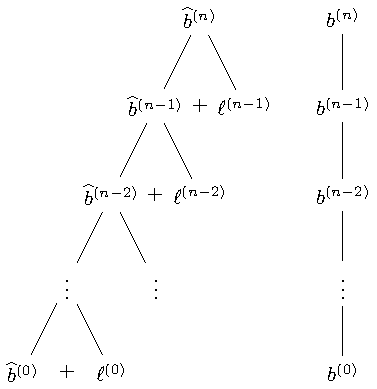
\includegraphics[width=0.375\textwidth]{tikz_local_err.pdf}
  \centering
  \captionsetup{width=.75\linewidth}
  \caption{Local round-off errors}
  \label{fig:loc-err-accumulate}
\end{figure}

\noindent By defining the global errors at each step
\begin{equation}
  \db{1}_j^{(k)} = b_j^{(k)} - \widehat{b}_j^{(k)}
\end{equation}
we can see (Figure~\ref{fig:loc-err-accumulate}) that the local errors
accumulate in
\(\db{1}^{(k)}\):
\begin{equation}\label{err-update}
  \db{1}_j^{(k)} = (1 - s) \cdot \db{1}_j^{(k + 1)} + s \cdot
  \db{1}_{j + 1}^{(k + 1)} + \ell_{1, j}^{(k)}.
\end{equation}
When computed in exact arithmetic
\begin{equation}
  p(s) = \widehat{b}_0^{(0)} + \db{1}_0^{(0)}
\end{equation}
and by using \eqref{err-update}, we can continue to compute
approximations of \(\db{1}_j^{(k)}\). The idea behind the compensated
de Casteljau algorithm is to compute both the local error and the updates
of the global error with floating point operations:

\begin{breakablealgorithm}
  \caption{\textit{Compensated de Casteljau algorithm for polynomial evaluation.}}
  \label{alg:comp-de-casteljau}

  \begin{algorithmic}
    \Function{\(\mathtt{result} = \mathtt{CompDeCasteljau}\)}{$b, s$}
      \State \(n = \texttt{length}(b) - 1\)
      \State \(\left[\widehat{r}, \rho\right] = \mathtt{TwoSum}(1, -s)\)
      \\
      \For{\(j = 0, \ldots, n\)}
        \State \(\widehat{b}_j^{(n)} = b_j\)
        \State \(\cdb{1}_j^{(n)} = 0\)
      \EndFor
      \\
      \For{\(k = n - 1, \ldots, 0\)}
        \For{\(j = 0, \ldots, k\)}
          \State \(\left[P_1, \pi_1\right] = \mathtt{TwoProd}\left(
              \widehat{r}, \widehat{b}_j^{(k + 1)}\right)\)
          \State \(\left[P_2, \pi_2\right] = \mathtt{TwoProd}\left(
              s, \widehat{b}_{j + 1}^{(k + 1)}\right)\)
          \State \(\left[\widehat{b}_j^{(k)}, \sigma_3\right] =
              \mathtt{TwoSum}(P_1, P_2)\)
          \State \(\widehat{\ell}_{1, j}^{(k)} = \pi_1 \oplus \pi_2 \oplus
              \sigma_3 \oplus \left(\rho \otimes
              \widehat{b}_j^{(k + 1)}\right)\)
          \State \(\cdb{1}_j^{(k)} =
              \widehat{\ell}_{1, j}^{(k)} \oplus
              \left(s \otimes \cdb{1}_{j + 1}^{(k + 1)}
              \right) \oplus
              \left(\widehat{r} \otimes
              \cdb{1}_j^{(k + 1)}\right)\)
        \EndFor
      \EndFor
      \\
      \State \(\mathtt{result} = \widehat{b}_0^{(0)} \oplus
          \cdb{1}_0^{(0)}\)
    \EndFunction
  \end{algorithmic}
\end{breakablealgorithm}

\noindent  When comparing this computed error to the exact error, the
difference depends only on \(s\) and the Bernstein
coefficients of \(p\). Using a bound (Lemma~\ref{lemma:db-lemma}) on the
round-off error when computing \(\db{1}^{(0)}\), the algorithm can
be shown to be as accurate as if the computations were done in twice
the working precision:

\begin{theorem}[\cite{Jiang2010}, Theorem 5]
  If no underflow occurs, \(n \geq 2\) and \(s \in \left[0, 1\right]\)
  \begin{equation}
    \frac{\left|p(s) - \mathtt{CompDeCasteljau}(p, s)\right|}{
      \left|p(s)\right|} \leq \mach + 2 \gamma_{3n}^2 \cond{p, s}.
  \end{equation}
\end{theorem}

\begin{figure}
  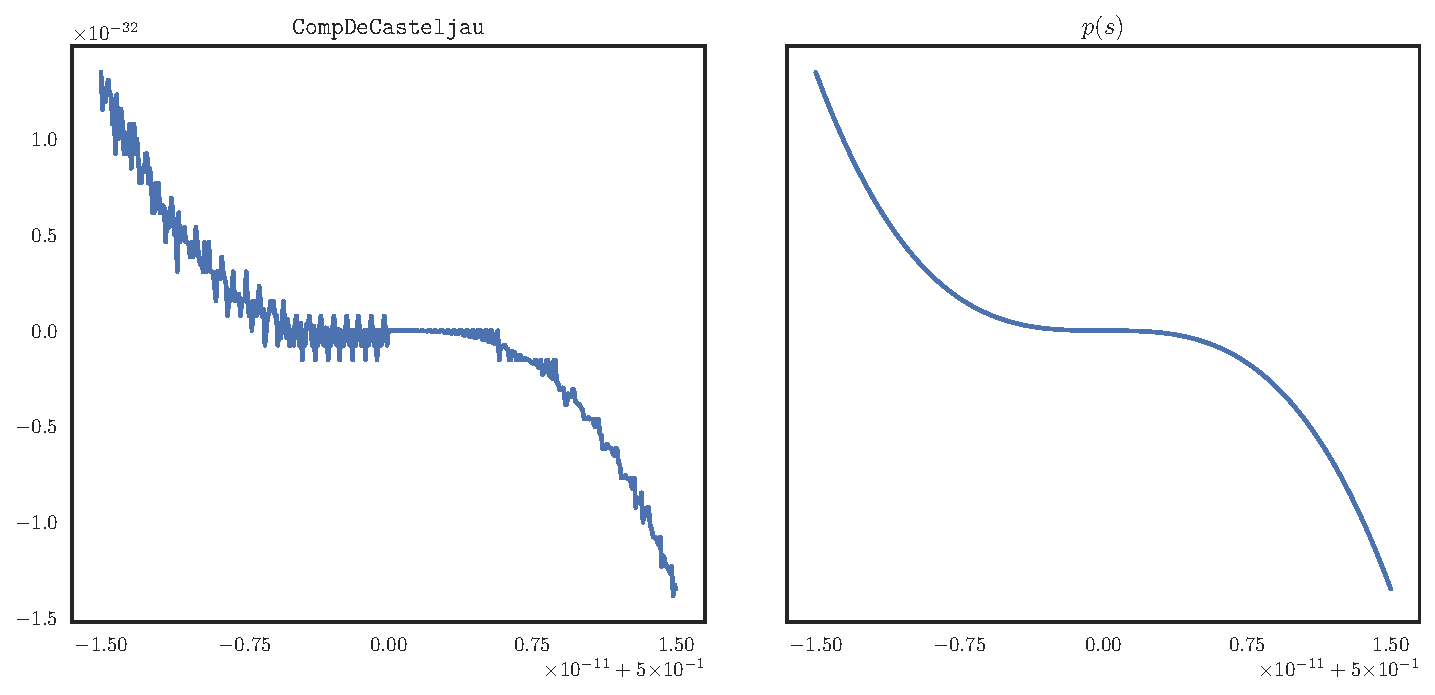
\includegraphics[width=0.9375\textwidth]{../images/k-compensated/compensated_insufficient.pdf}
  \centering
  \captionsetup{width=.75\linewidth}
  \caption{The compensated de Casteljau method starts to lose accuracy
    for \(p(s) = (2s - 1)^3 (s - 1)\) in the neighborhood of its
    multiple root \(1/2\).}
  \label{fig:compensated-insufficient}
\end{figure}

Unfortunately, Figure~\ref{fig:compensated-insufficient} shows how
\texttt{CompDeCasteljau} starts to break down in a region of
high condition number (caused by a multiple root with multiplicity
higher than two). For example, the point
\(s = \frac{1}{2} + 1001\mach\)
--- which is in the plotted region \(\left|s - \frac{1}{2}\right|
\leq \frac{3}{2} \cdot 10^{-11}\) --- evaluates to exactly \(0\) when
it should be \(\bigO{\mach^3}\). As shown in
Table~\ref{tab:exact-computation}, the breakdown occurs because
\(\widehat{b}_0^{(0)} = -\cdb{1}_0^{(0)} = \mach / 16\).

\begin{table}
  %% See: ``scripts/verify_table.py``.
  \centering
  \begin{adjustbox}{max width=\textwidth}
  \begin{tabular}{>{$}c<{$} >{$}c<{$} >{$}c<{$} >{$}c<{$} >{$}c<{$} >{$}c<{$}}
    \toprule
    k & j & \widehat{b}_j^{(k)} & \cdb{1}_j^{(k)} & \db{1}_j^{(k)} - \cdb{1}_j^{(k)} \\
    \midrule
    3 & 0 & 0.125 - 1.75 (1001 \mach) - 0.25 \mach & 0.25\mach & 0 \\
    3 & 1 & -0.125 + 1.25(1001 \mach) + 0.25 \mach & -0.25\mach & 0 \\
    3 & 2 & 0.125 - 0.75 (1001 \mach) & 0 & 0 \\
    3 & 3 & -0.125 + 0.25 (1001 \mach) & 0 & 0 \\
    \midrule
    2 & 0 & -0.5 (1001 \mach) & 3 (1001 \mach)^2 & 0 \\
    2 & 1 & 0.5(1001 \mach) + 0.125 \mach & -0.125\mach - 2 (1001 \mach)^2 & 0 \\
    2 & 2 & -0.5 (1001 \mach) & (1001 \mach)^2 & 0 \\
    \midrule
    1 & 0 & 0.0625\mach + (1001 \mach)^2 + 239\mach^2 & -0.0625\mach + 0.5  (1001 \mach)^2 - 239 \mach^2 & -5 (1001\mach)^3 \\
    1 & 1 & 0.0625\mach - (1001 \mach)^2 - 239\mach^2 & -0.0625\mach - 0.5  (1001 \mach)^2 + 239 \mach^2 & 3 (1001\mach)^3 \\
    \midrule
    0 & 0 & 0.0625 \mach & -0.0625 \mach & -4 (1001 \mach)^3 + 8 (1001 \mach)^4 \\
    \bottomrule
  \end{tabular}
  \end{adjustbox}
  \captionsetup{width=.75\linewidth}
  \caption{Terms computed by \texttt{CompDeCasteljau} when evaluating
    \(p(s) = (2s - 1)^3 (s - 1)\) at the point
    \(s = \frac{1}{2} + 1001 \mach\)}
  \label{tab:exact-computation}
\end{table}

\section{\texorpdfstring{\(K\)}{K}-Compensated de Casteljau}\label{sec:compensated-k}

\subsection{Algorithm Specified}

In order to raise from twice the working precision to \(K\) times the
working precision, we continue using EFTs when computing
\(\cdb{1}^{(k)}\). By tracking the round-off from each
floating point evaluation via an EFT, we can form a cascade of global errors:
\begin{align}
  b_j^{(k)} &= \widehat{b}_j^{(k)} + \db{1}_j^{(k)} \\
  \db{1}_j^{(k)} &= \cdb{1}_j^{(k)} + \db{2}_j^{(k)} \\
  \db{2}_j^{(k)} &= \cdb{2}_j^{(k)} +
  \db{3}_j^{(k)} \\
  %% H/T: https://tex.stackexchange.com/a/7651/32270
  &\mathrel{\makebox[\widthof{=}]{\vdots}} \nonumber
\end{align}
In the same way local error can be tracked when updating
\(\widehat{b}_j^{(k)}\), it can be tracked for updates that happen down
the cascade:
\begin{alignat}{4}
  (1 - s) \cdot \widehat{b}_j^{(k + 1)} &+
  s \cdot \widehat{b}_{j + 1}^{(k + 1)} &&  &&=
  \widehat{b}_j^{(k)} &&+ \ell_{1, j}^{(k)} \\
  (1 - s) \cdot \cdb{1}_j^{(k + 1)} &+
  s \cdot \cdb{1}_{j + 1}^{(k + 1)} &&+ \ell_{1, j}^{(k)} &&=
  \cdb{1}_j^{(k)} &&+ \ell_{2, j}^{(k)} \\
  (1 - s) \cdot \cdb{2}_j^{(k + 1)} &+
  s \cdot \cdb{2}_{j + 1}^{(k + 1)} &&+ \ell_{2, j}^{(k)} &&=
  \cdb{2}_j^{(k)} &&+ \ell_{3, j}^{(k)} \\
  &  &&  &&\mathrel{\makebox[\widthof{=}]{\vdots}} && \nonumber
\end{alignat}

\begin{figure}
  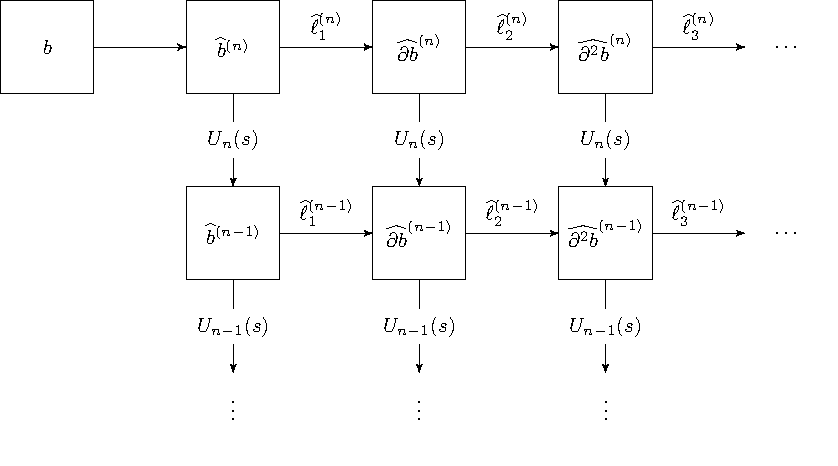
\includegraphics[width=0.875\textwidth]{tikz_filtration.pdf}
  \centering
  \captionsetup{width=.75\linewidth}
  \caption{Filtering errors}
  \label{fig:error-filtration}
\end{figure}

In \texttt{CompDeCasteljau} (Algorithm~\ref{alg:comp-de-casteljau}), after
a single stage of error filtering we
``give up'' and use \(\cdb{1}\) instead of
\(\db{1}\) (without keeping around any information about the
round-off error). In order to obtain results that are as accurate as if
computed in \(K\) times the working precision, we must continue filtering
(see Figure~\ref{fig:error-filtration})
errors down \((K - 1)\) times, and only at the final level do we accept
the rounded
\(\cdb{K - 1}\) in place of the exact
\(\db{K - 1}\).

When computing \(\cdb{F}\) (i.e. the error after
\(F\) stages of filtering)
there will be several sources of round-off. In particular, there will be
\begin{itemize}
\item errors when computing \(\widehat{\ell}_{F, j}^{(k)}\) from the
  terms in \(\ell_{F, j}^{(k)}\)
\item an error
for the ``missing'' \(\rho \cdot \cdb{F}_j^{(k + 1)}\) in
\((1 - s) \cdot \cdb{F}_j^{(k + 1)}\)
\item an error from the product
  \(\widehat{r} \otimes \cdb{F}_j^{(k + 1)}\)
\item an error from the product
  \(s \otimes \cdb{F}_{j + 1}^{(k + 1)}\)
\item two errors from the two \(\oplus\) when combining the three
  terms in
  \(\widehat{\ell}_{F, j}^{(k)} \oplus
  \left(s \otimes \cdb{F}_{j + 1}^{(k + 1)}\right) \oplus
  \left(\widehat{r} \otimes \cdb{F}_j^{(k + 1)}\right)\)
\end{itemize}
For example, in~\eqref{ell-j}:
%% H/T: https://tex.stackexchange.com/a/154333/32270
\begin{equation}
\ell_{1, j}^{(k)} =
    \underbrace{\vphantom{\rho \cdot \widehat{b}_j^{(k + 1)}} \pi_1}_{
        \vphantom{(1 - s) \widehat{b}_j^{(k + 1)}}
        P_1 = \widehat{r} \otimes \widehat{b}_j^{(k + 1)}} +
    \underbrace{\vphantom{\rho \cdot \widehat{b}_j^{(k + 1)}} \pi_2}_{
        \vphantom{(1 - s) \widehat{b}_j^{(k + 1)}}
        P_2 = s \otimes \widehat{b}_{j + 1}^{(k + 1)}} +
    \underbrace{\vphantom{\rho \cdot \widehat{b}_j^{(k + 1)}} \sigma_3}_{
        \vphantom{(1 - s) \widehat{b}_j^{(k + 1)}}
        P_1 \oplus P_2} +
    \underbrace{\rho \cdot \widehat{b}_j^{(k + 1)}}_{
        (1 - s) \widehat{b}_j^{(k + 1)}}
\end{equation}
After each stage, we'll always have
\begin{equation}
\ell_{F, j}^{(k)} = e_1 + \cdots + e_{5F - 2} + \rho \cdot
\cdb{F - 1}_j^{(k + 1)}
\end{equation}
where the terms \(e_1, \ldots, e_{5F - 2}\) come from using \texttt{TwoSum}
and \texttt{TwoProd} when computing \(\cdb{F - 1}_j^{(k)}\)
and the \(\rho\) term comes from the round-off
in \(1 \ominus s\) when multiplying \((1 - s)\) by
\(\cdb{F - 1}_j^{(k + 1)}\). With this in mind, we
can define an EFT (\texttt{LocalErrorEFT}) that computes
\(\widehat{\ell}\) and tracks all round-off errors generated in
the process:

\begin{breakablealgorithm}
  \caption{\textit{EFT for computing the local error.}}
  \label{alg:local-error-eft}

  \begin{algorithmic}
    \Function{\(\left[\eta, \widehat{\ell}\right] =
        \mathtt{LocalErrorEFT}\)}{$e, \rho, \delta b$}
      \State \(L = \texttt{length}(e)\)
      \\
      \State \(\left[\widehat{\ell}, \eta_1\right] =
          \mathtt{TwoSum}(e_1, e_2)\)
      \For{\(j = 3, \ldots, L\)}
        \State \(\left[\widehat{\ell}, \eta_{j - 1}\right] =
            \mathtt{TwoSum}\left(\widehat{\ell}, e_j\right)\)
      \EndFor
      \\
      \State \(\left[P, \eta_L\right] =
          \mathtt{TwoProd}\left(\rho, \delta b\right)\)
      \State \(\left[\widehat{\ell}, \eta_{L + 1}\right] =
          \mathtt{TwoSum}\left(\widehat{\ell}, P\right)\)
    \EndFunction
  \end{algorithmic}
\end{breakablealgorithm}

\noindent With this EFT in place\footnote{And the related
\texttt{LocalError} in Algorithm~\ref{alg:local-error}}, we can
perform \((K - 1)\) error filtrations. Once we've computed the \(K\) stages
of global errors, they can be combined with
\texttt{SumK} (Algorithm~\ref{alg:sum-k}) to produce a sum that is as
accurate as if computed in \(K\) times the working precision.

\begin{breakablealgorithm}
  \caption{\(K\)-\textit{compensated de Casteljau algorithm.}}
  \label{alg:k-comp-de-casteljau}

  \begin{algorithmic}
    \Function{\(\mathtt{result} = \mathtt{CompDeCasteljauK}\)}{$b, s, K$}
      \State \(n = \texttt{length}(b) - 1\)
      \State \(\left[\widehat{r}, \rho\right] = \mathtt{TwoSum}(1, -s)\)
      \\
      \For{\(j = 0, \ldots, n\)}
        \State \(\widehat{b}_j^{(n)} = b_j\)
        \For{\(F = 1, \ldots, K - 1\)}
          \State \(\cdb{F}_j^{(n)} = 0\)
        \EndFor
      \EndFor
      \\
      \For{\(k = n - 1, \ldots, 0\)}
        \For{\(j = 0, \ldots, k\)}
          \State \(\left[P_1, \pi_1\right] = \mathtt{TwoProd}\left(
              \widehat{r}, \widehat{b}_j^{(k + 1)}\right)\)
          \State \(\left[P_2, \pi_2\right] = \mathtt{TwoProd}\left(
              s, \widehat{b}_{j + 1}^{(k + 1)}\right)\)
          \State \(\left[\widehat{b}_j^{(k)}, \sigma_3\right] =
              \mathtt{TwoSum}(P_1, P_2)\)
          \\
          \State \(e = \left[\pi_1, \pi_2, \sigma_3\right]\)
          \State \(\delta b = \widehat{b}_j^{(k + 1)}\)
          \\
          \For{\(F = 1, \ldots, K - 2\)}
            \State \(\left[\eta, \widehat{\ell}\right] =
                \mathtt{LocalErrorEFT}(e, \rho, \delta b)\)
            \State \(L = \texttt{length}(\eta)\)
            \\
            \State \(\left[P_1, \eta_{L + 1}\right] = \mathtt{TwoProd}\left(
                s, \cdb{F}_{j + 1}^{(k + 1)}\right)\)
            \State \(\left[S_2, \eta_{L + 2}\right] =
                \mathtt{TwoSum}\left(\widehat{\ell}, P_1\right)\)
            \State \(\left[P_3, \eta_{L + 3}\right] = \mathtt{TwoProd}\left(
                \widehat{r}, \cdb{F}_j^{(k + 1)}\right)\)
            \State \(\left[\cdb{F}_j^{(k)}, \eta_{L + 4}\right]
                = \mathtt{TwoSum}\left(S_2, P_3\right)\)
            \\
            \State \(e = \eta\)
            \State \(\delta b = \cdb{F}_j^{(k + 1)}\)
          \EndFor
          \\
          \State \(\widehat{\ell} =
                \mathtt{LocalError}(e, \rho, \delta b)\)
          \State \(\cdb{K - 1}_j^{(k)} =
              \widehat{\ell} \oplus
              \left(s \otimes \cdb{K - 1}_{j + 1}^{(k + 1)}
              \right) \oplus
              \left(\widehat{r} \otimes
              \cdb{K - 1}_j^{(k + 1)}\right)\)
        \EndFor
      \EndFor
      \\
      \State \(\mathtt{result} = \mathtt{SumK}\left(\left[
        \widehat{b}_0^{(0)}, \ldots, \cdb{K - 1}_0^{(0)}\right], K\right)\)
    \EndFunction
  \end{algorithmic}
\end{breakablealgorithm}

\noindent Noting that \(\ell_{F, j}\) contains \(5F - 1\) terms, one can
show that \texttt{CompDeCasteljauK} (Algorithm~\ref{alg:k-comp-de-casteljau})
requires
\begin{equation}
(15K^2 + 11K - 34)T_n + 6K^2 - 11K + 11 =
\bigO{n^2 K^2}
\end{equation}
flops to evaluate a degree \(n\) polynomial, where \(T_n\) is the
\(n\)th triangular number. As a comparison, the non-compensated form of
de Casteljau requires \(3 T_n + 1\) flops. In total this will require
\((3K - 4)T_n\) uses of \texttt{TwoProd}. On hardware that supports
FMA, \texttt{TwoProdFMA} (Algorithm~\ref{alg:two-prod-fma}) can be used
instead, lowering the flop count by \(15(3K - 4)T_n\). Another way
to lower the total flop count is to just use
\(\widehat{b}_0^{(0)} \oplus \cdots \oplus \cdb{K - 1}_0^{(0)}\)
instead of \texttt{SumK}; this will reduce the total by
\(6(K - 1)^2\) flops. When using a standard sum, the results produced
are (empirically) identical to those with \texttt{SumK}. This makes
sense: the whole point of \texttt{SumK}
is to filter errors in a summation so that the final operation produces
a sum of the form \(v_1 \oplus \cdots \oplus v_K\) where each
term is smaller than the previous by a factor of \(\mach\). This
property is already satisfied for the \(\cdb{F}_0^{(0)}\) so in
practice the \(K\)-compensated summation is likely not needed.

\subsection{Error bound for polynomial evaluation}

\begin{theorem}[\cite{Ogita2005}, Proposition 4.10]\label{thm:sum-k}
A summation can be computed (\texttt{SumK}, Algorithm~\ref{alg:sum-k})
with results that are as accurate as if computed in \(K\) times the
working precision. When computed this way, the result satisfies:
\begin{equation}
\left|\mathtt{SumK}(v, K) - \sum_{j = 1}^n v_j\right| \leq
\left(\mach + 3 \gamma_{n - 1}^2\right) \left|\sum_{j = 1}^n v_j\right| +
\gamma_{2n - 2}^K \sum_{j = 1}^n \left|v_j\right|.
\end{equation}
\end{theorem}

\begin{lemma}[\cite{Jiang2010}, Theorem 4]\label{lemma:db-lemma}
The second order error \(\db{2}^{(0)}_0\) satisfies\footnote{The authors
  missed one round-off error so used \(\gamma_{3n + 1}\) where
  \(\gamma_{3n + 2}\) would have followed from their arguments.}
\begin{equation}
  \left|\db{1}^{(0)}_0 - \cdb{1}^{(0)}_0\right| =
  \left|\db{2}^{(0)}_0\right| \leq 2 \gamma_{3n + 2} \gamma_{3(n - 1)}
  \widetilde{p}(s).
\end{equation}
\end{lemma}

To enable a bound on the \(K\) order error \(\db{K}^{(0)}_0\), it's necessary
to understand the difference between the exact local errors \(\ell_{F, j}\)
and the computed equivalents \(\widehat{\ell}_{F, j}\). To do this, we define
\begin{equation}
\widetilde{\ell}_{F, j} \coloneqq \left|e_1\right| +
\cdots + \left|e_{5F - 2}\right| + \left|\rho \cdot
\cdb{F - 1}_j^{(k + 1)}\right|.
\end{equation}

\begin{lemma}\label{lemma:ell-tilde}
The local error bounds \(\widetilde{\ell}_{F, j}\) satisfy:
\begin{align}
\widetilde{\ell}_{1, j}^{(k)} &\leq
  \gamma_3 \left(
  (1 - s) \left|\widehat{b}_j^{(k + 1)}\right| +
  s \left|\widehat{b}_{j + 1}^{(k + 1)}\right|\right)
  \label{ell-tilde-1} \\
\widetilde{\ell}_{F + 1, j}^{(k)} &\leq
  \gamma_3 \left(
  (1 - s) \left|\cdb{F}_j^{(k + 1)}\right| +
  s \left|\cdb{F}_{j + 1}^{(k + 1)}\right|\right) +
  \gamma_{5F} \cdot \widetilde{\ell}_{F, j}^{(k)}
  \text{ for } F \geq 1.
\end{align}
\end{lemma}

As we'll see soon (Lemma~\ref{lemma:k-order}), putting a bound on
sums of the form \(\sum_{j = 0}^k \ell_{F, j}^{(k)} B_{j, k}(s)\) will
be useful to get an overall bound on the relative error for
\texttt{CompDeCasteljauK}, so we define
\(L_{F, k} \coloneqq \sum_{j = 0}^k \ell_{F, j}^{(k)} B_{j, k}(s)\).

\begin{lemma}\label{lemma:L-and-D-bounds}
For \(s \in \left[0, 1\right]\), the Bernstein-type error sum defined above
satisfies the following bounds:
\begin{align}
L_{F, n - k} &\leq \left[\left(3^F \binom{k}{F - 1} + \bigO{k^{F - 1}}\right)
  \mach^F + \bigO{\mach^{F + 1}}\right] \cdot \widetilde{p}(s) \\
\sum_{k = 0}^{n - 1} \gamma_{3k + 5F} L_{F, k} &\leq
  \left[\left(3^{F + 1} \binom{n}{F + 1} + \bigO{n^F}\right)
  \mach^{F + 1} + \bigO{\mach^{F + 2}}\right] \cdot \widetilde{p}(s).
  \label{L-sum-bound}
\end{align}
In particular, this means that
\(\sum_{k = 0}^{n - 1} \gamma_{3k + 5F} L_{F, k} =
\bigO{(3 n \mach)^{F + 1}} \cdot \widetilde{p}(s)\).
\end{lemma}

See Appendix~\ref{chap:appendix-proof-details} for details on
proving Lemma~\ref{lemma:ell-tilde} and Lemma~\ref{lemma:L-and-D-bounds}.

\begin{lemma}\label{lemma:k-order}
The \(K\) order error \(\db{K}^{(0)}_0\) satisfies
\begin{equation}
  \left|\db{K - 1}^{(0)}_0 - \cdb{K - 1}^{(0)}_0\right| =
  \left|\db{K}^{(0)}_0\right| \leq
  \left[\left(3^{K} \binom{n}{K} + \bigO{n^{K - 1}}\right)
  \mach^{K} + \bigO{\mach^{K + 1}}\right] \cdot \widetilde{p}(s).
\end{equation}
\end{lemma}

\begin{proof}
As in \eqref{matrix-de-casteljau}, we can express the compensated
de Casteljau algorithm as
\begin{equation}
\db{F}^{(k)} = U_{k + 1} \db{F}^{(k + 1)} + \ell_{F}^{(k)}
\Longrightarrow \db{F}^{(0)} = \sum_{k = 0}^{n - 1}
U_1 \cdots U_k \ell_F^{(k)} = \sum_{k = 0}^{n - 1}
\left[\sum_{j = 0}^k \ell_{F, j}^{(k)} B_{j, k}(s)\right].
\end{equation}
For the inexact equivalent of these things, first note that
\(\widehat{r} = (1 - s)(1 + \delta)\). Due to this,
we put the \(\widehat{r}\) term at the end of each update step to reduce
the amount of round-off:
\begin{align}
  \cdb{F}_j^{(k)} &=
  \widehat{\ell}_{F, j}^{(k)} \oplus
  \left(s \otimes \cdb{F}_{j + 1}^{(k + 1)}\right) \oplus
  \left(\widehat{r} \otimes \cdb{F}_j^{(k + 1)}\right) \\
&= (1 - s) \cdot \cdb{F}_j^{(k + 1)}(1 + \theta_3) +
  s \cdot \cdb{F}_{j + 1}^{(k + 1)}(1 + \theta_3) +
  \widehat{\ell}_{F, j}^{(k)} (1 + \theta_2) \\
\Longrightarrow \cdb{F}^{(k)} &=
  U_{k + 1} \cdb{F}^{(k + 1)}(1 + \theta_3) +
  \widehat{\ell}_{F}^{(k)} (1 + \theta_2) \\
\Longrightarrow \cdb{F}^{(0)} &=
  \sum_{k = 0}^{n - 1}
  U_1 \cdots U_k \widehat{\ell}_F^{(k)} (1 + \theta_{3k + 2})
  = \sum_{k = 0}^{n - 1}
  \left[\sum_{j = 0}^k \widehat{\ell}_{F, j}^{(k)} (1 + \theta_{3k + 2})
    B_{j, k}(s)\right].
\end{align}
Since
\begin{equation}
\db{F + 1}_0^{(0)} = \db{F}_0^{(0)} - \cdb{F}_0^{(0)} = \sum_{k = 0}^{n - 1}
\sum_{j = 0}^k \left(\ell_{F, j}^{(k)} -
\widehat{\ell}_{F, j}^{(k)} (1 + \theta_{3k + 2})\right) B_{j, k}(s)
\end{equation}
it's useful to put a bound on \(\ell_{F, j}^{(k)} -
\widehat{\ell}_{F, j}^{(k)} (1 + \theta_{3k + 2})\). Via
\begin{align}
\widehat{\ell}_{F, j}^{(k)} &= e_1 \oplus \cdots \oplus e_{5F - 2} \oplus
\left(\rho \otimes \cdb{F - 1}_j^{(k + 1)}\right) \\
&= e_1\left(1 + \theta_{5F - 2}\right) + \cdots +
e_{5F - 2}\left(1 + \theta_2\right) +
\rho \cdot \cdb{F - 1}_j^{(k + 1)} \left(1 + \theta_2\right)
\end{align}
we see that
\begin{equation}
\left|\ell_{F, j}^{(k)} -
\widehat{\ell}_{F, j}^{(k)} (1 + \theta_{3k + 2})\right| \leq
\gamma_{3k + 5F} \cdot \widetilde{\ell}_{F, j}^{(k)}
\Longrightarrow
\left|\db{F + 1}_0^{(0)}\right| \leq \sum_{k = 0}^{n - 1}
\gamma_{3k + 5F} \sum_{j = 0}^k \widetilde{\ell}_{F, j}^{(k)} B_{j, k}(s).
\end{equation}
Applying \eqref{L-sum-bound} directly gives
\begin{equation}
\left|\db{F + 1}_0^{(0)}\right| \leq
  \left[\left(3^{F + 1} \binom{n}{F + 1} + \bigO{n^F}\right)
  \mach^{F + 1} + \bigO{\mach^{F + 2}}\right] \cdot \widetilde{p}(s).
\end{equation}
Letting \(K = F + 1\) we have our result.
\end{proof}

\begin{theorem}
If no underflow occurs, \(n \geq 2\) and \(s \in \left[0, 1\right]\)
\begin{multline}
  \frac{\left|p(s) - \mathtt{CompDeCasteljau}(p, s, K)\right|}{
    \left|p(s)\right|} \leq \left[\mach + \bigO{\mach^2}
    \right] + \\
    \left[\left(3^{K} \binom{n}{K} + \bigO{n^{K - 1}}\right) \mach^K +
    \bigO{\mach^{K + 1}}\right] \cond{p, s}.
\end{multline}
\end{theorem}

\begin{proof}
Since
\begin{equation}
\mathtt{CompDeCasteljau}(p, s, K) = \mathtt{SumK}\left(\left[
  \widehat{b}_0^{(0)}, \ldots, \cdb{K - 1}_0^{(0)}\right], K\right),
\end{equation}
applying Theorem~\ref{thm:sum-k} tells us that
\begin{equation}\label{sum-k-applied}
\left|\mathtt{CompDeCasteljau}(p, s, K) - \sum_{F = 0}^{K - 1}
\cdb{F}_0^{(0)}\right| \leq
\left(\mach + 3 \gamma_{n - 1}^2\right) \left|\sum_{F = 0}^{K - 1}
\cdb{F}_0^{(0)}\right| +
\gamma_{2n - 2}^K \sum_{F = 0}^{K - 1} \left|\cdb{F}_0^{(0)}\right|.
\end{equation}
Since
\begin{equation}
p(s) = b_0^{(0)} = \widehat{b}_0^{(0)} + \db{1}_0^{(0)}
= \cdots
= \widehat{b}_0^{(0)} + \cdb{1}_0^{(0)} + \cdots
+ \cdb{K - 1}_0^{(0)} + \db{K}_0^{(0)}
\end{equation}
we have
\begin{gather}
\left|\sum_{F = 0}^{K - 1} \cdb{F}_0^{(0)}\right|
\leq \left|p(s)\right| + \left|\db{K}_0^{(0)}\right| \quad \text{and} \\
\left|\mathtt{CompDeCasteljau}(p, s, K) - p(s)\right| \leq
\left|\mathtt{CompDeCasteljau}(p, s, K) - \sum_{F = 0}^{K - 1}
\cdb{F}_0^{(0)}\right| +
\left|\db{K}_0^{(0)}\right| \label{triangle-ps}.
\end{gather}
Due to Lemma~\ref{lemma:k-order}, \(\db{F}_0^{(0)} =
\bigO{\mach^F} \widetilde{p}(s)\), hence
\begin{align}
\left(\mach + 3 \gamma_{n - 1}^2\right) \left|\sum_{F = 0}^{K - 1}
\cdb{F}_0^{(0)}\right| &\leq
\left[\mach + \bigO{\mach^2}\right] \left|p(s)\right| +
\bigO{\mach^{K + 1}} \widetilde{p}(s) \\
\gamma_{2n - 2}^K \sum_{F = 0}^{K - 1} \left|\cdb{F}_0^{(0)}\right| &\leq
\gamma_{2n - 2}^K \left|\widehat{b}_0^{(0)}\right| +
\bigO{\mach^{K + 1}} \widetilde{p}(s) \\
&\leq
\gamma_{2n - 2}^K \left[\left|p(s)\right| +
  \bigO{\mach} \widetilde{p}(s)\right] +
\bigO{\mach^{K + 1}} \widetilde{p}(s).
\end{align}
Combining this with \eqref{sum-k-applied} and \eqref{triangle-ps}, we
see
\begin{align}
& \left|\mathtt{CompDeCasteljau}(p, s, K) - p(s)\right| \\
\leq &
\left[\mach + \bigO{\mach^2}\right] \left|p(s)\right| +
\left|\db{K}_0^{(0)}\right| +
\bigO{\mach^{K + 1}} \widetilde{p}(s) \\
\leq &
\left[\mach + \bigO{\mach^2}\right] \left|p(s)\right| +
\left[\left(3^{K} \binom{n}{K} + \bigO{n^{K - 1}}\right) \mach^K +
\bigO{\mach^{K + 1}} \right]
\widetilde{p}(s).
\end{align}
Dividing this by \(\left|p(s)\right|\), we have our result.
\end{proof}

For the first few values of \(K\) the coefficient of
\(\cond{p, s}\) in the bound is
\begin{center}
  \begin{tabular}{>{$}c<{$} c >{$}c<{$}}
    K & Method & \text{Multiplier} \\
    \midrule
    1 & \texttt{DeCasteljau} & 3 \binom{n}{1} \mach =
      3n \mach \approx \gamma_{3n} \\[0.125cm]
    2 & \texttt{CompDeCasteljau} & \left[9 \binom{n}{2} +
      15 \binom{n}{1}\right]\mach^2 = \frac{3n(3n + 7)}{2} \mach^2
      \approx \frac{1}{4} \cdot 2 \gamma_{3n}^2 \\[0.125cm]
    3 & \texttt{CompDeCasteljau3} & \left[27 \binom{n}{3} +
      135 \binom{n}{2} + 150 \binom{n}{1}\right] \mach^3 =
      \frac{3n(3n^2 + 36n + 61)}{2} \mach^3 \\[0.125cm]
    4 & \texttt{CompDeCasteljau4} & \left[81 \binom{n}{4} + 810 \binom{n}{3} +
      2475 \binom{n}{2} + 2250 \binom{n}{1}\right] \mach^4 \\[0.125cm]
  \end{tabular}
\end{center}
See the \hyperref[proof:L-and-D-bounds]{proof} of
Lemma~\ref{lemma:L-and-D-bounds} for more details on where these
polynomials come from.

\section{Numerical experiments}\label{sec:numerical}

\begin{figure}
  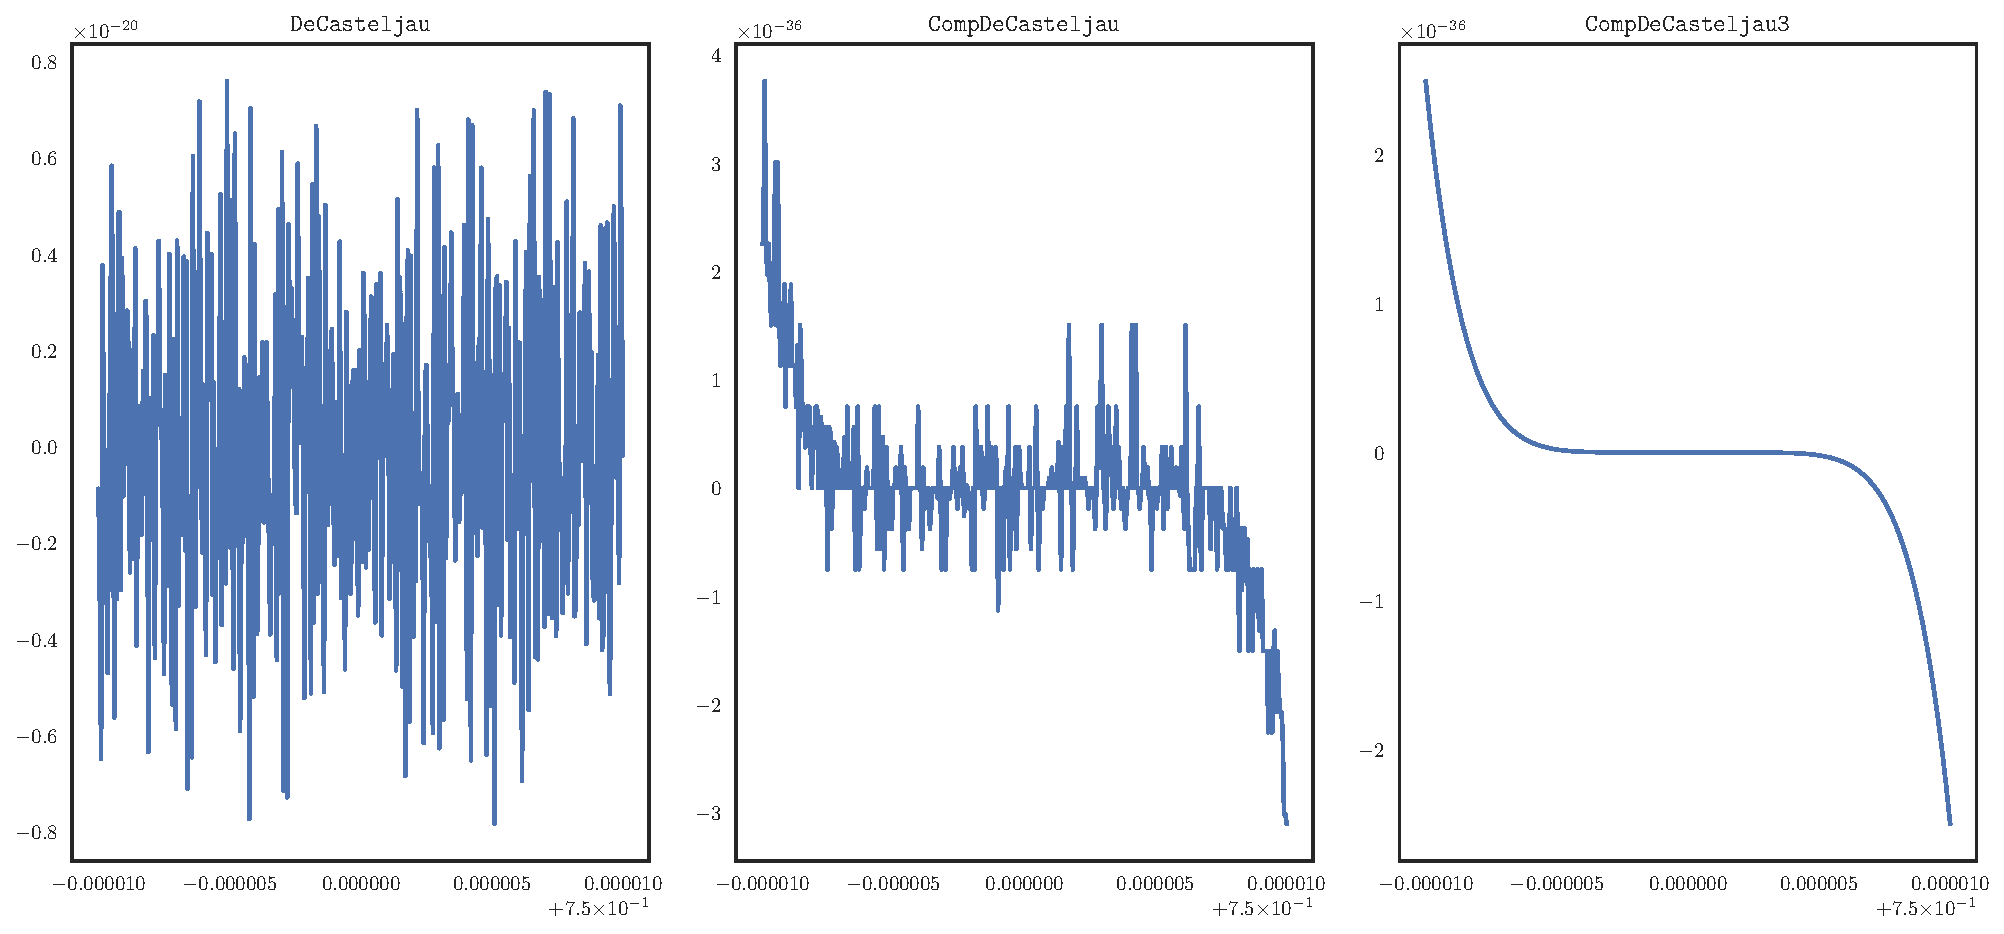
\includegraphics[width=0.9375\textwidth]{../images/k-compensated/de_casteljau_smooth_drawing.pdf}
  \centering
  \captionsetup{width=.75\linewidth}
  \caption{Evaluation of \(p(s) = (s - 1)\left(s - 3/4\right)^7\)
    in the neighborhood of its multiple root \(3/4\).}
  \label{fig:smooth-drawing}
\end{figure}

All experiments were performed in IEEE-754 double precision.
As in \cite{Jiang2010}, we consider the evaluation in the neighborhood
of the multiple root of \(p(s) = (s - 1)\left(s - 3/4\right)^7\),
written in Bernstein form.
Figure~\ref{fig:smooth-drawing} shows the evaluation of \(p(s)\) at
the 401 equally spaced\footnote{It's worth noting that \(0.1\) cannot
be represented exactly in IEEE-754 double precision (or any binary
arithmetic for that matter). Hence (most of) the points of the form
\(a + b \cdot 10^{-c}\) can only be approximately represented.} points
\(\left\{\frac{3}{4} + j \frac{10^{-7}}{2}\right\}_{j=-200}^{200}\)
with \texttt{DeCasteljau} (Algorithm~\ref{alg:de-casteljau}),
\texttt{CompDeCasteljau} (Algorithm~\ref{alg:comp-de-casteljau})
and \texttt{CompDeCasteljau3} (Algorithm~\ref{alg:k-comp-de-casteljau}
with \(K = 3\)). We see that \texttt{DeCasteljau} fails to get the
magnitude correct, \texttt{CompDeCasteljau} has the right shape but
lots of noise and \texttt{CompDeCasteljau3} is able to smoothly evaluate
the function. This is in contrast to a similar figure in \cite{Jiang2010},
where the plot was smooth for the 400 equally spaced points
\(\left\{\frac{3}{4} + \frac{10^{-4}}{2} \frac{2j - 399}{399}
\right\}_{j=0}^{399}\). The primary difference is that as the interval
shrinks by a factor of \(\approx \frac{10^{-4}}{10^{-7}} = 10^3\), the
condition number goes up by \(\approx 10^{21}\) and \texttt{CompDeCasteljau}
is no longer accurate.

\begin{figure}
  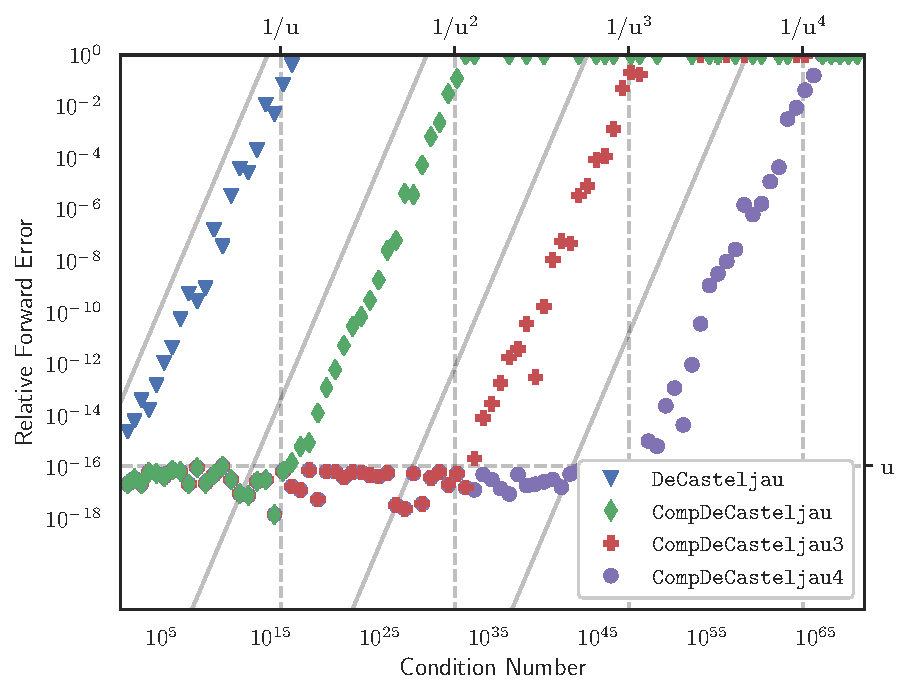
\includegraphics[width=0.8125\textwidth]{../images/k-compensated/de_casteljau_rel_error.pdf}
  \centering
  \captionsetup{width=.75\linewidth}
  \caption{Accuracy of evaluation of \(p(s) = (s - 1)\left(s - 3/4\right)^7\)
    represented in Bernstein form.}
  \label{fig:compensated-k}
\end{figure}

Figure~\ref{fig:compensated-k} shows the relative forward errors compared
against the condition number. To compute relative errors, each input and
coefficient is converted to a fraction (i.e. infinite precision) and
\(p(s)\) is computed exactly as a fraction, then
compared to the corresponding computed values. Similar tools are used to
\textbf{exactly} compute the condition number, though here we can rely
on the fact that \(\widetilde{p}(s) = (s - 1)
\left(s/2 - 3/4\right)^7\). Once the relative errors and
condition numbers are computed as fractions, they are rounded to the
nearest IEEE-754 double precision value. As in \cite{Jiang2010}, we use
values \(\left\{\frac{3}{4} - (1.3)^j\right\}_{j=-5}^{-90}\)\footnote{As with
\(0.1\), it's worth noting that \((1.3)^j\) can't be represented exactly in
IEEE-754 double precision. However, this geometric series still serves a
useful purpose since it continues to raise \(\cond{p, s}\) as \(j\) decreases
away from \(0\) and because it results in ``random'' changes in the bits of
\(0.75\) that are impacted by subtracting \((1.3)^j\).}. The curves for
\texttt{DeCasteljau} and \texttt{CompDeCasteljau} trace the same paths seen
in \cite{Jiang2010}. In particular, \texttt{CompDeCasteljau} has a relative
error that is \(\bigO{\mach}\) until \(\cond{p, s}\) reaches
\(1 / \mach\), at which point the relative error increases linearly with
the condition number until it becomes \(\bigO{1}\) when
\(\cond{p, s}\) reaches \(1 / \mach^2\).
Similarly, the relative error in \texttt{CompDeCasteljau3}
(Algorithm~\ref{alg:k-comp-de-casteljau} with \(K = 3\))
is \(\bigO{\mach}\) until \(\cond{p, s}\) reaches
\(1 / \mach^2\) at which point the relative error increases linearly
to \(\bigO{1}\) when \(\cond{p, s}\) reaches \(1 / \mach^3\)
and the relative error in \texttt{CompDeCasteljau4}
(Algorithm~\ref{alg:k-comp-de-casteljau} with \(K = 4\))
is \(\bigO{\mach}\) until \(\cond{p, s}\) reaches
\(1 / \mach^3\) at which point the relative error increases linearly
to \(\bigO{1}\) when \(\cond{p, s}\) reaches \(1 / \mach^4\).

\chapter{Accurate Newton's Method for B\'{e}zier Curve Intersection}
\label{chap:compensated-newton}

\section{Introduction}

When using Newton's method to find the root of a function via
\begin{equation}
G\left(\bm{x}\right) = \bm{x} - J^{-1} F\left(\bm{x}\right)
\end{equation}
there are three computations performed that can introduce instability:
evaluation of the residual function \(F\left(\bm{x}\right)\), evaluation
of the Jacobian \(J\) and solution of the linear system \(J \bm{y} =
F\left(\bm{x}\right)\). In \cite{Tisseur2001}, the author showed that by
just using a more precise evaluation of the residual function, the
accuracy of Newton's method can be improved.

This chapter considers Newton's method applied to two problems:
root-finding for polynomials expressed in Bernstein form and
intersection of two B\'{e}zier curves in \(\reals^2\). In both problems,
the compensated de Casteljau method (see Chapter~\ref{chap:k-compensated}) is
used for evaluation of the residual. When evaluating a polynomial
\(p(s)\) this is straightforward, but when evaluating the difference
\(b_1(s) - b_2(t)\) between two curves special care must be taken.

\begin{figure}
  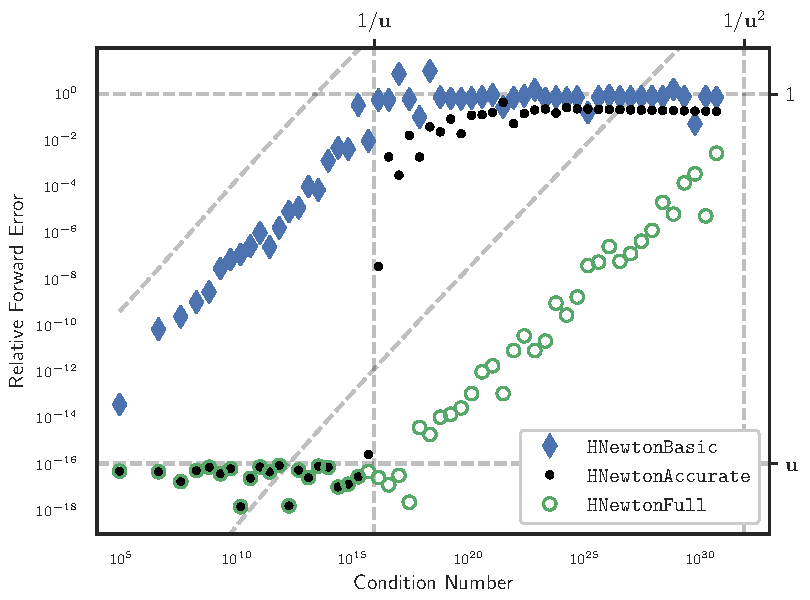
\includegraphics{../images/compensated-newton/newton_jghplus13.pdf}
  \centering
  \captionsetup{width=.75\linewidth}
  \caption{Comparing relative error to condition number when using Newton's
    method to find a root of \(p(s) = (s - 1)^n - 2^{-31}\), where polynomial
    evaluation occurs via Horner's method.}
  \label{fig:jgh+13}
\end{figure}

In \cite{Graillat2008}, the problem of finding simple roots \(\alpha\) of
polynomials \(p(s)\) expressed in the monomial basis is considered.
A standard Newton's method (\texttt{HNewtonBasic}) that evaluates \(p(s)\)
and \(p'(s)\) using Horner's method is compared to a modified Newton's method
(\texttt{HNewtonAccurate}) that evaluates \(p(s)\) with a compensated
Horner's method. This proceeds as in \cite{Tisseur2001}: the evaluation of
the residual is done with greater accuracy but the rest of the process
is the same. When computing a root \(\alpha\), the standard Newton's method
has a relative error that grows linearly with the condition number of the
root (which will be defined in Section~\ref{sec:conditioning}). The
modified Newton's method is fully accurate to machine precision (i.e.
the relative error is \(\bigO{\mach}\)) until \(\cond{\alpha}\) reaches
\(1/\mach\), as seen in Figure~\ref{fig:jgh+13}.

After the point where \texttt{HNewtonAccurate} loses accuracy, we'd
expect a linear increase in relative error based on a compensated
rule of thumb:
\begin{equation}
\frac{\left|\widehat{\alpha} - \alpha\right|}{\left|\alpha\right|} \leq
  c_1 \mach + c_2 \cond{\alpha} \mach^2
\end{equation}
where \(c_1 \mach\) corresponds to rounding into the given
precision and \(c_2 \cond{\alpha} \mach^2\) reflects the
typical error but from computations done with working precision
\(\overline{\mach} = \mach^2\). The point
where the condition number exceeds \(1/\mach\) should correspond to
the point where the second term is larger that the
first term. However, this is not possible unless the
Jacobian (i.e. \(p'(s)\)) is also evaluated with a compensated
method. A second modified Newton's method (\texttt{HNewtonFull}) is
introduced in \cite[Section~8]{Jiang2013} and the author shows that
this second modified Newton's method does indeed follow a compensated
rule of thumb under appropriate conditions. We see in
Figure~\ref{fig:jgh+13} that \texttt{HNewtonFull} enables
\(\bigO{\mach}\) relative errors until the condition number reaches
\(1/\mach\) and then a linear increase in error as the condition number
grows from \(1/\mach\) to \(1/\mach^2\).

We'll proceed similarly for polynomials in
Bernstein form. Since this is a one dimensional Newton's method, improving
the evaluation of the Jacobian is straightforward. The results agree with
what has been observed when using Horner's method for evaluation.

Computing the intersection(s) of two parametric plane curves is a
common task in computational geometry and has many uses, e.g. in
finite element methods that use overlapping curved meshes. Many
methods have been described in the literature to solve this problem.
Algebraic methods such as implicitization and eigenvalue-based
methods (e.g. \cite{Manocha:CSD-92-698}) suffer
from accuracy issues for moderately high degrees and can often be
very complex to implement. Some (\cite{Bates2008}) even rely on symbolic
algebraic manipulations, which can be quite costly since it requires
arbitrary precision.
Geometric methods (e.g. \cite{Sederberg1986, Sederberg1990, Kim1998})
typically use a form of domain splitting to focus on subproblems and
eliminate parts of the domain where an intersection is guaranteed not
to occur. After a domain has been sufficiently reduced, Newton's method
is used for the last few bits of accuracy.

We'll focus on transversal curve intersections that are ill-conditioned.
Transversal intersections are an extension of the concept of a
simple root. A non-transversal intersection occurs when the curves
or tangent at the point of intersection or when one of the curves
has a zero tangent vector at that point, either due to an improper
parameterization (e.g. \(x(s) = s^2, y(s) = s^2 + 1\)) or a cusp.
In many cases, transversal intersections that are ``almost tangent'' have
very high condition numbers.

The chapter is organized as follows. In Section~\ref{sec:conditioning}
we define and discuss the conditioning of both a simple root and
a transversal intersection. In Section~\ref{sec:compensated-simple-roots}
we describe two compensated Newton's methods for finding simple roots
and perform a numerical experiment verifying the expected behavior.
In Section~\ref{sec:compensated-curve-intersect} we describe a
compensated Newton's method for B\'{e}zier curve intersection and
perform sever numerical experiements to verify the expected behavior
on both transversal intersections and tangent intersections (i.e.
intersections with infinite condition number).
Section~\ref{sec:false-starts} acts as a
coda: it describes some failed attempts at constructing numerical
examples. This section provides an in-depth discussion of a particular
family of polynomials that has much better than expected conditioning
when written in the Bernstein basis.

\section{Problem conditioning}\label{sec:conditioning}

Consider a smooth function \(F: \reals^n \longrightarrow \reals^n\)
with Jacobian \(F_{\bm{x}} = J\). We want to consider a special class of
functions of the form \(F\left(\bm{x}\right) = \sum_j c_j
\phi_j\left(\bm{x}\right)\) where the basis
functions \(\phi_j\) are also smooth functions on \(\reals^n\)
and each \(c_j \in \reals\). We want to consider the effects on a root
\(\bm{\alpha} \in \reals^n\) of a perturbation in one of the
coefficients \(c_j\). We examine the perturbed functions
\begin{equation}
G(x, \delta) = F\left(\bm{x}\right) + \delta \phi_j\left(\bm{x}\right).
\end{equation}
Since \(G\left(\bm{\alpha}, 0\right) = \bm{0}\), if \(J^{-1}\) exists at
\(\bm{x} = \bm{\alpha}\) then
the implicit function theorem tells us that we can define
\(\bm{x}\) via
\begin{equation}
G\left(\bm{x}\left(\delta\right), \delta\right) = \bm{0}.
\end{equation}
Taking the derivative with respect to \(\delta\) we find that
\(\bm{0} = G_{\bm{x}} \bm{x}_{\delta} + G_{\delta}\). Plugging in
\(\delta = 0\) we find that \(0 = J\left(\bm{\alpha}\right) \bm{x}_{\delta} +
\phi_j\left(\bm{\alpha}\right)\), hence we
conclude that
\begin{equation}
\bm{x}\left(\delta\right) = \bm{\alpha} - J\left(\bm{\alpha}\right)^{-1}
  \phi_j\left(\bm{\alpha}\right) \delta + \bigO{\delta^2}.
\end{equation}
This gives a relative condition number (for the root) of
\begin{equation}
\frac{\left \lVert J\left(\bm{\alpha}\right)^{-1}
  \phi_j\left(\bm{\alpha}\right) \right \rVert}{
  \left \lVert \bm{\alpha} \right \rVert}.
\end{equation}

By considering perturbations in \textbf{all} of the coefficients:
\(\left|\delta_j\right| \leq \eps \left|c_j\right|\), a similar analysis
gives a root function
\begin{equation}
\bm{x}\left(\delta_0, \ldots, \delta_n\right) = \bm{\alpha} -
  J\left(\bm{\alpha}\right)^{-1} \sum_{j = 0}^n \delta_j
  \phi_j\left(\bm{\alpha}\right) + \bigO{\eps^2}.
\end{equation}
With this, we can define a root condition number
\begin{equation}\label{eq:abstract-cond-num}
\kappa_{\bm{\alpha}} =
  \lim_{\eps \to 0} \left(\sup \frac{\left \lVert\delta \bm{\alpha}
  \right \rVert / \eps}{\left \lVert\bm{\alpha}\right \rVert}\right) =
  \lim_{\eps \to 0} \left(\sup \frac{\left \lVert
  J\left(\bm{\alpha}\right)^{-1} \sum_j \delta_j
  \phi_j\left(\bm{\alpha}\right) \right \rVert / \eps}{
  \left \lVert\bm{\alpha}\right \rVert}\right).
\end{equation}

When \(n = 1\), \(J^{-1}\) is simply \(1 / F'\) and we find
\begin{equation}
\kappa_{\alpha} =
  \frac{1}{\left|\alpha F'(\alpha)\right|} \sum_{j = 0}^n \left|
  c_j \phi_j(\alpha)\right|.
\end{equation}
This value is given by the triangle inequality applied to
\(\delta \alpha\)  and equality can be attained since the sign
of each \(\delta_j = \pm c_j \eps\) can be modified at will to make
\(\phi_j(\alpha) \delta_j = \left|\phi_j(\alpha) c_j\right| \eps\).

When \(n > 1\), the triangle inequality tells us that
\begin{equation}
\kappa_{\bm{\alpha}} =
  \lim_{\eps \to 0} \left(\sup \frac{\left \lVert\delta \bm{\alpha} /
  \eps\right \rVert}{\left \lVert\bm{\alpha}\right \rVert}\right) \leq
  \frac{1}{\left \lVert\bm{\alpha}\right \rVert} \sum_{j = 0}^n
  \left|c_j\right| \left \lVert J\left(\bm{\alpha}\right)^{-1}
  \phi_j(\bm{\alpha})\right \rVert.
\end{equation}
However, this bound is only attainable if all
\(\phi_j(\bm{\alpha})\) are parallel. However, we'll seldom need to
compute the exact condition number and are instead typically
interested in the order of magnitude. In this case a lower
bound
\begin{equation}
\frac{1}{\left \lVert\bm{\alpha}\right \rVert}
\max_j \left|c_j\right| \left \lVert J\left(\bm{\alpha}\right)^{-1}
\phi_j(\bm{\alpha})\right \rVert
\end{equation}
for \(\kappa_{\bm{\alpha}}\)
will suffice as an approximate condition number.

For an example, consider
\begin{equation}
\phi_0 = \left[ \begin{array}{c} x_0 \\ 2 \\ 0 \end{array}\right],
\phi_1 = \left[ \begin{array}{c} 0 \\ x_1 \\ 3 \end{array}\right],
\phi_2 = \left[ \begin{array}{c} 2 \\ 0 \\ x_2 \end{array}\right],
F = \phi_0 + 2 \phi_1 + 3 \phi_2,
\bm{\alpha} = \left[ \begin{array}{c} -6 \\ -1 \\ -2 \end{array}\right].
\end{equation}
For a given \(\eps\), the maximum root perturbation occurs when
\(\delta_0 = \eps, \delta_1 = 2 \eps, \delta_2 = -3 \eps\) and
gives
\(\left \lVert J\left(\bm{\alpha}\right)^{-1} \sum_j
\delta_j \phi_j\left(\bm{\alpha}\right) \right \rVert
= 4 \sqrt{10} \eps \approx 12.65 \eps\).
The pessimistic triangle inequality bound gives
\(\sum_j \left|c_j\right| \left \lVert J\left(\bm{\alpha}\right)^{-1}
\phi_j(\bm{\alpha})\right \rVert \approx 14.64 \eps\) and the
maximum individual perturbation is \(2 \sqrt{10} \eps \approx 6.325 \eps\)
(this occurs when \(\delta_0 = \delta_1 = 0, \delta_2 = \pm 3 \eps\)).

In this general framework, we can define a condition number both
for a simple root of a polynomial in Bernstein form and for the
intersection of two planar B\'{e}zier curves. For the first,
\(\phi_j(s) = \binom{n}{j} (1 - s)^{n - j} s^j\) the Bernstein basis
functions, a polynomial \(p(s) = \sum_j b_j \phi_j(s)\) with
a simple root \(\alpha \in \left(0, 1\right]\) has root condition number
\begin{equation}
\kappa_{\alpha} =
  \frac{1}{\alpha \left|p'(\alpha)\right|} \sum_{j = 0}^n \left|
  b_j \phi_j(\alpha)\right| = \frac{\widetilde{p}(\alpha)}{
  \alpha \left|p'(\alpha)\right|}.
\end{equation}
For the intersection of a degree \(m\) curve \(b_1(s)\) and
a degree \(n\) curve \(b_2(t)\), we have basis functions
\begin{multline}
\phi_{0, -1, 1} = \left[ \begin{array}{c} B_{0, m}(s) \\ 0 \end{array}\right],
\phi_{0, -1, 2} = \left[ \begin{array}{c} 0 \\ B_{0, m}(s) \end{array}\right],
\cdots, \\
\phi_{m, -1, 1} = \left[ \begin{array}{c} B_{m, m}(s) \\ 0 \end{array}\right],
\phi_{m, -1, 2} = \left[ \begin{array}{c} 0 \\
  B_{m, m}(s) \end{array}\right], \\
\phi_{-1, 0, 1} = \left[ \begin{array}{c} -B_{0, n}(t) \\
  0 \end{array}\right],
\phi_{-1, 0, 2} = \left[ \begin{array}{c} 0 \\
  -B_{0, n}(t) \end{array}\right], \cdots, \\
\phi_{-1, n, 1} = \left[ \begin{array}{c} -B_{n, n}(t) \\
  0 \end{array}\right], \phi_{-1, n, 2} = \left[ \begin{array}{c} 0 \\
  -B_{n, n}(t) \end{array}\right].
\end{multline}
Since \(F(s, t) = b_1(s) - b_2(t)\) we have Jacobian \(J(s, t) =
\left[ \begin{array}{c c} b_1'(s) & -b_2'(t) \end{array}\right]\). We'll
consider a transversal intersection \(F(\alpha, \beta) = \bm{0}\) with
\(\det J(\alpha, \beta) \neq 0\). Since each of the
\(\phi_j\) is just a scalar multiple of the standard basis
vectors, writing \(J^{-1} = \left[ \begin{array}{c c}
\bm{v}_1 & \bm{v}_2 \end{array}\right]\), we have
\begin{multline}
J\left(\alpha, \beta\right)^{-1} \sum_{\bm{j}} \delta_{\bm{j}}
  \phi_{\bm{j}}\left(\alpha, \beta\right) = \left[\sum_{i = 0}^m
  \delta_{i, -1, 1} B_{i, m}\left(\alpha\right) + \sum_{j = 0}^n
  \delta_{-1, j, 1} B_{j, n}\left(\beta\right)\right] \bm{v}_1 \\
+ \left[\sum_{i = 0}^m
  \delta_{i, -1, 2} B_{i, m}\left(\alpha\right) + \sum_{j = 0}^n
  \delta_{-1, j, 2} B_{j, n}\left(\beta\right)\right] \bm{v}_2 =
  \nu_1 \bm{v}_1 + \nu_2 \bm{v}_2.
\end{multline}
where
\begin{equation}\label{eq:nu-bounds}
\left|\nu_k\right| / \eps \leq \sum_{i = 0}^m
  \left|c_{i, -1, k}\right| B_{i, m}\left(\alpha\right) + \sum_{j = 0}^n
  \left|c_{-1, j, k}\right| B_{j, n}\left(\beta\right) = \mu_k
\end{equation}
and the bound can be attained for both \(k = 1, 2\) by making the
signs of the \(\delta_{\bm{j}}\) agree. If we name the components of each
curve via
\(b_1(s) = \left[ \begin{array}{c c} x_1(s) & y_1(s) \end{array}\right]^T\)
and \(b_2(t) = \left[ \begin{array}{c c} x_2(t) & y_2(t) \end{array}\right]^T\)
then we see that \(\mu_1 = \widetilde{x}_1(\alpha) + \widetilde{x}_2(\beta)\)
and \(\mu_2 = \widetilde{y}_1(\alpha) + \widetilde{y}_2(\beta)\).
Thus we have condition number
\begin{align}
\kappa_{\alpha, \beta} &= \frac{1}{\sqrt{\alpha^2 + \beta^2}}
  \max_{\left|\nu_k\right| \leq \mu_k} \left \lVert \nu_1 \bm{v}_1 +
  \nu_2 \bm{v}_2 \right \rVert_2 \\
  &=
  \sqrt{\frac{\max_{\left|\nu_k\right| \leq \mu_k}
  \nu_1^2 \left(\bm{v}_1 \cdot \bm{v}_1\right) +
  2 \nu_1 \nu_2 \left(\bm{v}_1 \cdot \bm{v}_2\right) +
  \nu_2^2 \left(\bm{v}_2 \cdot \bm{v}_2\right)}{\alpha^2 + \beta^2}}
  \label{eq:intersect-cond-num}.
\end{align}
Since \(J^{-1}\) is invertible, we know \(\bm{v}_1\) and \(\bm{v}_2\) are
not parallel which can be used to show that the only internal critical
point of the function to be maximimized in~\eqref{eq:intersect-cond-num}
is \(\nu_1 = \nu_2 = 0\), which is the global minimum. Along the boundary of
the rectangle
\(\left[-\mu_1, \mu_1\right] \times \left[-\mu_2, \mu_2\right]\),
we fix one of \(\nu_1\) or \(\nu_2\) and the resulting univariate function is
an up-opening parabola, hence any critical point must be a local
minimum. Thus we know the maximum occurs at two of the four corners of the
rectangle:
\begin{equation}\label{eq:intersect-cond-num-too}
\kappa_{\alpha, \beta} = \sqrt{\frac{\mu_1^2
  \left(\bm{v}_1 \cdot \bm{v}_1\right) +
  2 \mu_1 \mu_2 \left|\bm{v}_1 \cdot \bm{v}_2\right| +
  \mu_2^2 \left(\bm{v}_2 \cdot \bm{v}_2\right)}{\alpha^2 + \beta^2}}.
\end{equation}

As far as the author can tell,
a condition number for the intersection of two planar B\'{e}zier curves
has not been described in the Computer Aided Geometric Design (CAGD)
literature. In \cite[Chapter~25, Equation 25.11]{Higham2002}
a more generic condition number is defined for the root of a nonlinear
algebraic system that is similar to the definition above.

For an example, consider the line
\(b_1(s) = \left[ \begin{array}{c c} 2s & 2s \end{array}\right]^T\)
and improperly parameterized line
\(b_2(t) = \left[ \begin{array}{c c} 4t^2 & 2 - 4t^2
\end{array}\right]^T\) which intersect at \(\alpha = \beta = 1/2\).
At the intersection we have \(J^{-1} = \frac{1}{8}
\left[ \begin{array}{c c} 2 & 2 \\ -1 & 1 \end{array}\right]\),
so that \(\bm{v}_1 \cdot \bm{v}_1 = \bm{v}_2 \cdot \bm{v}_2 =
5/64\) and \(\bm{v}_1 \cdot \bm{v}_2 = 3/64\). Since the
\(x\)-component of \(F(s, t)\) can be written as
\(2s - 4t^2 = 2 B_{1, 1}(s) - 4 B_{2, 2}(t)\) and the
\(y\)-component as \(2s + 4t^2 - 2 = 2 B_{1, 1}(s) - 2 B_{0, 2}(t)
- 2 B_{1, 2}(t) + 2 B_{2, 2}(t)\) we have
\begin{alignat}{2}
\mu_1 &= 2 B_{1, 1}(\alpha) &&+ 4 B_{2, 2}(\beta) = 2 \\
\mu_2 &= 2 B_{1, 1}(\alpha) + 2 B_{0, 2}(\beta) +
  2 B_{1, 2}(\beta) &&+ 2 B_{2, 2}(\beta) = 3.
\end{alignat}
Following~\eqref{eq:intersect-cond-num-too}, this gives
\(\kappa_{\alpha, \beta} = \sqrt{202}/8 \approx 1.78\).

\section{Simple polynomial roots}\label{sec:compensated-simple-roots}

Placeholder.

\section{B\'{e}zier curve intersection}\label{sec:compensated-curve-intersect}

Placeholder.

\section{False starts}\label{sec:false-starts}

Placeholder.


\bibliography{thesis}
\bibliographystyle{alpha}

\appendix

\chapter{Algorithms}\label{chap:appendix-algo}

Find here concrete implementation details on the EFTs described
in Theorem~\ref{thm:eft}. They do not use branches, nor access to the
mantissa that can be time-consuming.

\begin{breakablealgorithm}
  \caption{\textit{EFT of the sum of two floating point numbers.}}

  \begin{algorithmic}
    \Function{\(\left[S, \sigma\right] = \mathtt{TwoSum}\)}{$a, b$}
      \State \(S = a \oplus b\)
      \State \(z = S \ominus a\)
      \State \(\sigma = (a \ominus (S \ominus z)) \oplus (b \ominus z)\)
    \EndFunction
  \end{algorithmic}
\end{breakablealgorithm}

\noindent In order to avoid branching to check which among
\(\left|a\right|, \left|b\right|\) is largest, \texttt{TwoSum} uses 6 flops
rather than 3.

\begin{breakablealgorithm}
  \caption{\textit{Splitting of a floating point number into two parts.}}

  \begin{algorithmic}
    \Function{\(\left[h, \ell\right] = \mathtt{Split}\)}{$a$}
      \State \(z = a \otimes (2^r + 1)\)
      \State \(h = z \ominus (z \ominus a)\)
      \State \(\ell = a \ominus h\)
    \EndFunction
  \end{algorithmic}
\end{breakablealgorithm}

\noindent For IEEE-754 double precision floating point number, \(r = 27\)
so \(2^r + 1\) will be known before \texttt{Split} is called. In all,
\texttt{Split} uses 4 flops.

\begin{breakablealgorithm}
  \caption{\textit{EFT of the product of two floating point numbers.}}

  \begin{algorithmic}
    \Function{\(\left[P, \pi\right] = \mathtt{TwoProd}\)}{$a, b$}
      \State \(P = a \otimes b\)
      \State \(\left[a_h, a_{\ell}\right] = \mathtt{Split}(a)\)
      \State \(\left[b_h, b_{\ell}\right] = \mathtt{Split}(b)\)
      \State \(\pi = a_{\ell} \otimes b_{\ell} \ominus (((P \ominus
          a_h \otimes b_h)
          \ominus a_{\ell} \otimes b_h) \ominus a_h \otimes b_{\ell})\)
    \EndFunction
  \end{algorithmic}
\end{breakablealgorithm}

\noindent This implementation of \texttt{TwoProd} requires 17 flops.
For processors that provide a fused-multipy-add operator (\texttt{FMA}),
\texttt{TwoProd} can be rewritten to use only 2 flops:

\begin{breakablealgorithm}
  \caption{\textit{EFT of the sum of two floating point numbers with a FMA.}}
  \label{alg:two-prod-fma}

  \begin{algorithmic}
    \Function{\(\left[P, \pi\right] = \mathtt{TwoProdFMA}\)}{$a, b$}
      \State \(P = a \otimes b\)
      \State \(\pi = \mathtt{FMA}(a, b, -P)\)
    \EndFunction
  \end{algorithmic}
\end{breakablealgorithm}

\noindent The following algorithms from \cite{Ogita2005} can be used as a
compensated method for computing a sum of numbers. The first is a vector
transformation that is used as a helper:

\begin{breakablealgorithm}
  \caption{\textit{Error-free vector transformation for summation.}}
  \label{alg:vec-sum}

  \begin{algorithmic}
    \Function{\(\mathtt{VecSum}\)}{$p$}
      \State \(n = \texttt{length}(p)\)
      \For{\(j = 2, \ldots, n\)}
        \State \(\left[p_j, p_{j - 1}\right] = \mathtt{TwoSum}\left(
            p_j, p_{j - 1}\right)\)
      \EndFor
    \EndFunction
  \end{algorithmic}
\end{breakablealgorithm}

\noindent The second (\texttt{SumK}) computes a sum with results that are as
accurate as if computed in \(K\) times the working precision. It requires
\((6K - 5)(n - 1)\) floating point operations.

\begin{breakablealgorithm}
  \caption{\textit{Summation as in K-fold precision
      by \((K - 1)\)-fold error-free vector transformation.}}
  \label{alg:sum-k}

  \begin{algorithmic}
    \Function{\(\mathtt{result} = \mathtt{SumK}\)}{$p, K$}
      \For{\(j = 1, \ldots, K - 1\)}
        \State \(p = \mathtt{VecSum}(p)\)
      \EndFor
      \State \(\mathtt{result} = p_1 \oplus p_2 \oplus \cdots \oplus p_n\)
    \EndFunction
  \end{algorithmic}
\end{breakablealgorithm}

\noindent Since the final error \(\cdb{K - 1}\) will not track the errors
during computation, we have a non-EFT version of
Algorithm~\ref{alg:local-error-eft}:

\begin{breakablealgorithm}
  \caption{\textit{Compute the local error (non-EFT).}}
  \label{alg:local-error}

  \begin{algorithmic}
    \Function{\(\widehat{\ell} =
        \mathtt{LocalError}\)}{$e, \rho, \delta b$}
      \State \(L = \texttt{length}(e)\)
      \\
      \State \(\widehat{\ell} = e_1 \oplus e_2\)
      \For{\(j = 3, \ldots, L\)}
        \State \(\widehat{\ell} = \widehat{\ell} \oplus e_j\)
      \EndFor
      \\
      \State \(\widehat{\ell} = \widehat{\ell} \oplus \left(
          \rho \otimes \delta b\right)\)
    \EndFunction
  \end{algorithmic}
\end{breakablealgorithm}

In order to discuss varied implementations of Newton's method in
Chapter~\ref{chap:compensated-newton}, we define a generic algorithm
that takes an ``update function'' (\(\mathtt{update\_fn}\)), i.e.
a callable that will produce the next Newton update \(p(s) / p'(s)\)
computed in a problem-specific way.

\begin{breakablealgorithm}
  \caption{\textit{Generic Newton's method for scalar functions.}}
  \label{alg:generic-newton}

  \begin{algorithmic}
    \Function{\(x_{\ast} = \mathtt{NewtonGeneric}\)}
             {$\mathtt{update\_fn}, x_0, \mathtt{tol}, \mathtt{max\_iter}$}
      \State \(x = x_0\)
      \\
      \For{\(j = 1, \ldots, \mathtt{max\_iter}\)}
        \State \(\mathtt{update} = \mathtt{update\_fn}(x)\)
        \State \(x = x \ominus \mathtt{update}\)
        \If{\(\left|\mathtt{update}\right| < \mathtt{tol}\)}
          \State \textbf{break}
        \EndIf
      \EndFor
      \\
      \State \(x_{\ast} = x\)
    \EndFunction
  \end{algorithmic}
\end{breakablealgorithm}

In \cite[Algorithm~3]{Jiang2010}, the \texttt{CompDeCasteljau} (
Algorithm~\ref{alg:comp-de-casteljau}) is modified for the computation
of the derivative \(p'(s)\). Since \(p'(s)\) has coefficients
\(n \Delta b_j\) where \(c_j = \Delta b_j = b_{j + 1} - b_j\),
we can begin the computation with nonzero
\(\widehat{\partial c}_j\) (as opposed to
\(\cdb{1}_j^{(n)} = 0\) in \texttt{CompDeCasteljau}).

\begin{breakablealgorithm}
  \caption{\textit{Compensated de Casteljau
      algorithm for polynomial first derivative evaluation.}}
  \label{alg:comp-de-casteljau-derivative}

  \begin{algorithmic}
    \Function{\(\mathtt{result} = \mathtt{CompDeCasteljauDer}\)}{$b, s$}
      \State \(n = \texttt{length}(b) - 1\)
      \State \(\left[\widehat{r}, \rho\right] = \mathtt{TwoSum}(1, -s)\)
      \\
      \For{\(j = 0, \ldots, n - 1\)}
        \State \(\left[\widehat{c}_j^{(n - 1)},
          \widehat{\partial c}_j^{(n - 1)}\right] =
          \mathtt{TwoSum}(b_{j + 1}, -b_j)\)
      \EndFor
      \\
      \For{\(k = n - 2, \ldots, 0\)}
        \For{\(j = 0, \ldots, k\)}
          \State \(\left[P_1, \pi_1\right] = \mathtt{TwoProd}\left(
              \widehat{r}, \widehat{c}_j^{(k + 1)}\right)\)
          \State \(\left[P_2, \pi_2\right] = \mathtt{TwoProd}\left(
              s, \widehat{c}_{j + 1}^{(k + 1)}\right)\)
          \State \(\left[\widehat{c}_j^{(k)}, \sigma_3\right] =
              \mathtt{TwoSum}(P_1, P_2)\)
          \State \(\widehat{\ell}_{1, j}^{(k)} = \pi_1 \oplus \pi_2 \oplus
              \sigma_3 \oplus \left(\rho \otimes
              \widehat{c}_j^{(k + 1)}\right)\)
          \State \(\widehat{\partial c}_j^{(k)} =
              \widehat{\ell}_{1, j}^{(k)} \oplus
              \left(s \otimes \widehat{\partial c}_{j + 1}^{(k + 1)}
              \right) \oplus
              \left(\widehat{r} \otimes
              \widehat{\partial c}_j^{(k + 1)}\right)\)
        \EndFor
      \EndFor
      \\
      \State \(\mathtt{result} = n \otimes \left[\widehat{c}_0^{(0)} \oplus
          \widehat{\partial c}_0^{(0)}\right]\)
    \EndFunction
  \end{algorithmic}
\end{breakablealgorithm}

\chapter{Proof Details}\label{chap:appendix-proof-details}

\begin{proof}[Proof of Lemma~\ref{lemma:ell-tilde}]
We'll start with the \(F = 1\) case. Recall where the terms originate:
\begin{align}
\left[P_1, e_1\right] &= \mathtt{TwoProd}\left(\widehat{r},
  \widehat{b}_j^{(k + 1)}\right) \\
\left[P_2, e_2\right] &= \mathtt{TwoProd}\left(s,
  \widehat{b}_{j + 1}^{(k + 1)}\right) \\
\left[\widehat{b}_j^{(k)}, e_3\right] &= \mathtt{TwoSum}\left(P_1, P_2\right).
\end{align}
Hence Theorem~\ref{thm:eft} tells us that
\begin{align}
\left|P_1\right| &\leq (1 + \mach)\left|\widehat{r} \cdot
  \widehat{b}_j^{(k + 1)}\right| \leq (1 + \mach)^2 (1 - s)
  \left|\widehat{b}_j^{(k + 1)}\right| \\
\left|e_1\right| &\leq \mach \left|\widehat{r} \cdot
  \widehat{b}_j^{(k + 1)}\right| \leq \mach(1 + \mach)(1 - s) \left|
  \widehat{b}_j^{(k + 1)}\right| \\
\left|P_2\right| &\leq (1 + \mach) s \left|\widehat{b}_{j + 1}^{(k + 1)}\right| \\
\left|e_2\right| &\leq \mach s \left|\widehat{b}_{j + 1}^{(k + 1)}\right| \\
\left|e_3\right| &\leq \mach \left|P_1\right| + \mach\left|P_2\right| \\
\left|\rho \cdot \widehat{b}_j^{(k + 1)}\right| &\leq
(1 + \mach)(1 - s) \left|\widehat{b}_j^{(k + 1)}\right|.
\end{align}
In general, we can swap \(\mach\left|P_j\right|\) for
\((1 + \mach)\left|e_j\right|\) based on how closely related the bound
on the result and the bound on the error are. Thus
\begin{align}
\widetilde{\ell}_{1, j}^{(k)} &= \left|e_1\right| + \left|e_2\right| +
  \left|e_3\right| + \left|\rho \cdot \widehat{b}_j^{(k + 1)}\right| \\
&\leq (2 + \mach)\left(\left|e_1\right| + \left|e_2\right|\right) +
  (1 + \mach)(1 - s) \left|\widehat{b}_j^{(k + 1)}\right| \\
&\leq \left[(1 + \mach)^3 - 1\right] (1 - s) \left|
  \widehat{b}_j^{(k + 1)}\right| + \left[(1 + \mach)^2 - 1\right] s \left|
  \widehat{b}_{j + 1}^{(k + 1)}\right| \\
&\leq \gamma_3 \left((1 - s) \left|\widehat{b}_j^{(k + 1)}\right| +
  s \left|\widehat{b}_{j + 1}^{(k + 1)}\right|\right).
\end{align}
For \(\widetilde{\ell}_{F + 1}\), we want to relate the ``current'' errors
\(e_1, \ldots, e_{5F + 3}\) to the ``previous'' errors \(e_1',
\ldots, e_{5F - 2}'\) that show up in \(\widetilde{\ell}_F\). In the same
fashion as above, we track where the current errors come from:
\begin{align}
\left[S_1, e_1\right] &= \mathtt{TwoSum}\left(e_1', e_2'\right) \\
\left[S_2, e_2\right] &= \mathtt{TwoSum}\left(S_1, e_3'\right) \\
&\mathrel{\makebox[\widthof{=}]{\vdots}} \nonumber \\
\left[S_{5F - 3}, e_{5F - 3}\right] &=
  \mathtt{TwoSum}\left(S_{5F - 4}, e_{5F - 2}'\right) \\
\left[P_{5F - 2}, e_{5F - 2}\right] &= \mathtt{TwoProd}\left(\rho,
  \cdb{F - 1}_j^{(k + 1)}\right) \\
\left[\widehat{\ell}_{F, j}^{(k)}, e_{5F - 1}\right] &=
  \mathtt{TwoSum}\left(S_{5F - 3}, P_{5F - 2}\right) \\
\left[P_{5F}, e_{5F}\right] &= \mathtt{TwoProd}\left(s,
  \cdb{F}_{j + 1}^{(k + 1)}\right) \\
\left[S_{5F + 1}, e_{5F + 1}\right] &=
  \mathtt{TwoSum}\left(\widehat{\ell}_{F, j}^{(k)}, P_{5F}\right) \\
\left[P_{5F + 2}, e_{5F + 2}\right] &= \mathtt{TwoProd}\left(\rho,
  \cdb{F}_j^{(k + 1)}\right) \\
\left[\cdb{F}_j^{(k)}, e_{5F + 3}\right] &= \mathtt{TwoSum}\left(
  S_{5F + 1}, P_{5F + 2}\right).
\end{align}
Arguing as we did above, we start with
\(\left|e_1\right| \leq \mach \left|e_1'\right| + \mach \left|e_2'\right|\)
and build each bound recursively based on the previous, e.g.
\(\left|e_2\right| \leq \mach \left|S_1\right| + \mach \left|e_3'\right| \leq
(1 + \mach) \mach \left|e_1'\right| + (1 + \mach) \mach \left|e_2'\right| +
\mach \left|e_3'\right|\). Proceeding in this fashion, we find
\begin{align}
\widetilde{\ell}_{F + 1, j}^{(k)} &= \left|e_1\right| + \cdots +
  \left|e_{5F + 3}\right| + \left|\rho \cdot \cdb{F}_j^{(k + 1)}\right| \\
&\leq \gamma_{5F} \left|e_1'\right| + \gamma_{5F} \left|e_2'\right| +
  \gamma_{5F - 1} \left|e_3'\right| + \cdots +
  \gamma_4 \left|e_{5F - 2}'\right| +
  \gamma_4 \left|\rho \cdot \cdb{F - 1}_j^{(k + 1)}\right| \\
&\qquad + \gamma_3 (1 - s) \left|
  \cdb{F}_j^{(k + 1)}\right| + \gamma_3 s \left|
  \cdb{F}_{j + 1}^{(k + 1)}\right| \\
&\leq \gamma_3 \left(
  (1 - s) \left|\cdb{F}_j^{(k + 1)}\right| +
  s \left|\cdb{F}_{j + 1}^{(k + 1)}\right|\right) +
  \gamma_{5F} \cdot \widetilde{\ell}_{F, j}^{(k)}
\end{align}
as desired.
\end{proof}

\begin{proof}[Proof of Lemma~\ref{lemma:L-and-D-bounds}]\label{proof:L-and-D-bounds}
First, note that for \textbf{any} sequence \(v_0, \ldots, v_{k + 1}\) we
must have
\begin{equation}
\sum_{j = 0}^k \left[(1 - s) v_j + s v_{j + 1}\right] B_{j, k}(s) =
\sum_{j = 0}^{k + 1} v_j B_{j, k + 1}(s).
\end{equation}
For example of this in use, via \eqref{eq:ell-tilde-1}, we have
\begin{equation}
  L_{1, k} \leq \gamma_3 \sum_{j = 0}^{k + 1} \left|
  \widehat{b}_j^{(k + 1)}\right| B_{j, k + 1}(s).
\end{equation}
In order to work with sums of this form, we define Bernstein-type
sums related to \(L_{F, k}\):
\begin{align}
D_{0, k} &\coloneqq \sum_{j = 0}^k \left|\widehat{b}_j^{(k)}\right|
B_{j, k}(s) \\
D_{F, k} &\coloneqq \sum_{j = 0}^k \left|\cdb{F}_j^{(k)}\right| B_{j, k}(s).
\end{align}
Hence Lemma~\ref{lemma:ell-tilde} gives
\begin{align}
L_{1, k} &\leq \gamma_3 D_{0, k + 1} \label{eq:ell-1-k} \\
L_{F + 1, k} &\leq \gamma_3 D_{F, k + 1} + \gamma_{5F} L_{F, k}
\label{eq:ell-F-k}
\end{align}
In addition, for \(F \geq 1\) since
\begin{align}
\cdb{F}_j^{(k)} &= \widehat{\ell}_{F, j}^{(k)} \oplus \left(
  s \otimes \cdb{F}_{j + 1}^{(k + 1)}\right) \oplus \left((1 \ominus s) \otimes
  \cdb{F}_{j}^{(k + 1)}\right) \\
&= (1 - s) \cdot \cdb{F}_j^{(k + 1)}(1 + \theta_3) +
  s \cdot \cdb{F}_{j + 1}^{(k + 1)}(1 + \theta_3) +
  \widehat{\ell}_{F, j}^{(k)} (1 + \theta_2)
\end{align}
we have
\begin{equation}\label{eq:df-first}
D_{F, k} \leq (1 + \gamma_3) D_{F, k + 1} + (1 + \gamma_2) \sum_{j = 0}^k
\left|\widehat{\ell}_{F, j}^{(k)}\right| B_{j, k}(s).
\end{equation}
Since \(\ell_{F, j}^{(k)}\) has \(5F - 1\) terms (only the last of which
involves a product), the terms in the computed value will be involved in
at most \(5F - 2\) flops, hence
\(\left|\widehat{\ell}_{F, j}^{(k)}\right| \leq
\left(1 + \gamma_{5F - 2}\right) \widetilde{\ell}_{F, j}^{(k)}.\)
Combined with \eqref{eq:df-first} and the fact that there is no local error
when \(F = 0\), this means
\begin{align}
D_{0, k} &\leq (1 + \gamma_3) D_{0, k + 1} \label{eq:d-0-k} \\
D_{F, k} &\leq (1 + \gamma_3) D_{F, k + 1} + (1 + \gamma_{5F}) L_{F, k}.
\label{eq:d-F-k}
\end{align}
The four inequalities \eqref{eq:ell-1-k}, \eqref{eq:ell-F-k}, \eqref{eq:d-0-k}
and \eqref{eq:d-F-k} allow us to write all bounds in terms of
\(D_{0, n} = \widetilde{p}(s)\) and \(D_{F, n} = 0\). From \eqref{eq:d-0-k}
we can conclude that \(D_{0, n - k} \leq \left(1 + \gamma_{3k}\right) \cdot
\widetilde{p}(s)\) and from \eqref{eq:ell-1-k} that \(L_{1, n - k} \leq
\gamma_3 \left(1 + \gamma_{3(k - 1)}\right) \cdot \widetilde{p}(s)\).

To show the bounds for higher values of \(F\), we'll assume we have
bounds of the form
\(D_{F, n - k} \leq \left(q_F(k) \mach^F + \bigO{\mach^{F + 1}}\right) \cdot
\widetilde{p}(s)\) and
\(L_{F, n - k} \leq \left(r_F(k) \mach^F + \bigO{\mach^{F + 1}}\right) \cdot
\widetilde{p}(s)\) for two families of polynomials \(q_F(k), r_F(k)\). We
have \(q_0(k) = 1\) and \(r_1(k) = 3\) as our base cases and can build from
there. To satisfy \eqref{eq:d-F-k}, we'd like
\(q_F(k) = q_F(k - 1) + r_F(k)\)
and for \eqref{eq:ell-F-k}
\(r_{F + 1}(k) = 3 q_F(k - 1) + 5 F r_F(k)\).
Since the forward difference \(\Delta q_F(k) = r_F(k + 1)\) is known,
we can inductively solve for \(q_F\) in terms of \(q_F(0)\). But
\(D_{F, n} = 0\) gives \(q_F(0) = 0\).

For example, since we have \(r_1(k) = 3 \binom{k}{0}\) we'll have
\(q_1(k) = 3 \binom{k}{1}\). Once this is known
\begin{equation}
r_2(k) = 3 q_1(k - 1) + 5 r_1(k) = 3 \cdot 3 \binom{k - 1}{1} +
5 \cdot 3 \binom{k}{0} = 9 \binom{k}{1} + 6 \binom{k}{0}.
\end{equation}
If we write these polynomials in the ``falling factorial'' basis of
forward differences, then we can show that
\begin{equation}
r_F(k) = 3^F \binom{k}{F} + \cdots
\end{equation}
which will complete the proof of the first inequality. To see this, first
note that for a polynomial in this basis
\(f(k) = A \binom{k}{d} + B \binom{k}{d - 1} + C \binom{k}{d - 2} +
D \binom{k}{d - 3} + \cdots\) we have
\begin{align}
f(k + 1) &= A \binom{k}{d} + (A + B) \binom{k}{d - 1} +
  (B + C) \binom{k}{d - 2} + (C + D) \binom{k}{d - 3} + \cdots \\
f(k - 1) &= A \binom{k}{d} + (B - A) \binom{k}{d - 1} +
  (C - B + A) \binom{k}{d - 2} + (D - C + B - A) \binom{k}{d - 3} + \cdots
\end{align}
Using these, we can show that if
\(r_F(k) = \sum_{j = 0}^{F - 1} c_j \binom{k}{j}\) then
\begin{align}
q_F(k) &= c_{F - 1} \binom{k}{F} + \sum_{j = 1}^{F - 1}
  (c_j + c_{j - 1}) \binom{k}{j} \\
r_{F + 1}(k) &= 3 \left[-c_0 \binom{k}{0} +
  \sum_{j = 1}^F c_{j - 1} \binom{k}{j}\right] +
5F \left[\sum_{j = 0}^{F - 1} c_j \binom{k}{j}\right] =
3 c_{F - 1} \binom{k}{F} + \cdots
\end{align}
Under the inductive hypothesis \(c_{F - 1} = 3^F\) so that
the lead term in \(r_{F + 1}(k)\) is \(3 c_{F - 1} \binom{k}{F}
= 3^{F + 1} \binom{k}{F}\).

For the second inequality, we'll show that
\begin{equation}
\sum_{k = 0}^{n - 1} \gamma_{3k + 5F} L_{F, k} \leq
  \left[q_{F + 1}(n) \mach^{F + 1} +
  \bigO{\mach^{F + 2}}\right] \cdot \widetilde{p}(s)
\end{equation}
and then we'll have our result since we showed above that
\(q_{F + 1}(n) = 3^{F + 1} \binom{n}{F + 1} + \bigO{n^F}\). Since
\(\gamma_{3k + 5F} L_{F, k} \leq (3k + 5F) L_{F, k} \mach +
\bigO{\mach^{F + 2}} \widetilde{p}(s)\) it's enough to consider
\begin{equation}
\sum_{k = 0}^{n - 1} (3k + 5F) r_F(n - k) =
\sum_{k = 1}^n (3(n - k) + 5F) r_F(k).
\end{equation}
Since \(q_F(k) = q_F(k - 1) + r_F(k)\) and \(q_F(0) = 0\) we have
\(q_{F}(n) = \sum_{k = 1}^n r_{F}(k)\) thus
\begin{equation}
q_{F + 1}(n) = \sum_{k = 1}^n r_{F + 1}(k)
= \sum_{k = 1}^n 3 q_F(k - 1) + 5 F r_F(k)
= \sum_{k = 1}^n 3 \left[\sum_{j = 1}^{k - 1} r_F(j)\right] + 5 F r_F(k).
\end{equation}
Swapping the order of summation and grouping like terms, we have our
result.
\end{proof}

\begin{lemma}\label{lemma:bad-triangle}
Consider three smooth curves
\(b_0, b_1, b_2\) that form a closed loop: \(b_0(1) = b_1(0)\),
\(b_1(1) = b_2(0)\) and \(b_2(1) = b_0(0)\).
Take \textbf{any} smooth map \(\varphi(s, t)\) on \(\utri\) that
sends the edges to the three curves:
\begin{equation}
\varphi(r, 0) = b_0(r), \quad \varphi(1 - r, r) = b_1(r),
  \quad \varphi(0, 1 - r) = b_2(r) \quad \text{for } r \in \left[0, 1\right].
\end{equation}
Then we must have
\begin{equation}
2 \int_{\utri} \det(D\varphi) \left[F \circ \varphi\right] \, dt \, ds =
\oint_{b_0 \cup b_1 \cup b_2} H \, dy - V \, dx
\end{equation}
for antiderivatives that satisfy \(H_x = V_y = F\).

When \(\det(D\varphi) > 0\), this is just the change of variables
formula combined with Green's theorem.
\end{lemma}

\begin{proof}
Let \(x(s, t)\) and \(y(s, t)\) be the components of \(\varphi\). Define
\begin{equation}
\Delta S = H(x, y) y_s - V(x, y) x_s \quad \text{and} \quad
\Delta T = H(x, y) y_t - V(x, y) x_t.
\end{equation}
On the unit triangle \(\utri\), Green's theorem gives
\begin{equation}\label{eq:basic-greens}
\int_{\mathcal{U}} \left[\partial_s \Delta T -
  \partial_t \Delta S\right] \, dV =
\oint_{\partial \mathcal{U}} \Delta S \, ds + \Delta T \, dt.
\end{equation}
The boundary \(\partial \utri\) splits into the bottom edge \(E_0\),
hypotenuse \(E_1\) and left edge \(E_2\).

Since
\begin{equation}
E_0 = \left\{ \left[ \begin{array}{c} r \\ 0 \end{array}\right] \mid
  r \in \left[0, 1\right] \right\}
\end{equation}
we take \(\varphi(r, 0) = b_0(r)\) hence
\begin{equation}
dx = x_s \, dr, dy = y_s \, dr \Longrightarrow
H dx - V dy = \Delta S \, dr.
\end{equation}
We also have \(ds = dr\) and \(dt = 0\) due to the
parameterization, thus
\begin{equation}
\int_{E_0} \Delta S \, ds + \Delta T \, dt =
  \int_{r = 0}^{r = 1} \Delta S \, dr = \int_{b_0} H \, dx - V \, dy.
\end{equation}
We can similarly verify that
\(\int_{E_j} \Delta S \, ds + \Delta T \, dt = \int_{b_j} H \, dx - V \, dy\)
for the other two edges. Combining this with~\eqref{eq:basic-greens}
we have
\begin{equation}
\int_{\mathcal{U}} \left[\partial_s \Delta T -
  \partial_t \Delta S\right] \, dV =
\oint_{b_0 \cup b_1 \cup b_2} H \, dx - V \, dy.
\end{equation}
To complete the proof, we need
\begin{equation}
\int_{\mathcal{U}} \left[\partial_s \Delta T -
  \partial_t \Delta S\right] \, dV =
2 \int_{\mathcal{U}} \det(D\varphi) \left[F \circ \varphi\right] \, dV
\end{equation}
but one can show directly that
\begin{equation}
\partial_s \Delta T - \partial_t \Delta S =
  2 \left(x_s y_t - x_t y_s\right) F(x, y) =
  2 \det(D\varphi) \left[F \circ \varphi\right]. \tag*{\qedhere}
\end{equation}
\end{proof}


\end{document}
